\documentclass{article}
%\usepackage[fontset=adobe]{ctex}
%\usepackage{ctex}
\usepackage{subfloat}
\usepackage{float}
\usepackage{amsmath}
\usepackage{graphicx}
%\usepackage{biblatex}

%\addbibresource{references.bib}
% 导入包
\usepackage{array}
\usepackage{indentfirst}
\usepackage{pdfpages}
\usepackage{cite}
\usepackage{hyperref}
\usepackage{graphicx}
\usepackage{booktabs}
\usepackage{multirow}
\usepackage{amssymb}
\usepackage{fancyhdr} % 导入fancyhdr包
\pagestyle{fancy}
\usepackage{subfig}
\newcommand{\subsubsubsection}[1]{\paragraph{#1}\mbox{}\\}
\fancyhead[L]{\vspace{-5mm}
\includegraphics[width=0.2 \columnwidth]{./Ensoniclogo.png}}

\title{\huge{ \textbf{SYSTEM DESIGN SPECIFICATION FOR RGME}}}

\author{
\includegraphics[width=0.8 \columnwidth]{./Ensoniclogo.png}\\
\vspace{80mm}
BEIJING ENSONIC TECH CO., LTD.\\
Author: Li Shaoyang\\}
\date{March 2025}
\begin{document}
\maketitle
\clearpage
\tableofcontents
\clearpage
\section*{Abstract}
Running Gear Monitoring Equipment (RGME) is a device used to Monitoring Running Gear's condition in real time. This device is equipped with multiple built-in microphones, which can accurately collect the acoustic signals information inside the train carriage. Through in-depth analysis of these acoustic signals, the acoustic fingerprint features of the running gear's rotating components (such as bearings and wheel treads) transmitted through the carriage can be successfully extracted.

By using advanced filtering algorithm,it can precisely strip the acoustic fingerprint features of the rotating components from the complex noise environment inside the carriage. By conducting a detailed and comprehensive analysis of these acoustic fingerprint features,real-time monitoring of the health status of bearings and wheel treads can be achieved.
Compared with the traditional axle temperature monitoring technology solutions,this solution has significant advantages. It can initiate real time tracking of the health status of bearings and wheel treads as soon as early anomalies occur. By continuously and real-timely monitoring the health of the monitored targets over a long period, false alarms and misalarms can be effectively avoided, and strong support can be provided for predictive maintenance.

This document focuses on introducing the design specifications of the RGME system, covering aspects such as system architecture, component specifications, electrical schematic diagrams, mechanical design and installation, relevant safety design, and Man - Machine Interface (MMI) design. 
\clearpage
%\tableofcontents
%\clearpage

\section{Introduction}
\subsection{Background Introduction}
Urban rail transit has many advantages such as large transportation capacity, high efficiency, low energy consumption, intensiveness, convenience for riding, safety and comfort, etc. It is an important way to solve the problem of urban traffic congestion, realize the adjustment of urban spatial layout and the balanced development of the city. Compared with high-speed railways, the train axle weight of urban rail transit is lighter and the operation speed is lower. 

However, due to the influence of factors such as many small-radius curves, a large number of vibration-damping ballast beds, relatively low track smoothness standards, small train intervals, and frequent starting and stopping of trains, the interaction between the wheels and the rails is extremely intense, leading to frequent occurrence of faults such as wheel tread damage, abnormal bearing wear, and the rotating mechanism of the train running gear. 

According to statistics, the faults of the running gear of urban rail trains in China (including axle box, gear box and traction motor bearing faults, transmission gear faults, and wheel tread damage) account for about 40 percent of the train faults. The wide application of vibration-damping ballast beds has made rail corrugation occur frequently, which has become an important challenge faced by urban rail transit operation departments and researchers. The resulting vibration and noise not only affect the physical and mental health and riding comfort of passengers, but also pose a major challenge to the safety of train operation and the normal operation of equipment.
\subsection{Drawbacks of Traditional Solution}
At present, in response to the faults of the train running gear, most urban rail trains in China are equipped with axle temperature detection devices. However, this method can only detect the axle temperature, and the parameter is single. Moreover, a significant temperature rise phenomenon will only occur when the bearing fault deteriorates to a certain extent, and early warning cannot be achieved. 

Some developed cities such as Beijing, Shanghai, and Guangzhou have developed real-time monitoring systems for the running gear. These systems install composite sensors at the key parts of the bogie (such as the axle box, motor, gear box, etc.), and use relevant processors and diagnostic equipment to process and analyze multi-physical quantity signals such as vibration, impact, and temperature collected in real time. This significantly improves the real-time performance, accuracy, and stability of the fault detection of the running gear, and realizes the early warning of faults. 

However, the installation of this system is relatively complex. It is necessary to make physical modifications to the detected components, and it involves a large number of cable connections, which increases the maintenance difficulty for operation and maintenance personnel. In addition, its high cost also limits its widespread promotion. 
\subsection{Advantage of Acoustic Solution}
Acoustic fingerprint recognition initially refers to the extraction and analysis of features from human acoustic signals to distinguish different speakers. Nowadays, researchers and engineers use acoustic fingerprint recognition technology to study the status of the detected objects and apply acoustic processing algorithms to the fault diagnosis and condition monitoring of equipment. When typical faults such as train bearing faults, wheel tread damage, and rail corrugation occur, obvious mechanical vibrations and noises with distinct characteristics will be generated. 

In order to detect these faults in advance and determine their early-stage status, a specially designed on-board acoustic sensor array terminal can be installed on the vehicle body or inside the carriages to collect the acoustic signals generated by these faults. Combined with appropriate algorithms and acoustic fingerprint recognition technology, accurate identification of these faults can be achieved. Compared with traditional detection methods such as vibration and temperature detection, acoustic fingerprint recognition has the advantage of non-contact measurement. There is no need to make physical modifications to the detected components, and it will not affect the mechanical strength of the original structure. Moreover, it has a low cost, simple installation, and convenient maintenance.

By providing reliable operation data support, this technology can help the operation and maintenance department detect and eliminate faults in the early stages of faults, avoid the expansion and extension of typical faults, and is of great significance for ensuring the safety of train operation, improving riding comfort, reducing the workload of maintenance, and lowering operation and maintenance costs.
\subsection{Document Organization}
The document is organized as follows:
\begin{itemize}
    \item Chapter 2: System Architecture
    \item Chapter 3: Working principle
    \item Chapter 4: Specifications of components
    \item Chapter 5: Electrical Schematic Diagrams
    \item Chapter 6: Mechanical Design and Installation
    \item Chapter 7: Safety Management Plan
    \item Chapter 8: Operational Harzard Log and Project Risk Register 
    \item Chapter 9: Quality Plan
    \item Chapter 10: MMI Design
    \item Chapter 11: Complied Standards
    \item Chapter 12: Factory Test Report
\end{itemize}

\section{System Architecture}
\subsection{System Overview}
The system adopts a hierarchical architecture, which is mainly divided into the hardware layer, the driver layer, the operating system layer, the application layer and the Web layer. 
\begin{itemize}
    \item Hardware layer: includes microphones, signal processing modules, LED indicators, storage module and power supply units.
    \item Driver layer: includes drivers for microphones, control drivers, network drivers, storage drivers.
    \item Operating system layer: includes the operating system, firmware,network configurations and NTP services.
    \item Application layer: include two parts, one is the application program mainly for data acquisition, processing and storage, the other is the application program for web control.
    \item Web layer: includes the device configurations, device status, system log output, and storage management.
\end{itemize}
\begin{figure}[htbp]
    \centering
    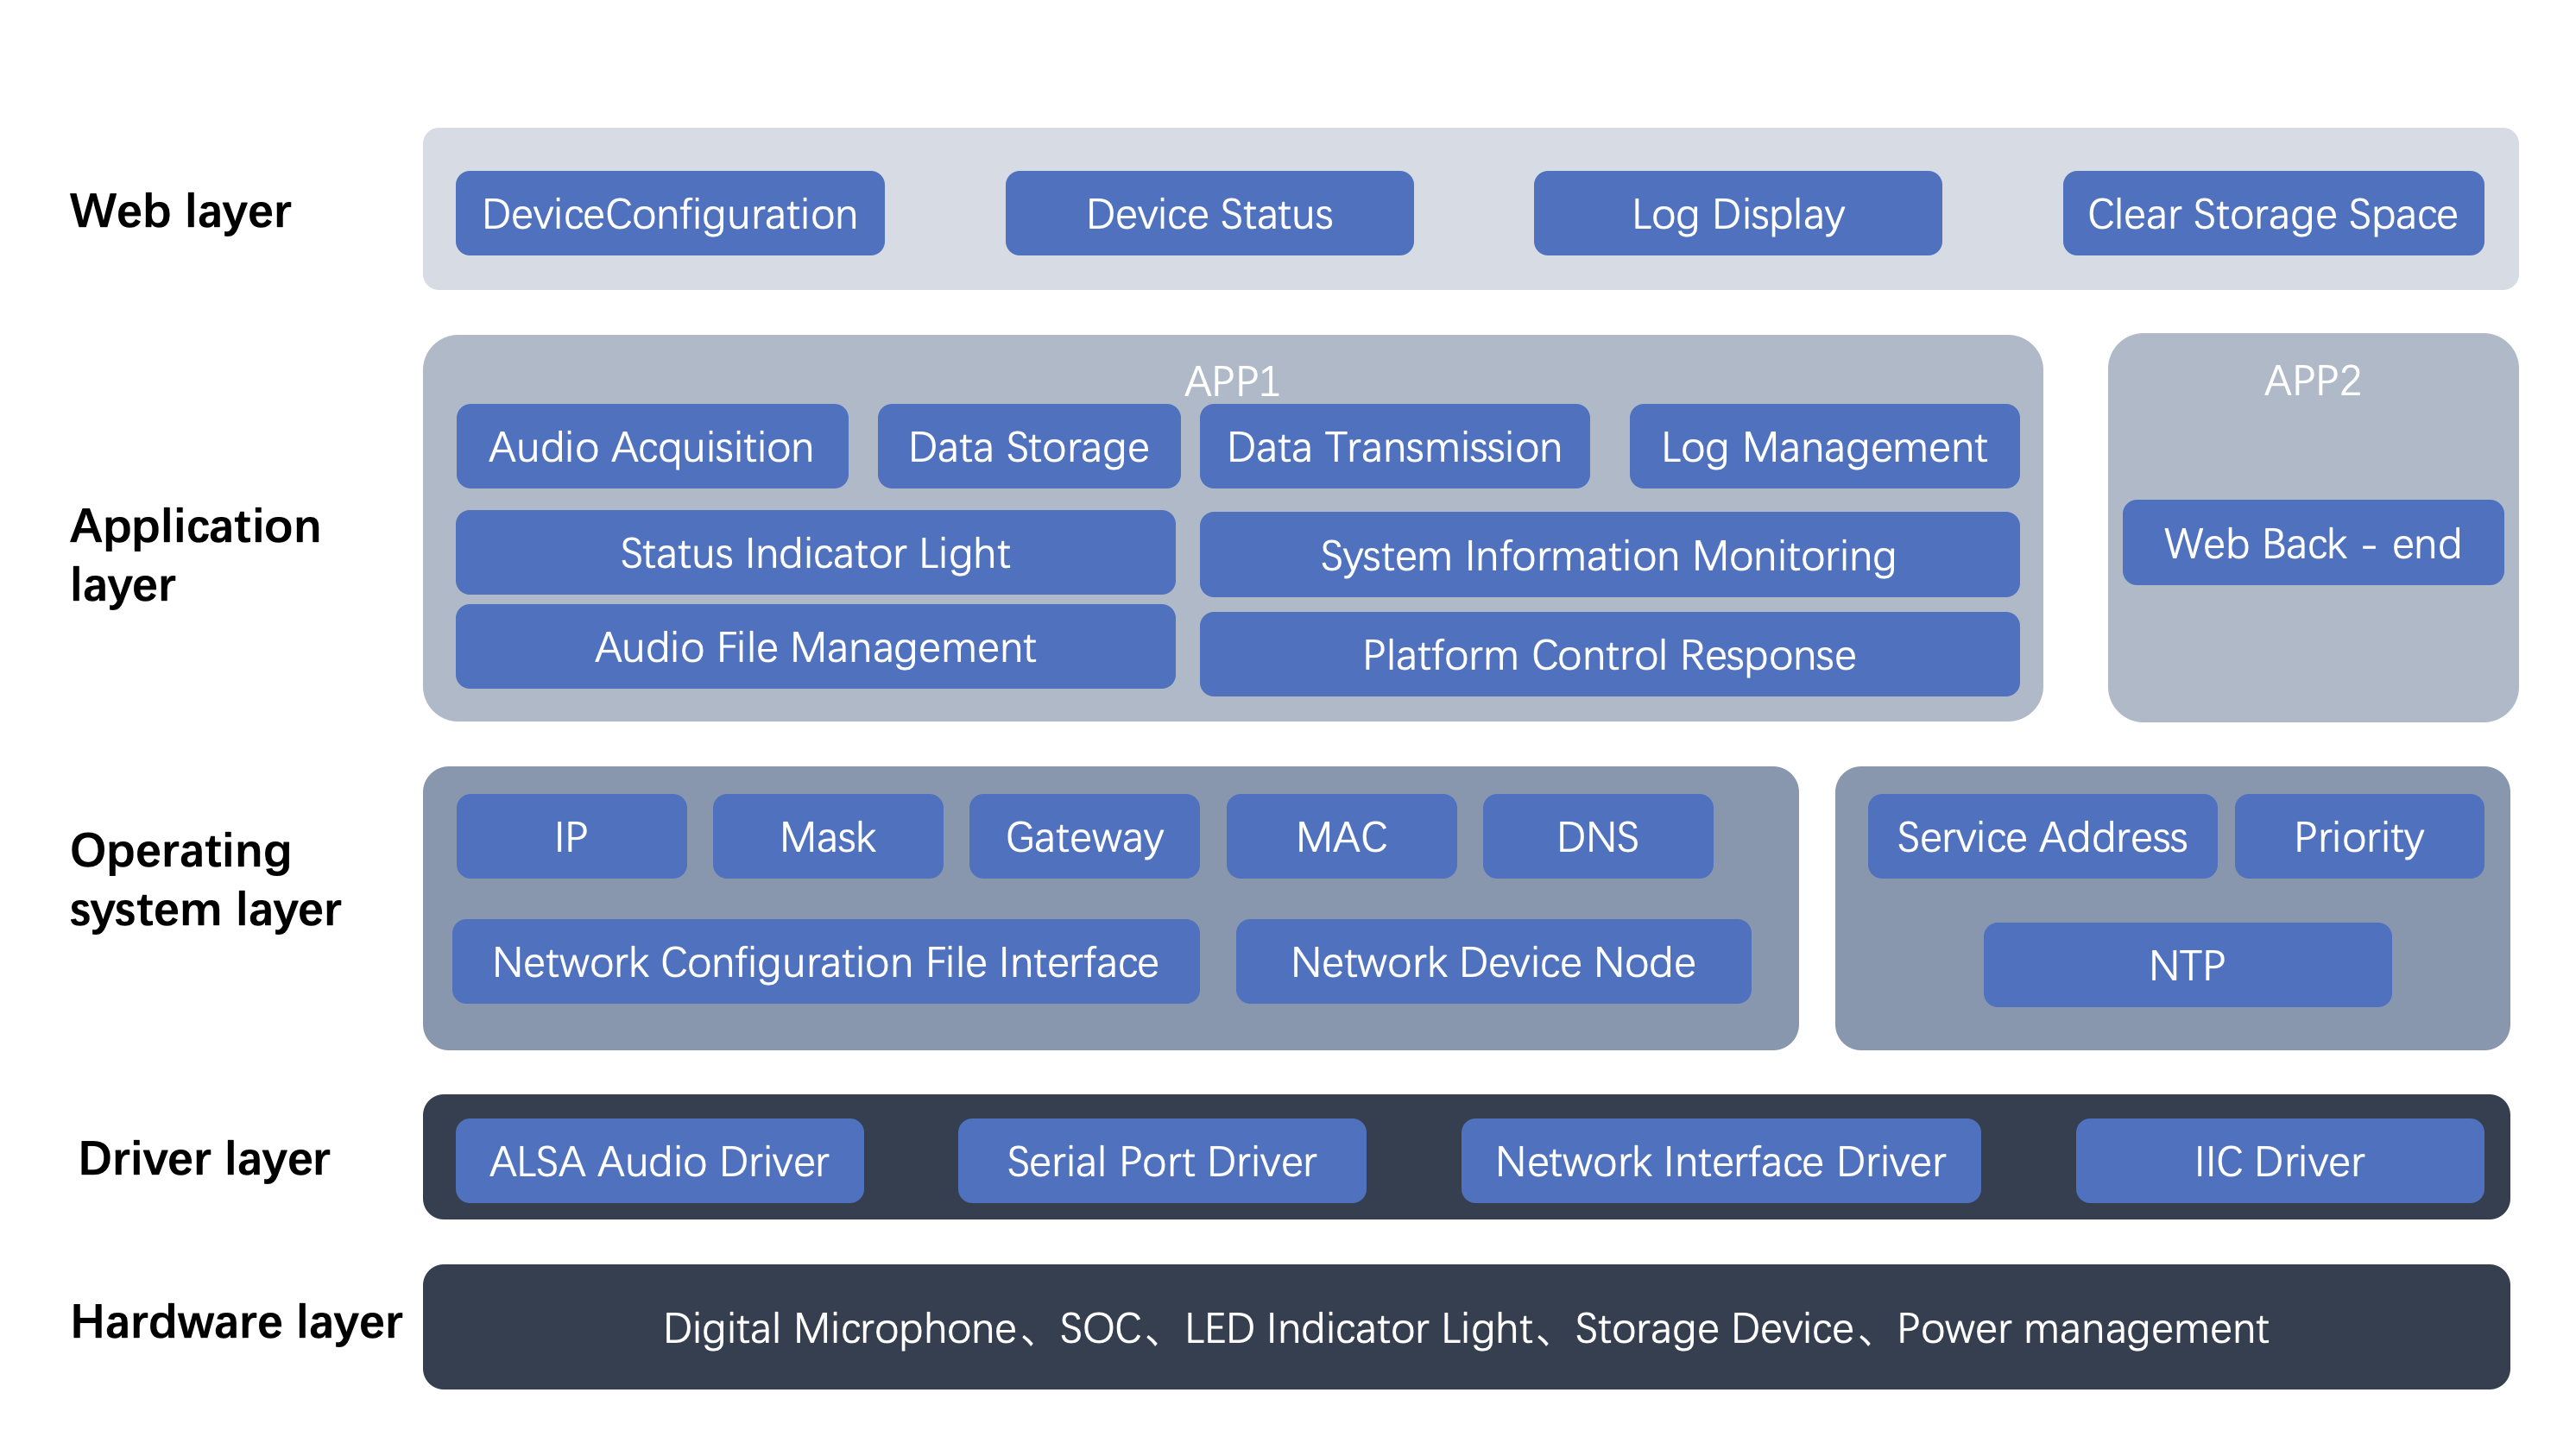
\includegraphics[width=0.8\textwidth]{./系统框架图.png}
    \caption{System Architecture Diagram}
    \label{fig:system-architecture}
\end{figure}
\subsection{Working Flow}
Working flow is shown in the following figure.
\begin{figure}[htbp]
    \centering
    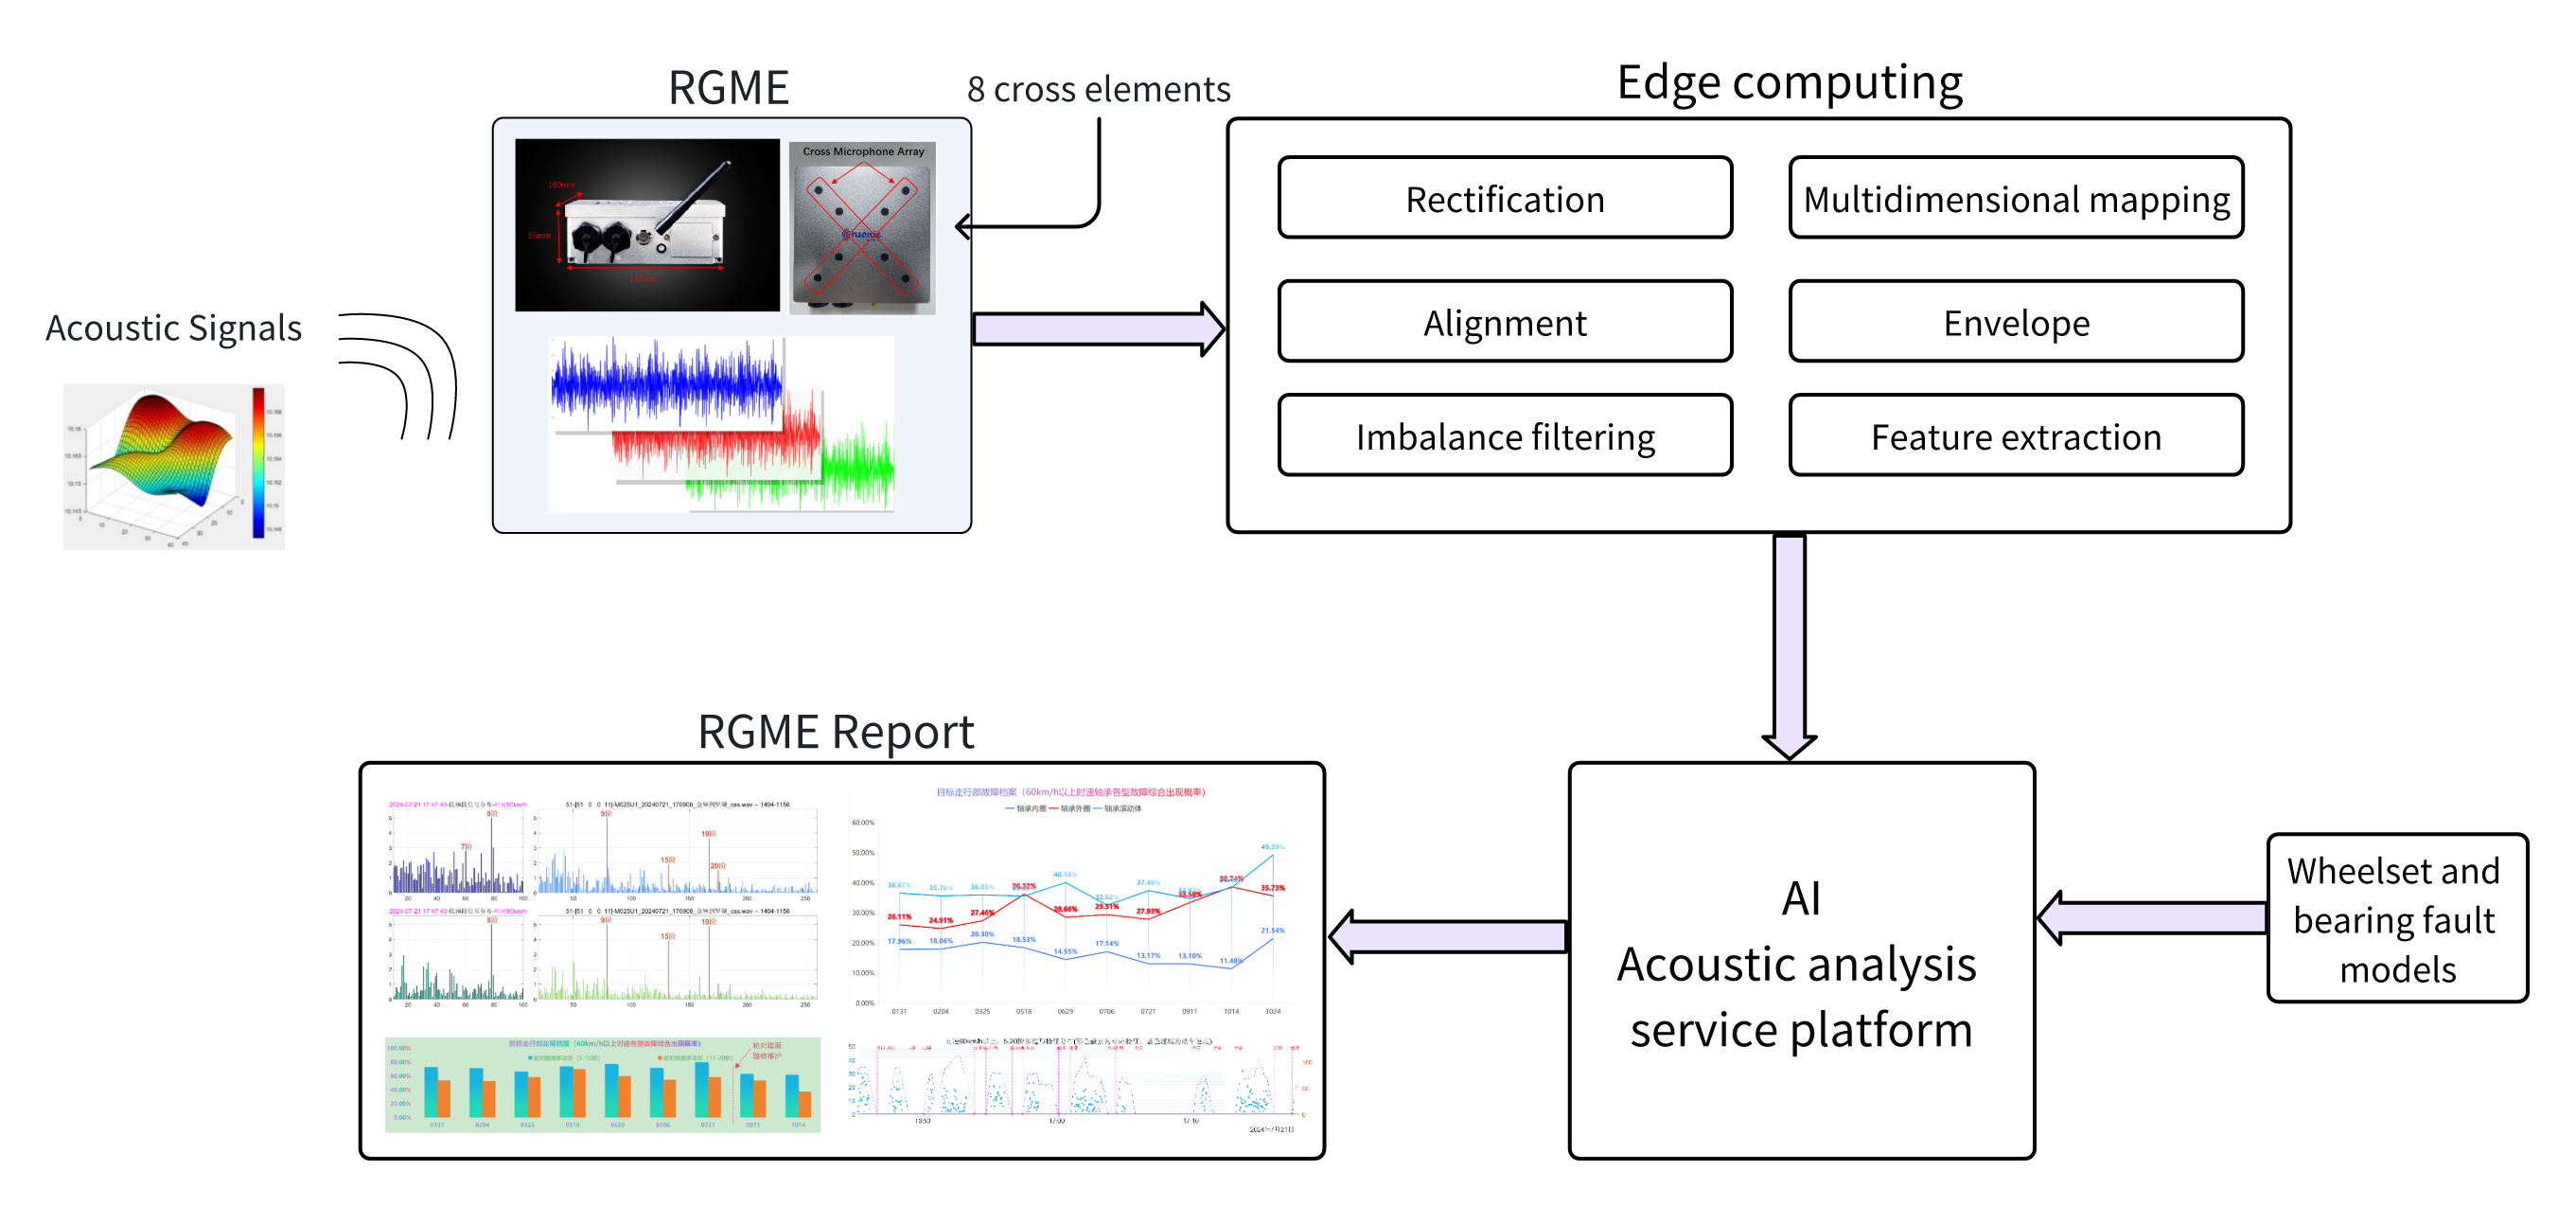
\includegraphics[width=0.8\textwidth]{./工作流程图.png}
    \caption{Working Flow Diagram}
    \label{fig:working-flow}
\end{figure}
When the RGME device is powered on, it will automatically start the system and enter the working state. The device will automatically detect the microphone status, and if the microphone is not connected, it will automatically enter the self-check state. If the microphone is connected, it will enter the working state. The RGME device will continuously collect acoustic signals from the microphones, and after several edge compute functions process, the raw data can be transfered into preprocessed signal data, it will store them in the storage module.

The preprocessed data can be downloaded via the local web interface or the X-code interface. After download the data, the data can be transfered to ENSONIC's server for further analysis and processing. The detailed transfer way should be discussed later.

Because the RGME device could not connect to the train signal network bus, MTR should provide wheelset diameters and train speed record to generate reports.

\subsection{Function Modules}
\begin{enumerate}
    \item Audio Signal Acquisition Module
    \begin{itemize}
        \item Acquire audio data using ALSA library functions
        \item Support for custom configuration of acquisition data channels
        \item Can be codec configured, including phase adjustment, digital gain, gain calibration, high/low pass filters, etc.
    \end{itemize}
    \item Data Storage Module
    \begin{itemize}
        \item Store the captured audio data as PCM and WAV format files
        \item Configurable storage location (SD card, USB stick), storage data channel, and duration of a single storage file
        \item Support file size and storage space threshold management, automatically delete old files
    \end{itemize}
    \item Data transmission Module
    \begin{itemize}
        \item Scaling PCM data into an agreed format (DSMQTT){\bfseries\emph{Not used in this project}}
        \item Upload data to the platform using the MQTT protocol {\bfseries\emph{Not used in this project}}
        \item Configurable MQTT protocol part parameters, data transmission network interface card, data packet size (interval), data channel {\bfseries\emph{Not used in this project}}
    \end{itemize}
    \item Log Management Module
    \begin{itemize}
        \item Record the system operation log, including audio acquisition, data storage, data transmission, platform control and other information
        \item Support log level setting, log file size limit, log file management and other functions
    \end{itemize}
    \item Status Indication Module
    \begin{itemize}
        \item Use LED indicators to display device status, including communication status, acquisition status, storage status, and working status
    \end{itemize}
    \item Platform Control Response Module
    \begin{itemize}
        \item Receive control instructions issued by the platform, such as device status light control, audio data issued by the platform {\bfseries\emph{Not used in this project}}
        \item Execute the corresponding operation and return the execution result {\bfseries\emph{Not used in this project}}
    \end{itemize}
    \item System Monitoring Module
    \begin{itemize}
        \item Get real-time information about the system runtime, such as CPU usage, memory usage, storage space usage, device IP, etc
        \item Log real-time information and upload it to the platform {\bfseries\emph{Not used in this project}}
    \end{itemize}
    \item Web Module
    \begin{itemize}
        \item Provides a web configuration page for easy device configuration and management
        \item Provide device status and log display to facilitate users to view device status
        \item Storage space management function to easily empty storage data
        \item The front end uses HTML + Layui, and the back end uses Python 3.6 web.py framework
    \end{itemize}
\end{enumerate}
\clearpage
\section{Working Principle}
\subsection{Rolling Bearing Fault Diagnosis Principle}
Rolling bearings are one of the key components of the running part of the train. Good operation of the bearings is the premise to ensure the safe operation of the train. In order to ensure the safe and reliable operation of the train, it is essential to regularly check and maintain the bearings.
The causes of rolling bearing failure are complex and diverse. Factors such as heavy loads, complex loads, excessive speed or acceleration, and extreme temperatures may all cause early failure. In addition, improper mechanical assembly and neglect of operating norms will also exacerbate this problem. The following is a brief analysis of the main types of failure of rolling bearings and their causes:
\begin{enumerate}
    \item Wear: mainly caused by foreign body intrusion and insufficient lubrication. Wear usually occurs on the contact surface of the bearing inner ring, outer ring and rolling element, resulting in increased bearing clearance, decreased working accuracy and shortened service life, accompanied by increased vibration and noise.
    \begin{figure}[htbp]
        \centering
        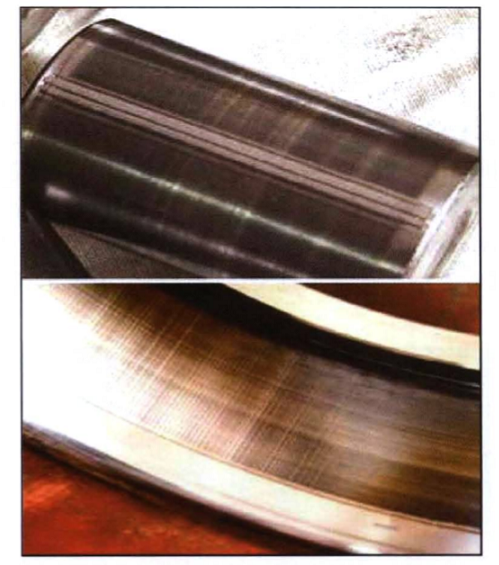
\includegraphics[width=0.8\textwidth]{./滚体擦伤.png}
        \caption{Bearing Scratch}
        \label{fig:bear-scratch}
    \end{figure}
    \item Fatigue spalling: Rolling bearings are subjected to alternating loads for a long time, and cracks will occur between the rolling elements and the inner and outer rings, usually in the area of maximum shear force. As the bearing runs for more time, the cracks gradually expand, eventually leading to contact surface spalling, which in turn increases the impact load and the degree of failure.
    \item Corrosion: The corrosion of rolling bearings mainly includes three types: chemical corrosion, electrical corrosion and micro-vibration corrosion. Chemical corrosion is caused by corrosive liquids, and electrical corrosion is caused by electric sparks generated by electric currents. The micro-vibration corrosion mainly occurs on the ferrule and is caused by small relative movements.
    \item Plastic deformation: Dents or scratches on the surface of the rolling element and raceway due to overload, impact, improper installation or intrusion of hard objects. These defects can increase the impact load between the rolling element and the inner and outer rings, thereby aggravating the failure and causing plastic deformation of the bearing.
    \item Fracture: When subjected to overload, the components of the rolling bearing may break, which in turn affects its normal operation. In addition, if there is a problem in the grinding, heat treatment or assembly process, the residual stress inside the component will increase, which will cause fracture.
    \item Glue: When two metal surfaces adhere to each other, it is called gluing. The main reason is that the excess heat generated by the rolling bearing cannot be dissipated in time, which is usually related to insufficient lubrication, high-speed movement or excessive load. Glue failures mostly occur between the cage and the rolling elements.
    \item Cage damage: Improper assembly or overload can increase the friction between the cage and the rolling elements, causing the cage to deform, further causing friction to heat up, causing more failures, and even causing the rolling elements to get stuck, while increasing vibration and noise.
\end{enumerate}

In the process of train running, the complex track environment, wheel-rail contact and other external excitation factors interact with the internal structural characteristics of the bearing, machining and assembly errors and potential failures, causing the vibration of the bearing.

During train operation, bearings are affected by uneven external forces. This imbalance of external forces, as well as changes in the number of rolling elements, can lead to periodic fluctuations in bearing carrying capacity, which can lead to vibration and noise. In addition, manufacturing errors or inconsistencies in the dimensions of bearing rolling elements can also lead to changes in support stiffness, which can be a potential factor in vibration generation. Irregularities in bearing surfaces, such as corrugations or bumps, can also cause random vibration.

During assembly, if the degree of fastening is not strictly controlled, too loose may cause the bearing to move in the axial direction, and too tight may cause local component deformation or changes in clearance, which can lead to periodic vibration. In addition, improper lubrication conditions can significantly affect the friction characteristics of bearings, which can lead to vibration and noise. During the operation of the bearing, any shock load may excite its natural vibration frequency, especially the natural frequency of the outer ring is relatively low, so it is most susceptible to excitation. When analyzing the frequency spectrum of vibration or acoustic signals, the natural frequency of the outer ring is usually particularly significant. 

When there is a local defect in the bearing part, the collision between the rolling element and the inner and outer rings will produce an impact signal. This impact signal is significantly different from the vibration characteristics under normal working conditions, and the duration is extremely short. The impact frequency of each part is also different. This frequency is called the interval frequency of the local defect, which can reflect most of the fault conditions, so it is called the failure frequency of the bearing. In order to solve the problem of the failure frequency of the bearing, the following derivation can be made.
\begin{figure}
    \centering
    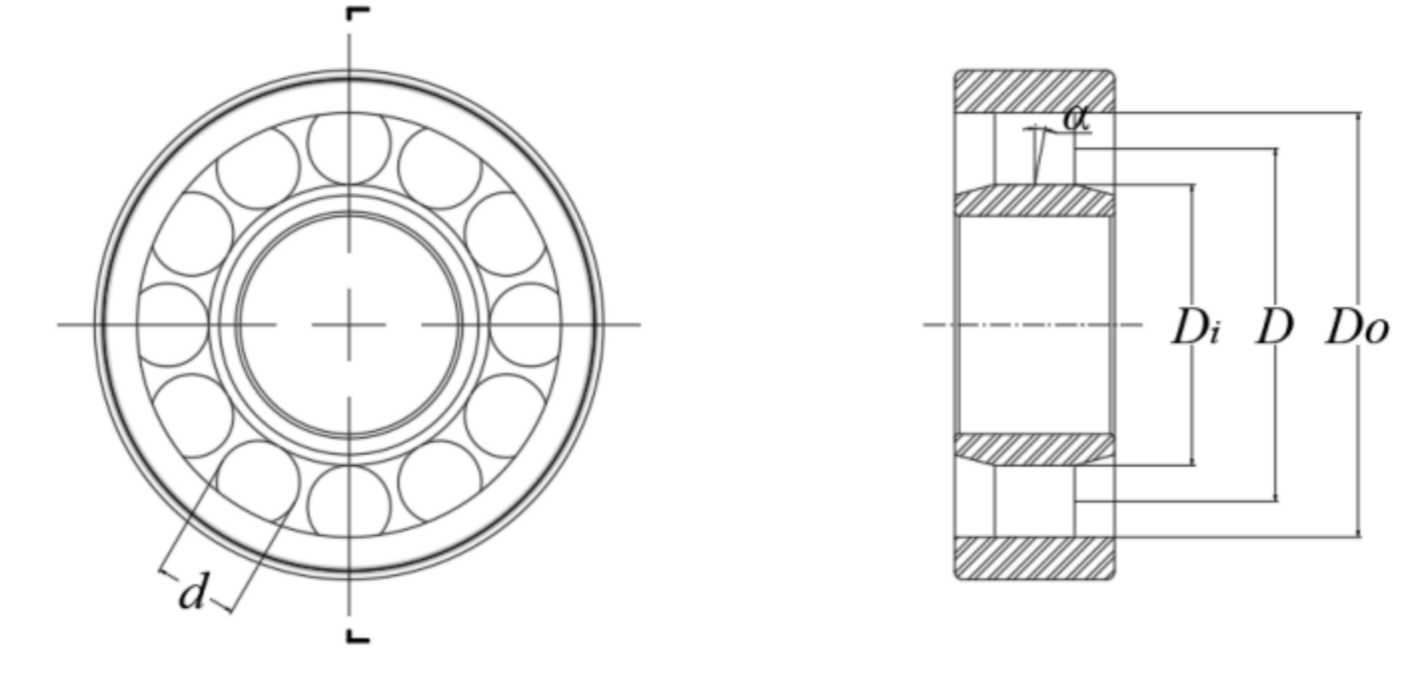
\includegraphics[width=0.8\textwidth]{./轴承结构简图.png}
    \caption{Bearing Structure Diagram}
    \label{fig:Bearing-structure}
\end{figure}

As shown in Figure \ref{fig:Bearing-structure}, let the diameter of the bearing rolling element be d, the diameter of the bearing inner ring is $D_i$ , the diameter of the bearing outer ring is $D_o$, the corresponding bearing middle diameter is D, the angular velocity of the outer ring is $\omega _o$, the angular velocity of the inner ring is $\omega_i$, and the contact angle between the rolling element and the inner ring raceway is $\alpha $. According to the geometric relationship, the relationship between the diameter of the inner and outer rings of the bearing and the diameter of the rolling element can be deduced, as shown in the following formula:

\begin{equation}
    D_i = D - d \cos\alpha
    \label{eq:2.1}
\end{equation}

\begin{equation}
    D_o = D + d \cos\alpha
    \label{eq:2.2}
\end{equation}


\begin{equation}
    v_i = \frac{1}{2} \cdot w_i \cdot D_i
    \label{eq:2.3}
\end{equation}

\begin{equation}
    v_o = \frac{1}{2} \cdot w_o \cdot D_o
    \label{eq:2.4}
\end{equation}

The linear speed of inside and outside scrolling is shown in the formula \ref{eq:2.3} and \ref{eq:2.4}.

Assuming that the rolling element rolls purely in the raceway, and the rotational speed of the cage is the average of the rotational speed of the inner ring and the outer ring, the rotational linear speed of the cage is as shown in the formula \ref{eq:2.5}.

\begin{equation}
    v_c = \frac{1}{4} [\omega_b (D - d \cos a) + \omega_\omega (D + d \cos a)]
    \label{eq:2.5}
\end{equation}

According to the formula \ref{eq:2.5}, the angular velocity of the cage can be obtained as shown in the formula \ref{eq:2.6}.

\begin{equation}
    w_c = \frac{1}{2} \left[ \omega_b \left( 1 - \frac{d}{D} \cos a \right) + \omega_\omega \left( 1 + \frac{d}{D} \cos a \right) \right]
    \label{eq:2.6}
\end{equation}

Since $\omega = 2 \pi f$, the rotation frequency of the cage is as shown in the formula \ref{eq:2.6}.

\begin{equation}
    f_c = \frac{1}{2} \left[ f_i \left( 1 - \frac{d}{D} \cos a \right) + f_o \left( 1 + \frac{d}{D} \cos a \right) \right]
    \label{eq:2.7}
\end{equation}

If the outer ring is fixed, then $f_o = 0$, so the formula \ref{eq:2.7} can be reduced to the formula \ref{eq:2.8}.

\begin{equation}
    f_c = \frac{1}{2} f_i \left( 1 - \frac{d}{D} \cos a \right)
    \label{eq:2.8}
\end{equation}

Formula \ref{eq:2.8} is also the rotation frequency of the cage relative to the outer ring. The rotation frequency of the cage relative to the inner ring is shown in Formula \ref{eq:2.9}.

\begin{equation}
    f_\alpha = f_i - f_c = \frac{1}{2} f_i \left( 1 + \frac{d}{D} \cos a \right)
    \label{eq:2.9}
\end{equation}

The rotation frequency of the roller is shown in the formula \ref{eq:2.10}.

\begin{equation}
    f_{bt} = f_{ci} \frac{D_i}{d} = \frac{1}{2} f_i \frac{D}{d} \left[ 1 - \left( \frac{d}{D} \cos a \right)^2 \right]
    \label{eq:2.10}
\end{equation}

The rotation of the cage relative to the inner ring causes the rolling elements to pass n times at the same contact point of the inner ring, where n represents the total number of rolling elements. The failure frequency of the bearing can be deduced by multiplying the relative rotation frequency of the component by the number of times it has passed. In the case of the inner ring rotating and the outer ring stationary, the rotation frequency of the bearing is the same as the rotation frequency of the inner ring. According to formula \ref{eq:2.11}, the failure frequency of the outer ring of the rolling bearing can be calculated:

\begin{equation}
    f_o = \frac{1}{2} \cdot \frac{r}{60} \cdot n \cdot \left( 1 - \frac{d}{D} \cos a \right)
    \label{eq:2.11}
\end{equation}

The calculation of the failure frequency of the inner ring of the rolling bearing is shown in the formula \ref{eq:2.12}.

\begin{equation}
    f_i = \frac{1}{2} \cdot \frac{r}{60} \cdot n \cdot \left( 1 + \frac{d}{D} \cos a \right)
    \label{eq:2.12}
\end{equation}

The calculation of the failure frequency of rolling bearings and rolling elements is shown in the formula \ref{eq:2.13}.

\begin{equation}
    f_b = \frac{1}{2} \cdot \frac{r}{60} \cdot \frac{D}{d} \cdot \left( 1 - \left( \frac{d}{D} \right)^2 \cdot \cos^2 a \right)
    \label{eq:2.13}    
\end{equation}

The failure frequency calculation of the friction between the rolling bearing cage and the outer ring is shown in the formula \ref{eq:2.14}.

\begin{equation}
    f_{co} = \frac{1}{2} \cdot \frac{r}{60} \cdot \left( 1 - \frac{d}{D} \cos a \right)
    \label{eq:2.14}
\end{equation}

The failure frequency calculation of the friction between the rolling bearing cage and the inner ring is shown in the formula \ref{eq:2.15}.
\begin{equation}
    f_{ci} = \frac{1}{2} \cdot \frac{r}{60} \cdot \left( 1 + \frac{d}{D} \cos a \right)
    \label{eq:2.15}
\end{equation}

In the formulas \ref{eq:2.11} to \ref{eq:2.15}:
\begin{itemize}
    \item $f_o$ is the failure frequency of the outer ring of the rolling bearing (Hz);
    \item $f_i$ is the failure frequency of the inner ring of the rolling bearing (Hz);
    \item $f_b$ is the failure frequency of the rolling element of the rolling bearing (Hz);
    \item $f_{co}$ and $f_{ci}$ is the failure frequency of the friction between the rolling bearing cage and the outer ring (Hz);
    \item $r$ is the rotational speed of the rolling bearing (r/min);
    \item $n$ is the number of rolling elements of the bearing;
    \item $d$ is the diameter of the rolling element of the bearing (mm);
    \item $D$ is the diameter of the rolling bearing pitch circle (mm);
    \item $\alpha$ is the contact angle of the rolling element.
\end{itemize}

In order to solve the interference of non-stationary signal frequency conversion on fault frequency under variable speed conditions, ENSONIC research team use the fault characteristic order ratio to characterize the fault frequency characteristics. Compared with the traditional fault frequency calculation formula, the calculation method of the fault characteristic order ratio is simpler, and there is no need to introduce the independent variable of frequency conversion. For the specific calculation formula, please refer to the table \ref{tab:order-ratio}.

\begin{table}
    \centering
    \caption{Rolling Bearing Fault Characteristic Ratio Calculation Formula}
    \label{tab:order-ratio}
    \begin{tabular}{|c|c|}
        \hline
        \toprule
        Feature Order Ratio & Formula \\
        \midrule
        Outer ring fault characteristic order ratio $O_o$ & $\frac{n}{2} \cdot \left( 1 - \frac{d}{D} \cos \alpha \right)$ \\ \hline
        Inner ring fault characteristic order ratio $O_i$ & $\frac{n}{2} \cdot \left( 1 + \frac{d}{D} \cos \alpha \right)$ \\   \hline
        Rolling element fault characteristic order ratio $O_b$ & $\frac{n}{2} \cdot \left( 1 - \left( \frac{d}{D} \right)^2 \cos^2 \alpha \right)$ \\   \hline
        Cage friction fault characteristic order ratio $O_{c}$ & $\frac{1}{2} \cdot \left( 1 \pm \frac{d}{D} \cos \alpha \right)$ \\ \hline
        \bottomrule
    \end{tabular}
\end{table}

\subsection{Wheel Tread Fault Diagnosis Principle}

As an important driving part of a vehicle, the health of wheels is directly related to the safety and efficiency of operation. Due to the operational characteristics such as fast start, frequent braking and start-stop, and poor track line status, the wheel tread of trains is at risk of various failures. The common forms of train wheel tread damage are local wheel damage such as flat scar and peeling, and full-circumferential wheel damage such as pit wear and wheel polygon. In addition to this, it also includes defects such as trauma, delamination, collapse, etc. The impact of these damages on the dynamic response of wheels and rails is similar to that of local wheel damage.

Tread failure not only exacerbates the wear and tear of the moving parts of the vehicle, but also induces vibration and noise problems, which affect the comfort of passengers. In some cases, wheel tread failure may also cause excessive local loads, resulting in unstable operation and increased safety risks. In addition, uneven tread wear can also affect the dynamic characteristics of the wheelset, increasing the dynamic wheel weight and accelerating the wear of the track structure.

Wheel thread out of roundness involves a variety of factors, such as the irregular initial shape of the wheel and the vibration excitation of the wheel and rail during long-term operation. The out of roundness can be divided into two types: partial out of roundness and full-circumference out of roundness. The partial out of roundness refers to the appearance of some radial defects on the wheel tread, such as scratches or peeling. The full-circumference out of roundness is mainly manifested as the wheel polygon, that is, the wheel radius changes periodically on the entire circumference.

When the train is running, the contact between the normal wheel tread and the rail will generate low-frequency and relatively stable noise; conversely, when the irregular wheel passes through the rail, it will cause abnormal impact vibration noise with different periodicity. Therefore, by analyzing the characteristics of the noise acoustic signal, potential causes of wheel roundness can be identified.

Scratches and peeling are common tread failures.Figure \ref{fig:wheel-rolling} is a schematic diagram of the faulty wheel running.
\begin{figure}[htbp]
    \centering
    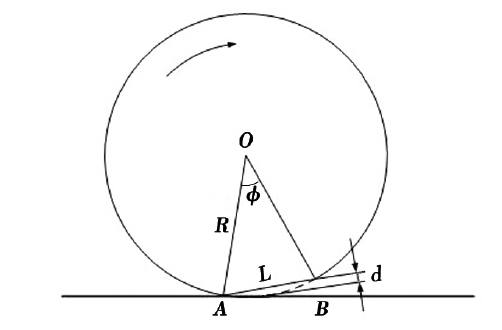
\includegraphics[width=0.8\textwidth]{./Wheel rolling.png}
    \caption{Wheel Rolling Schematic Diagram} 
    \label{fig:wheel-rolling}
\end{figure}

At low speed, when the wheel rolls to the starting point A of the abrasion, it rotates with point A as the center of the circle and the length L of the abrasion as the radius until the entire abrasion surface touches the track. When all the abrasion surfaces hit the rail, the wheel will continue to rotate at the center of the abrasion termination point B, thus applying additional power to the track until the wheel returns to normal rotation.

At high speed, the wheel will detach from the rail surface after reaching point A, rotate in the air and move forward inertia, and finally contact the track at point B, resulting in a certain amplitude of impact. When the time required for the wheel to move from state A to state B is equal to the time required for the wheel center to fall, the speed reaches the critical state of wheel-rail impact.

During driving, if only a single fault exists, the impact frequency of the track will be equal to the rotation frequency of the wheel, $f = V_c / 2 \pi R$ ( $f$ is the impact frequency, $V_c$ is the running speed, $R$ is the wheel radius). When the running speed is $V_c$ less than the critical speed, the impact time $t_r$ between the tread and the rail, the vertical impact speed is $v_0$.

\begin{equation}
    t_r = \frac{L}{v_c} \approx \frac{2 \sqrt{2 R d}}{v_c}
    \label{eq:2.21}
\end{equation}

\begin{equation}
    v_0 = v_c \sin \frac{\phi}{2} \approx v_c \frac{1}{2} \frac{L}{R} \approx v_c \frac{\sqrt{2 R d}}{R}
    \label{eq:2.22}
\end{equation}

The impact mechanical kinetic energy generated during the impact process is.

\begin{equation}
    E_M = \frac{1}{2} M v_0^2 = M v_c^2 \frac{d}{R}
    \label{eq:2.23}
\end{equation}

Where $M$ is the mass of the wheel, $d$ is the depth of the abrasion.

When the running speed $V_c$ is greater than the critical speed, the impact time $t_r$ and vertical impact speed $v_0$ between the tread and the rail are:

\begin{equation}
    t_r = \frac{L}{v_c + \sqrt{\mu R}} \approx \frac{2 \sqrt{2 R d}}{v_c + \sqrt{\mu R}}
    \label{eq:2.24}
\end{equation}

\begin{equation}
    v_0 = \frac{\mu L}{v_c + \sqrt{\mu R}} \approx \frac{2 \mu \sqrt{2 R d}}{v_c + \sqrt{\mu R}}
    \label{eq:2.25}    
\end{equation}

\begin{equation}
    \mu = \frac{M_1 + M_2}{M_2} g
    \label{eq:2.26}    
\end{equation}

Where $M_1$ is the sprung mass, $M_2$ is the unsprung mass, and $g$ is the acceleration of gravity.

The impact mechanical kinetic energy generated during the impact process is:
\begin{equation}
    E_M = \frac{1}{2} M v_0^2 = 4 M \frac{\mu^2 R d}{(v_c + \sqrt{\mu R})^2}
    \label{eq:2.27}    
\end{equation}

According to the above analysis, tread failure will cause periodic vibration and shock between the wheel and the track. As the running speed increases, the impact effect between the wheel and the track will also increase. At the critical speed, the impact effect reaches its maximum value, after which it will gradually weaken and eventually stabilize.

The wheel polygon is a manifestation of the irregular shape of the wheel, which can be mathematically modeled by summing the harmonic waves of different orders. Theory and practice show that the order of the wheel polygon is usually between 1 and 20. In most cases, the wheel polygon is dominated by one of the orders.

When the train is running, if there is a wheel polygon, there will be a periodic dynamic force between the wheels and rails, resulting in shock and vibration of the wheel-rail system, which will significantly affect the stability and durability of the vehicle and other components of the rail system.

The first-order wheel polygon, that is, the eccentricity of the wheel, is a typical harmonic excitation. Due to the action of centrifugal excitation, the wheel-rail system will produce periodic forced vibration, and the cycle of the wheel-rail force change is roughly equivalent to the time it takes for the wheel to complete a week.

The second-order wheel polygon shows the elliptical shape of the wheel, and the period of wheel-rail force change is about half of the time of wheel rolling. By analogy, the existence of wheel polygon will affect the vibration and radiation noise of the vehicle during operation, which will lead to the generation of periodic pulse and impact frequency. Impact frequency $f = n V_c / 2 \pi R$ ($n$ is the order of wheel polygon).
\clearpage
\section{Specifications of components}
\subsection{RGME Device}
The RGME device specifications are shown in the table \ref{tab:rgme-specs}.
\begin{table}[htbp]
    \centering
    \caption{RGME Device Specifications}
    \label{tab:rgme-specs}
    \begin{tabular}{|c|c|c|}
        \hline
        \toprule
        Class & Name & Specifications \\
        \midrule
        \multirow{6}{*}{Acoustic} & Microphone & 8\\ 
            \cline{2-3}
            & Frequency Response Range & 25Hz-22KHz(±3dB ref 1kHz)\\ 
            \cline{2-3}
            & Sensitivity & -37dBFs @1000Hz \\
            \cline{2-3} 
            & Dynamic Range & 28dBA to 120dBA \\
            \cline{2-3} 
            & Sampling Rate & $\leqslant$ 48KHz \\
            \cline{2-3} 
            & SNR & 66dBA @ 1kHz \\
            \cline{2-3} 
            & THD & 130.5dB @ 1kHz : 1\% THD \\
            \hline
        \multirow{6}{*}{Hardware} & OS & Linux embedded\\
            \cline{2-3}
            & CPU & ARM Cortex-A53\\
            \cline{2-3}
            & RAM & 1GB\\
            \cline{2-3}
            & eMMC & 8GB\\
            \cline{2-3}
            & Storage & up to 256GB\\
            \hline
        \multirow{2}{*}{Power} & Power Supply & DC12V\\
            \cline{2-3}
            & Power Consumption & $\leqslant$ 8W\\
            \hline
        \multirow{4}{*}{Interface} & Data & USB2.0 \& TF card\\
            \cline{2-3}
            & Ethernet & 10/100/1000Mbps POE supported\\
            \cline{2-3}
            & Power Interface & DC12V \& POE 48V\\
            \hline
        \multirow{5}{*}{Others} & Operating Temperature & -40°C to 70°C\\
            \cline{2-3}
            & Matrial & Aluminum alloy\\
            \cline{2-3}
            & Size & 160mm × 145mm × 55mm\\
            \cline{2-3}
            & Weight & 0.9kg\\
            \cline{2-3}
            & Protection Level & IP66\\
            \hline 
            \bottomrule
    \end{tabular}
\end{table}
\subsection{Power Module}
The power module specifications are shown in the table \ref{tab:power-specs}.
\begin{table}[htbp]
    \centering
    \caption{Power Module Specifications}
    \label{tab:power-specs}
    \begin{tabular}{|c|c|}
        \hline
        \toprule
        Name & Specifications \\
        \midrule
        Size & 140mm × 100mm × 50mm\\
        \hline
        Weight & 0.97kg\\
        \hline
        Power Input & AC 220V\\
        \hline
        Power Output & DC 12V\\
        \hline
        Total Reserve Power& $\approx$ 225W\\
        \hline
        \bottomrule
    \end{tabular}
\end{table}

\subsection{Battery Module}
The battery module specifications are shown in the table \ref{tab:battery-specs}.
\begin{table}[htbp]
    \centering
    \caption{Battery Module Specifications}
    \label{tab:battery-specs}
    \begin{tabular}{|c|c|}
        \hline
        \toprule
        Name & Specifications \\
        \midrule
        Size & 140mm × 100mm × 50mm\\
        \hline
        Weight & {\bfseries\emph{TBA}}\\
        \hline
        Power Output & DC 12V\\
        \hline
        Total Battery Capacity & 12V 9600mAh\\
        \hline
        \bottomrule
    \end{tabular}
\end{table}
\clearpage
\section{Electrical Schematic Diagrams}
\subsection{Power Module Schematic Diagram}
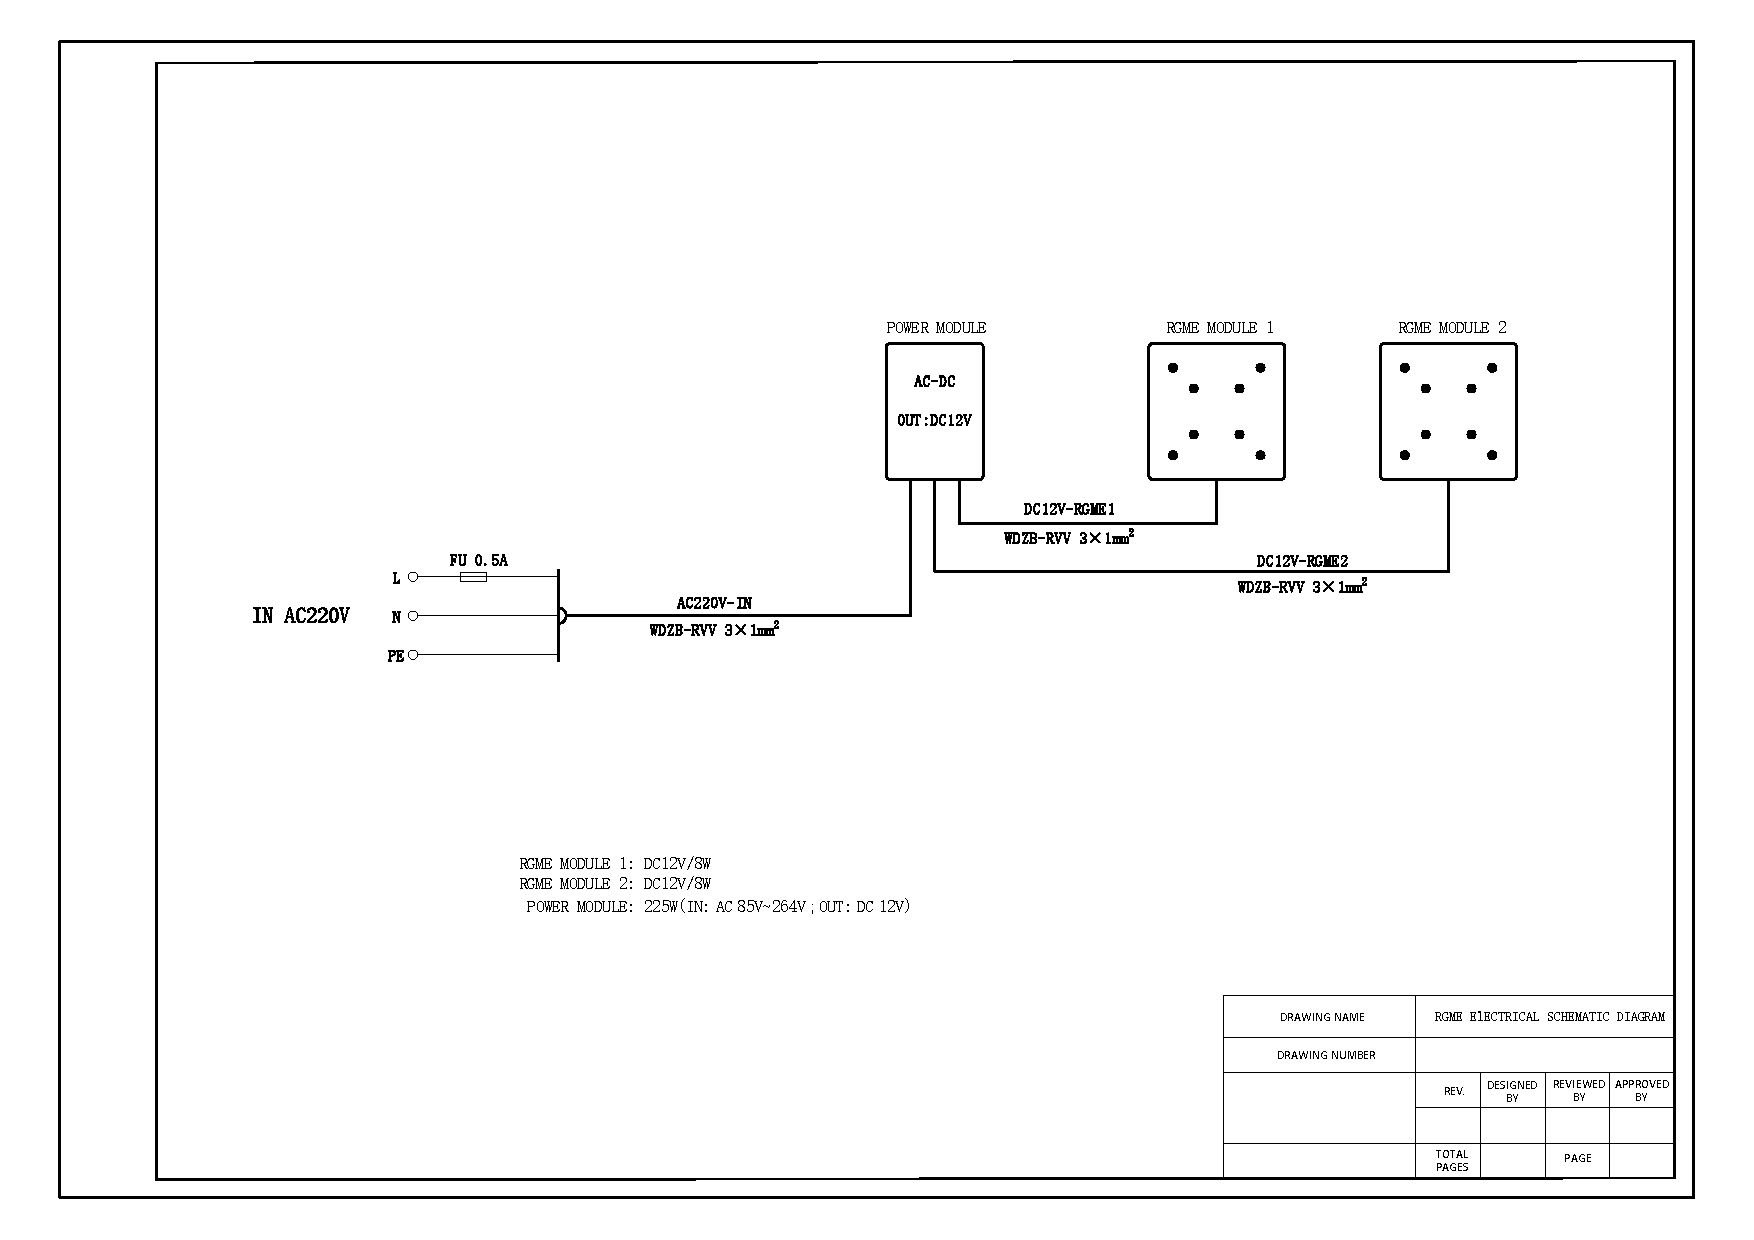
\includepdf[page={1-}, scale=0.75]{./走行部电源供电电气原理图.pdf}
\subsection{Battery Module Schematic Diagram}
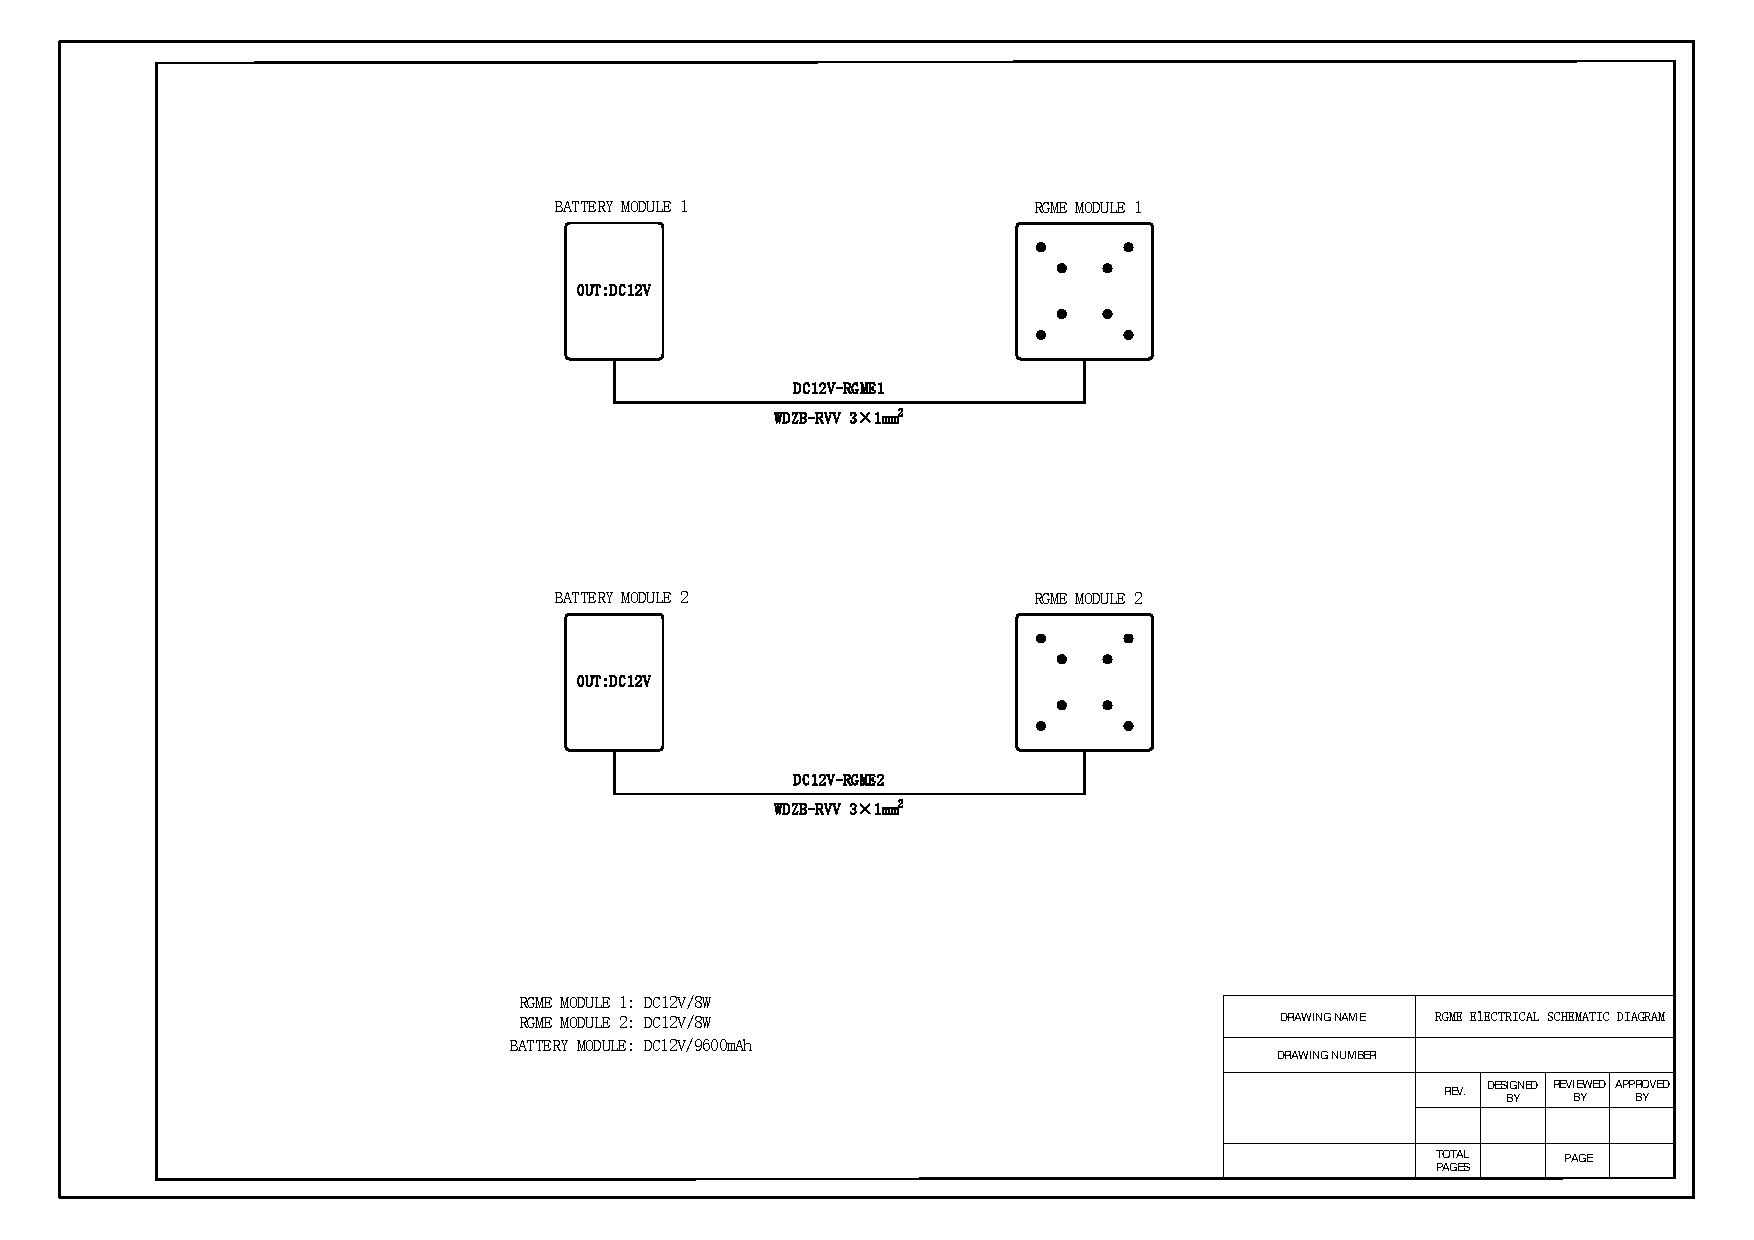
\includepdf[page={1-}, scale=0.75]{./走行部电气原理图_电池.pdf}
\clearpage
\section{Mechanical Design and Installation}
\subsection{Mechanical Design}
\subsubsection{RGME Device}
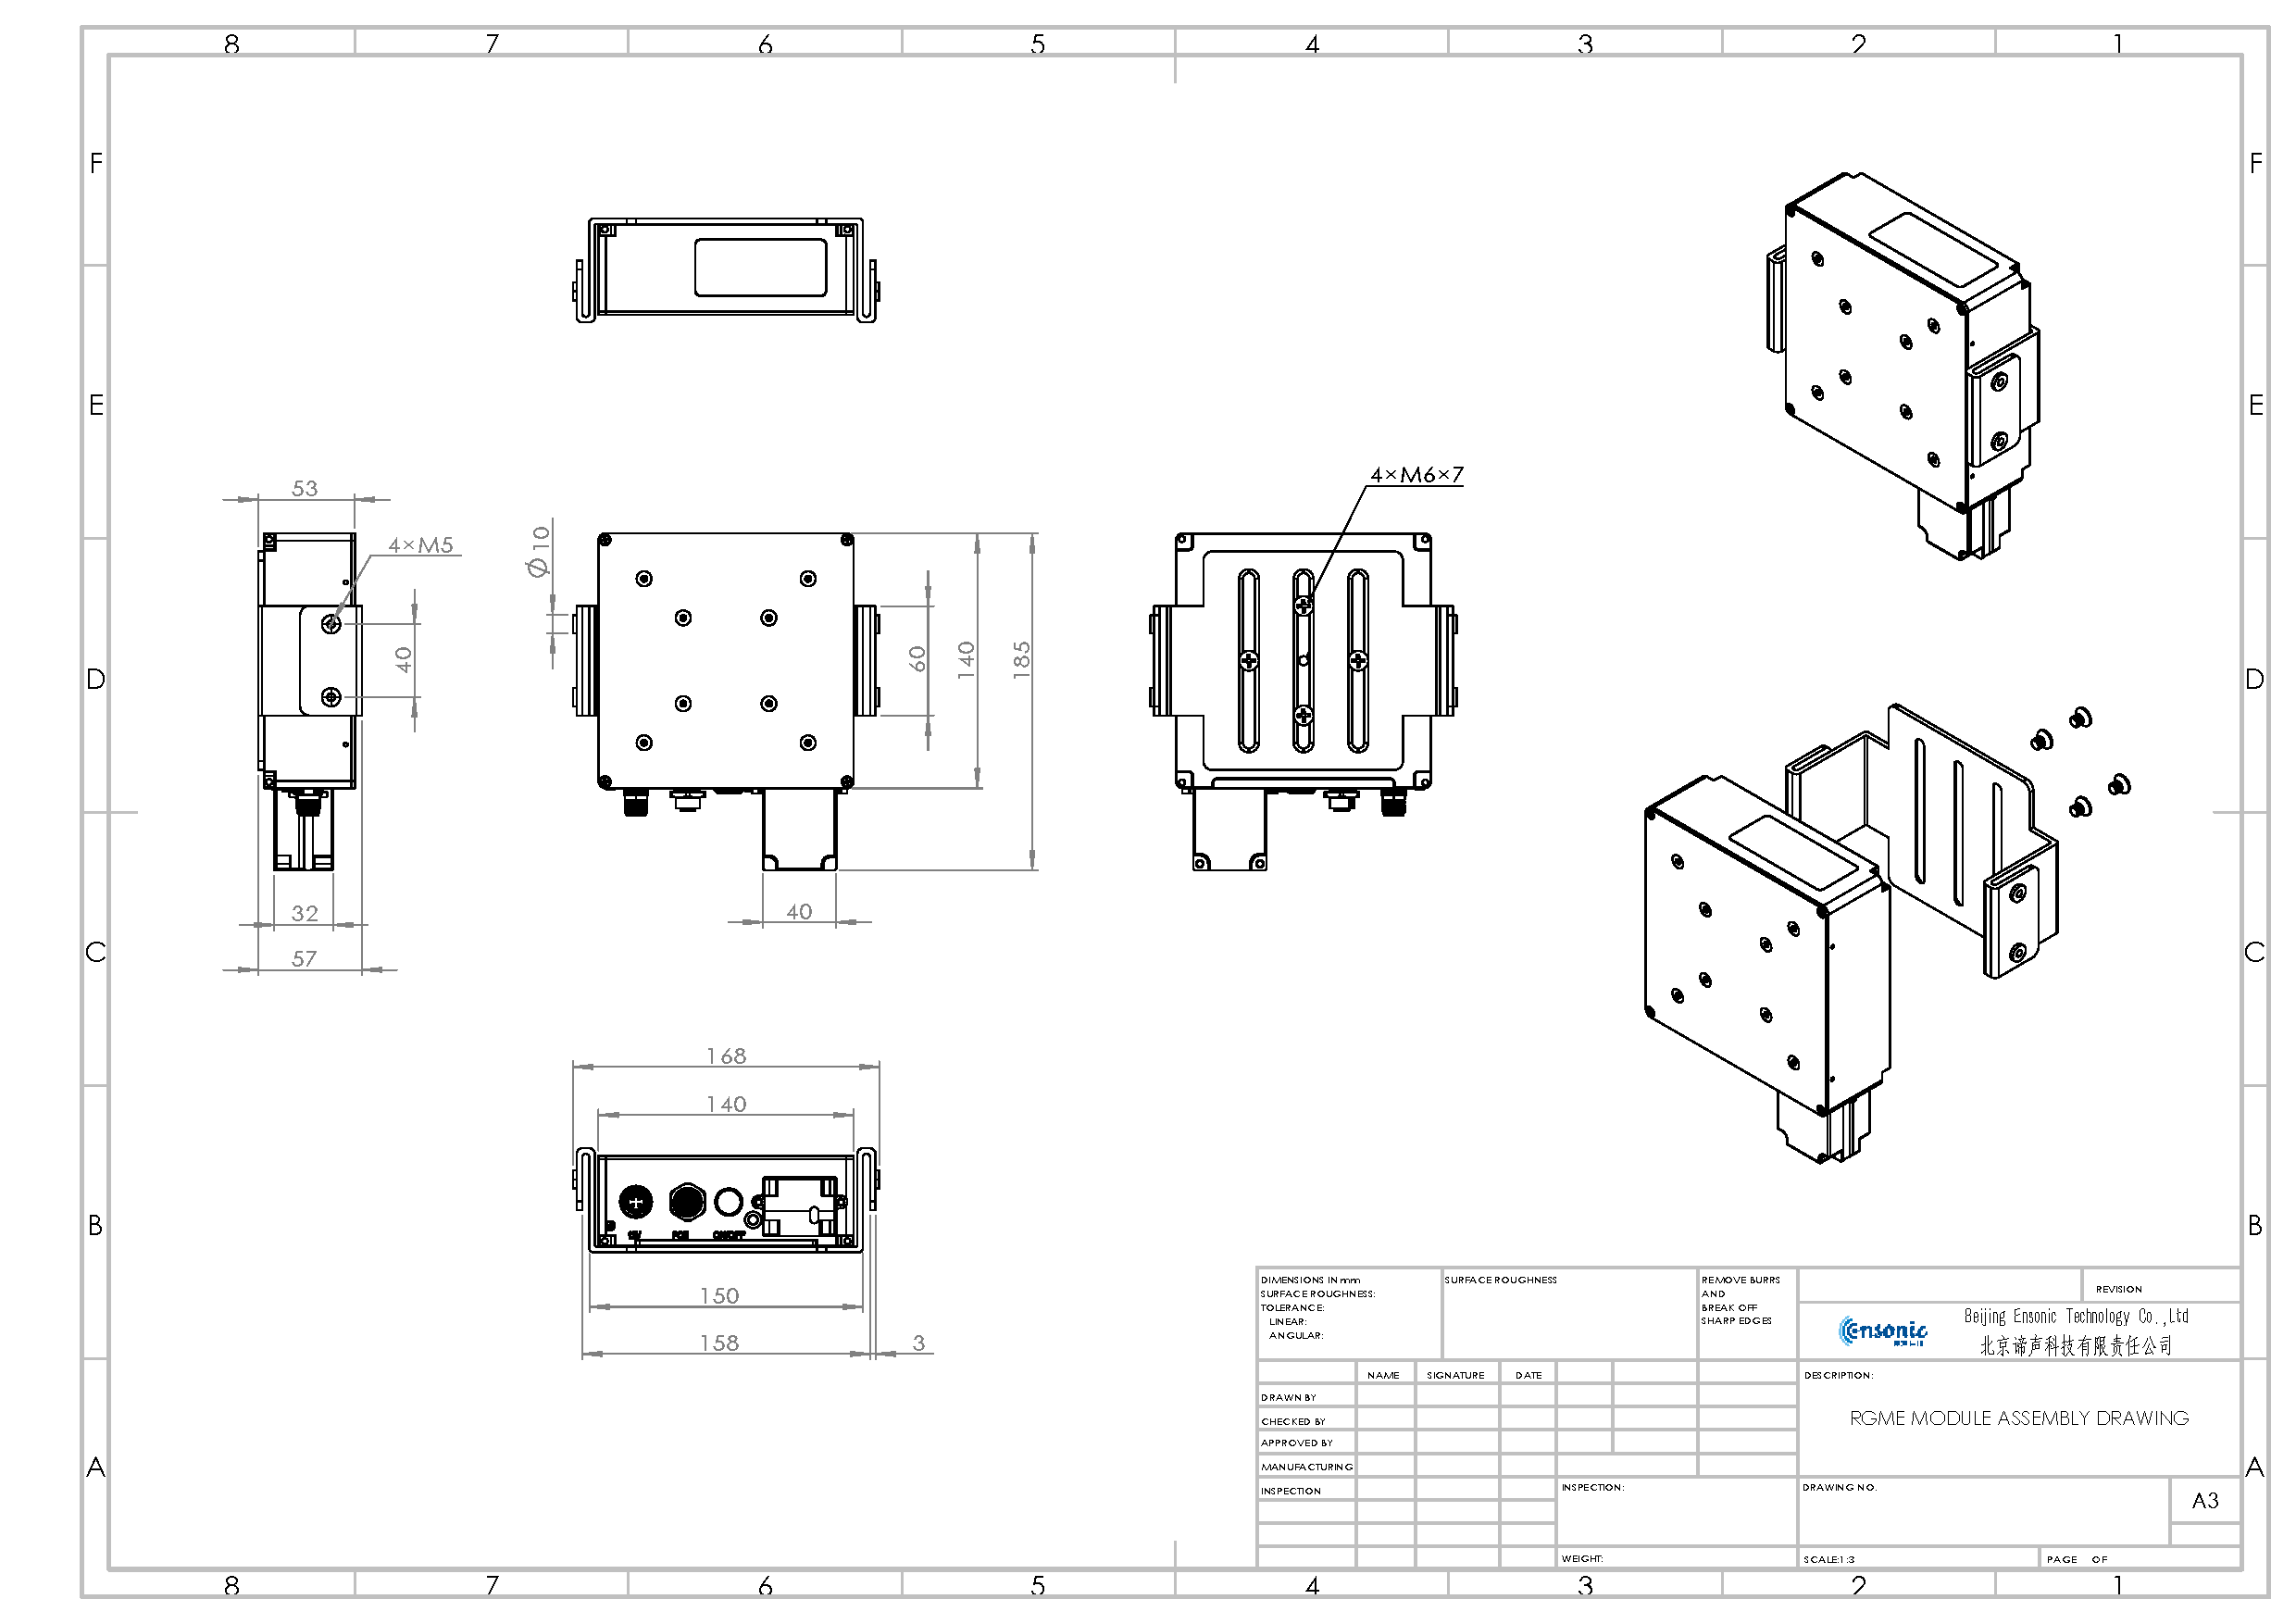
\includepdf[page={1-}, scale=0.75]{./声纹终端装配体.pdf}
\subsubsection{Battery Module}
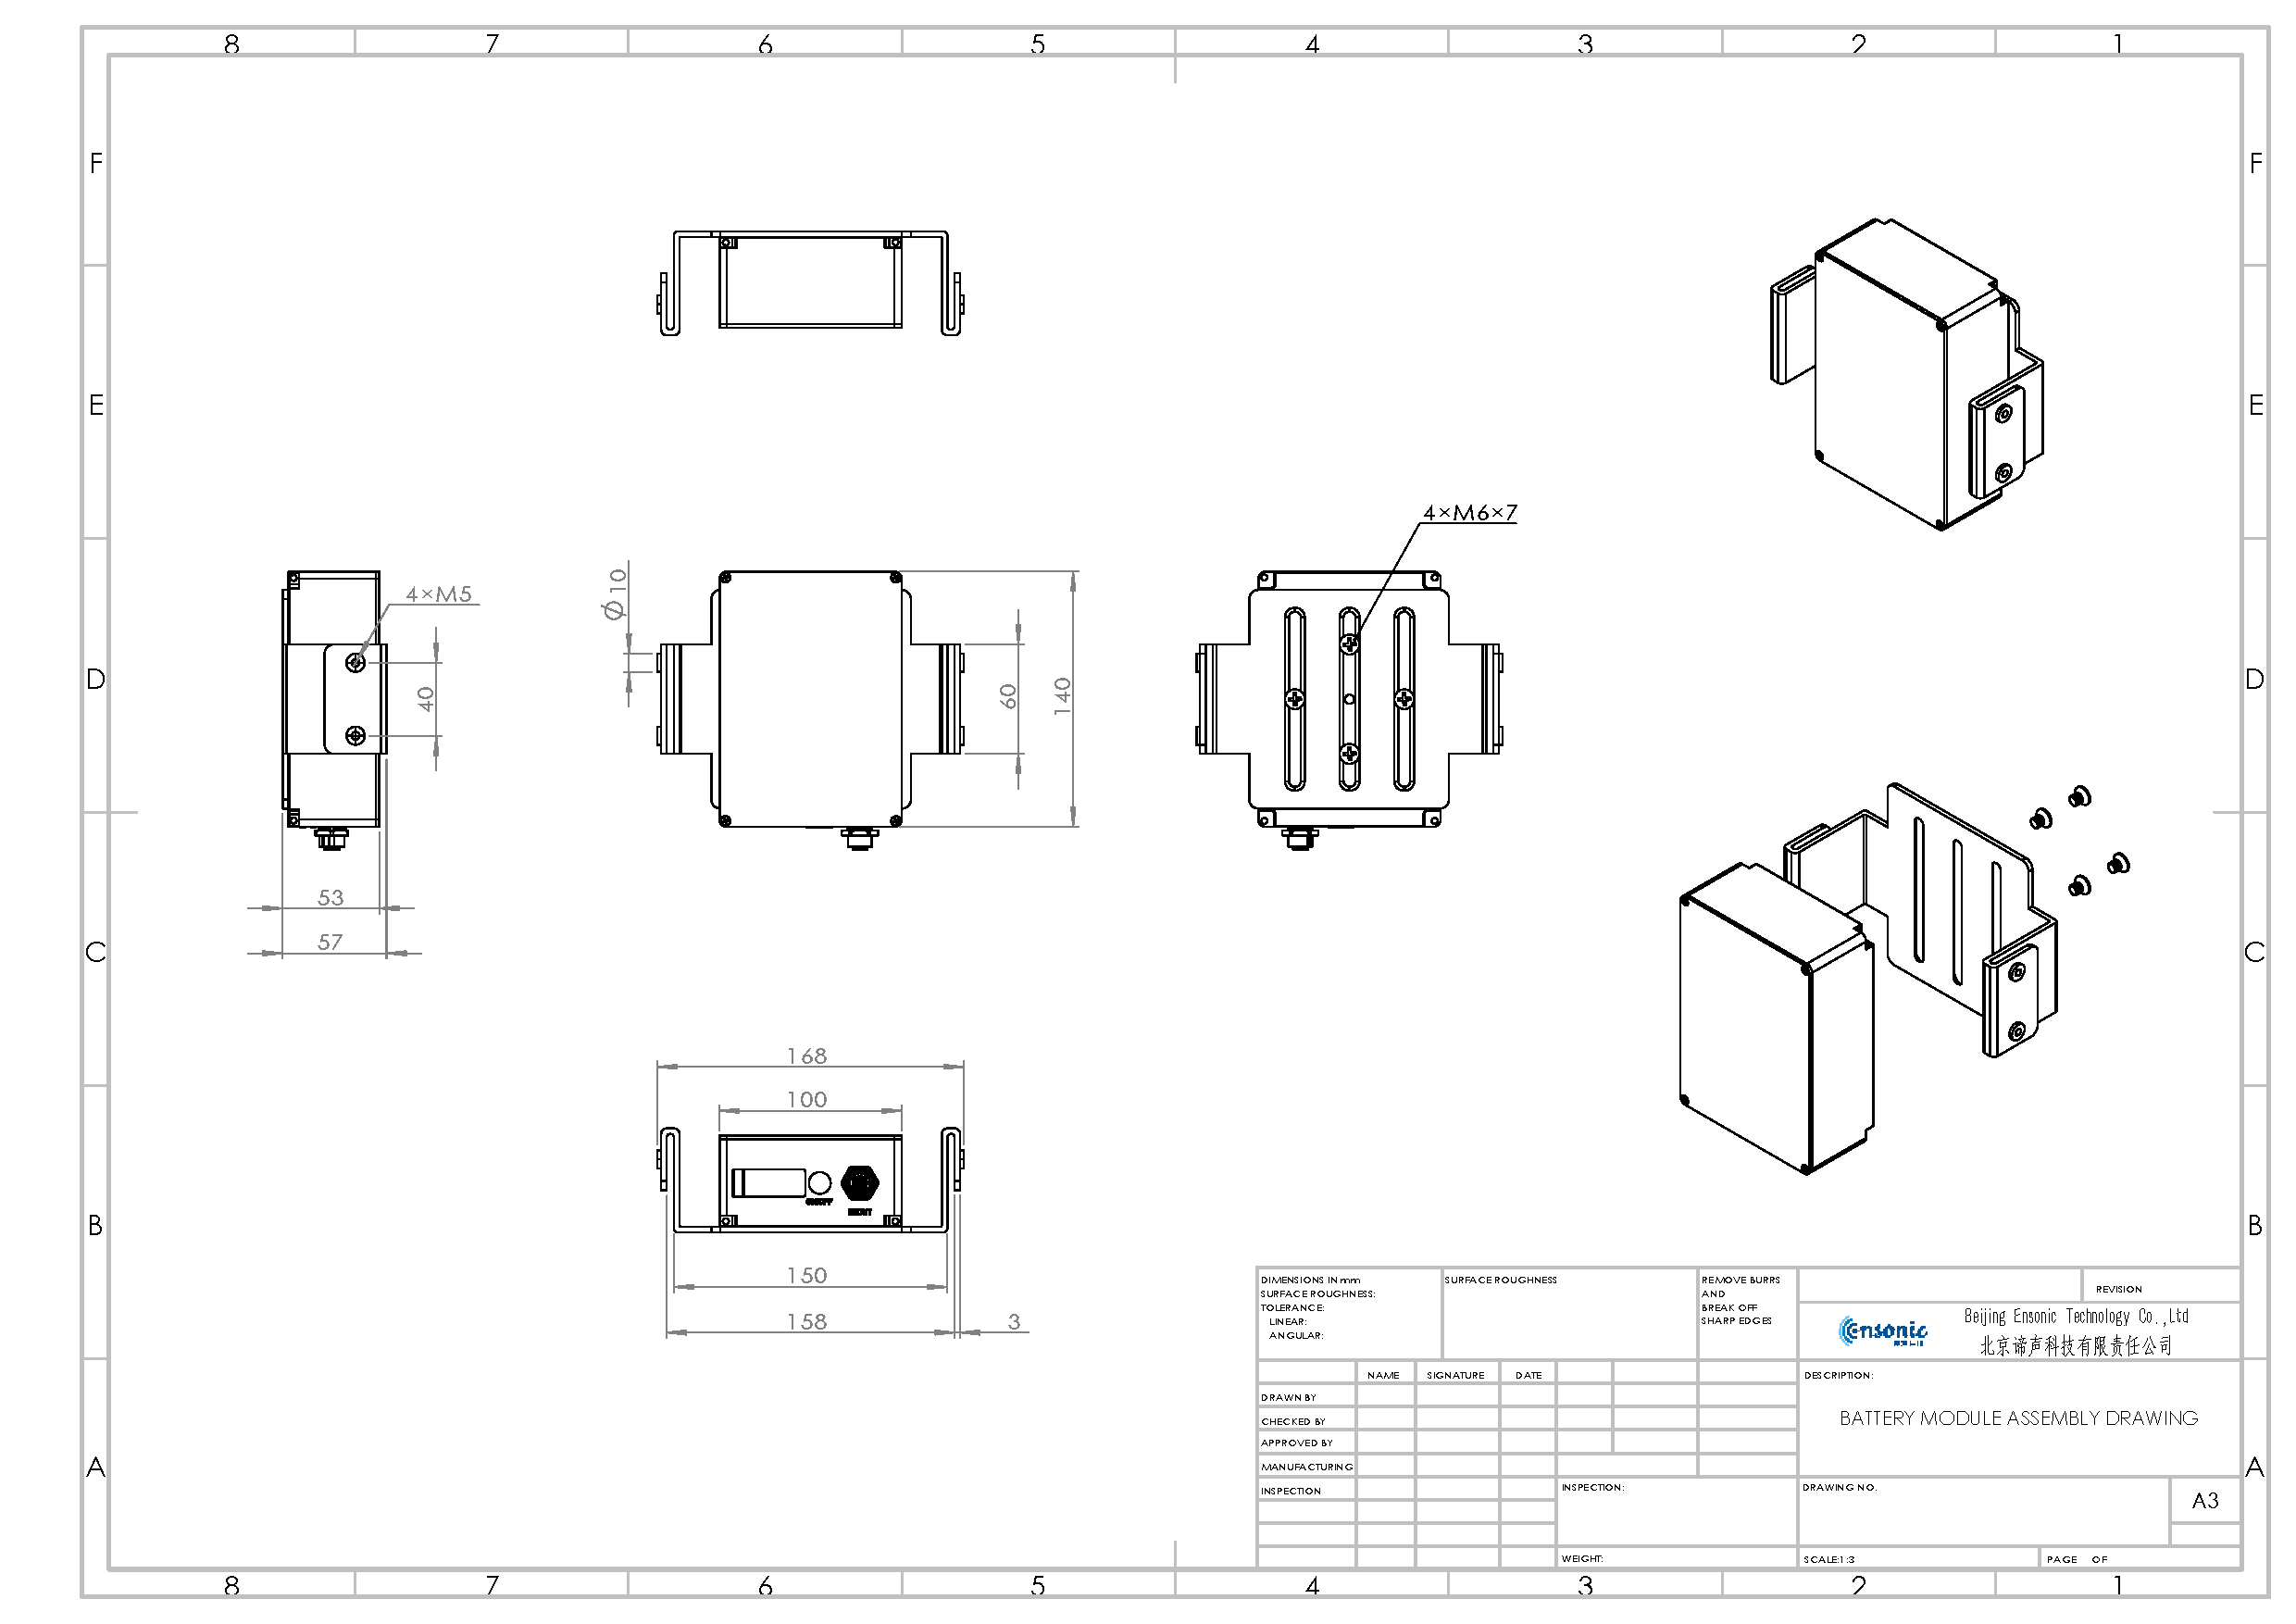
\includepdf[page={1-}, scale=0.75]{./电池装配体.pdf}
\subsubsection{Power Module}
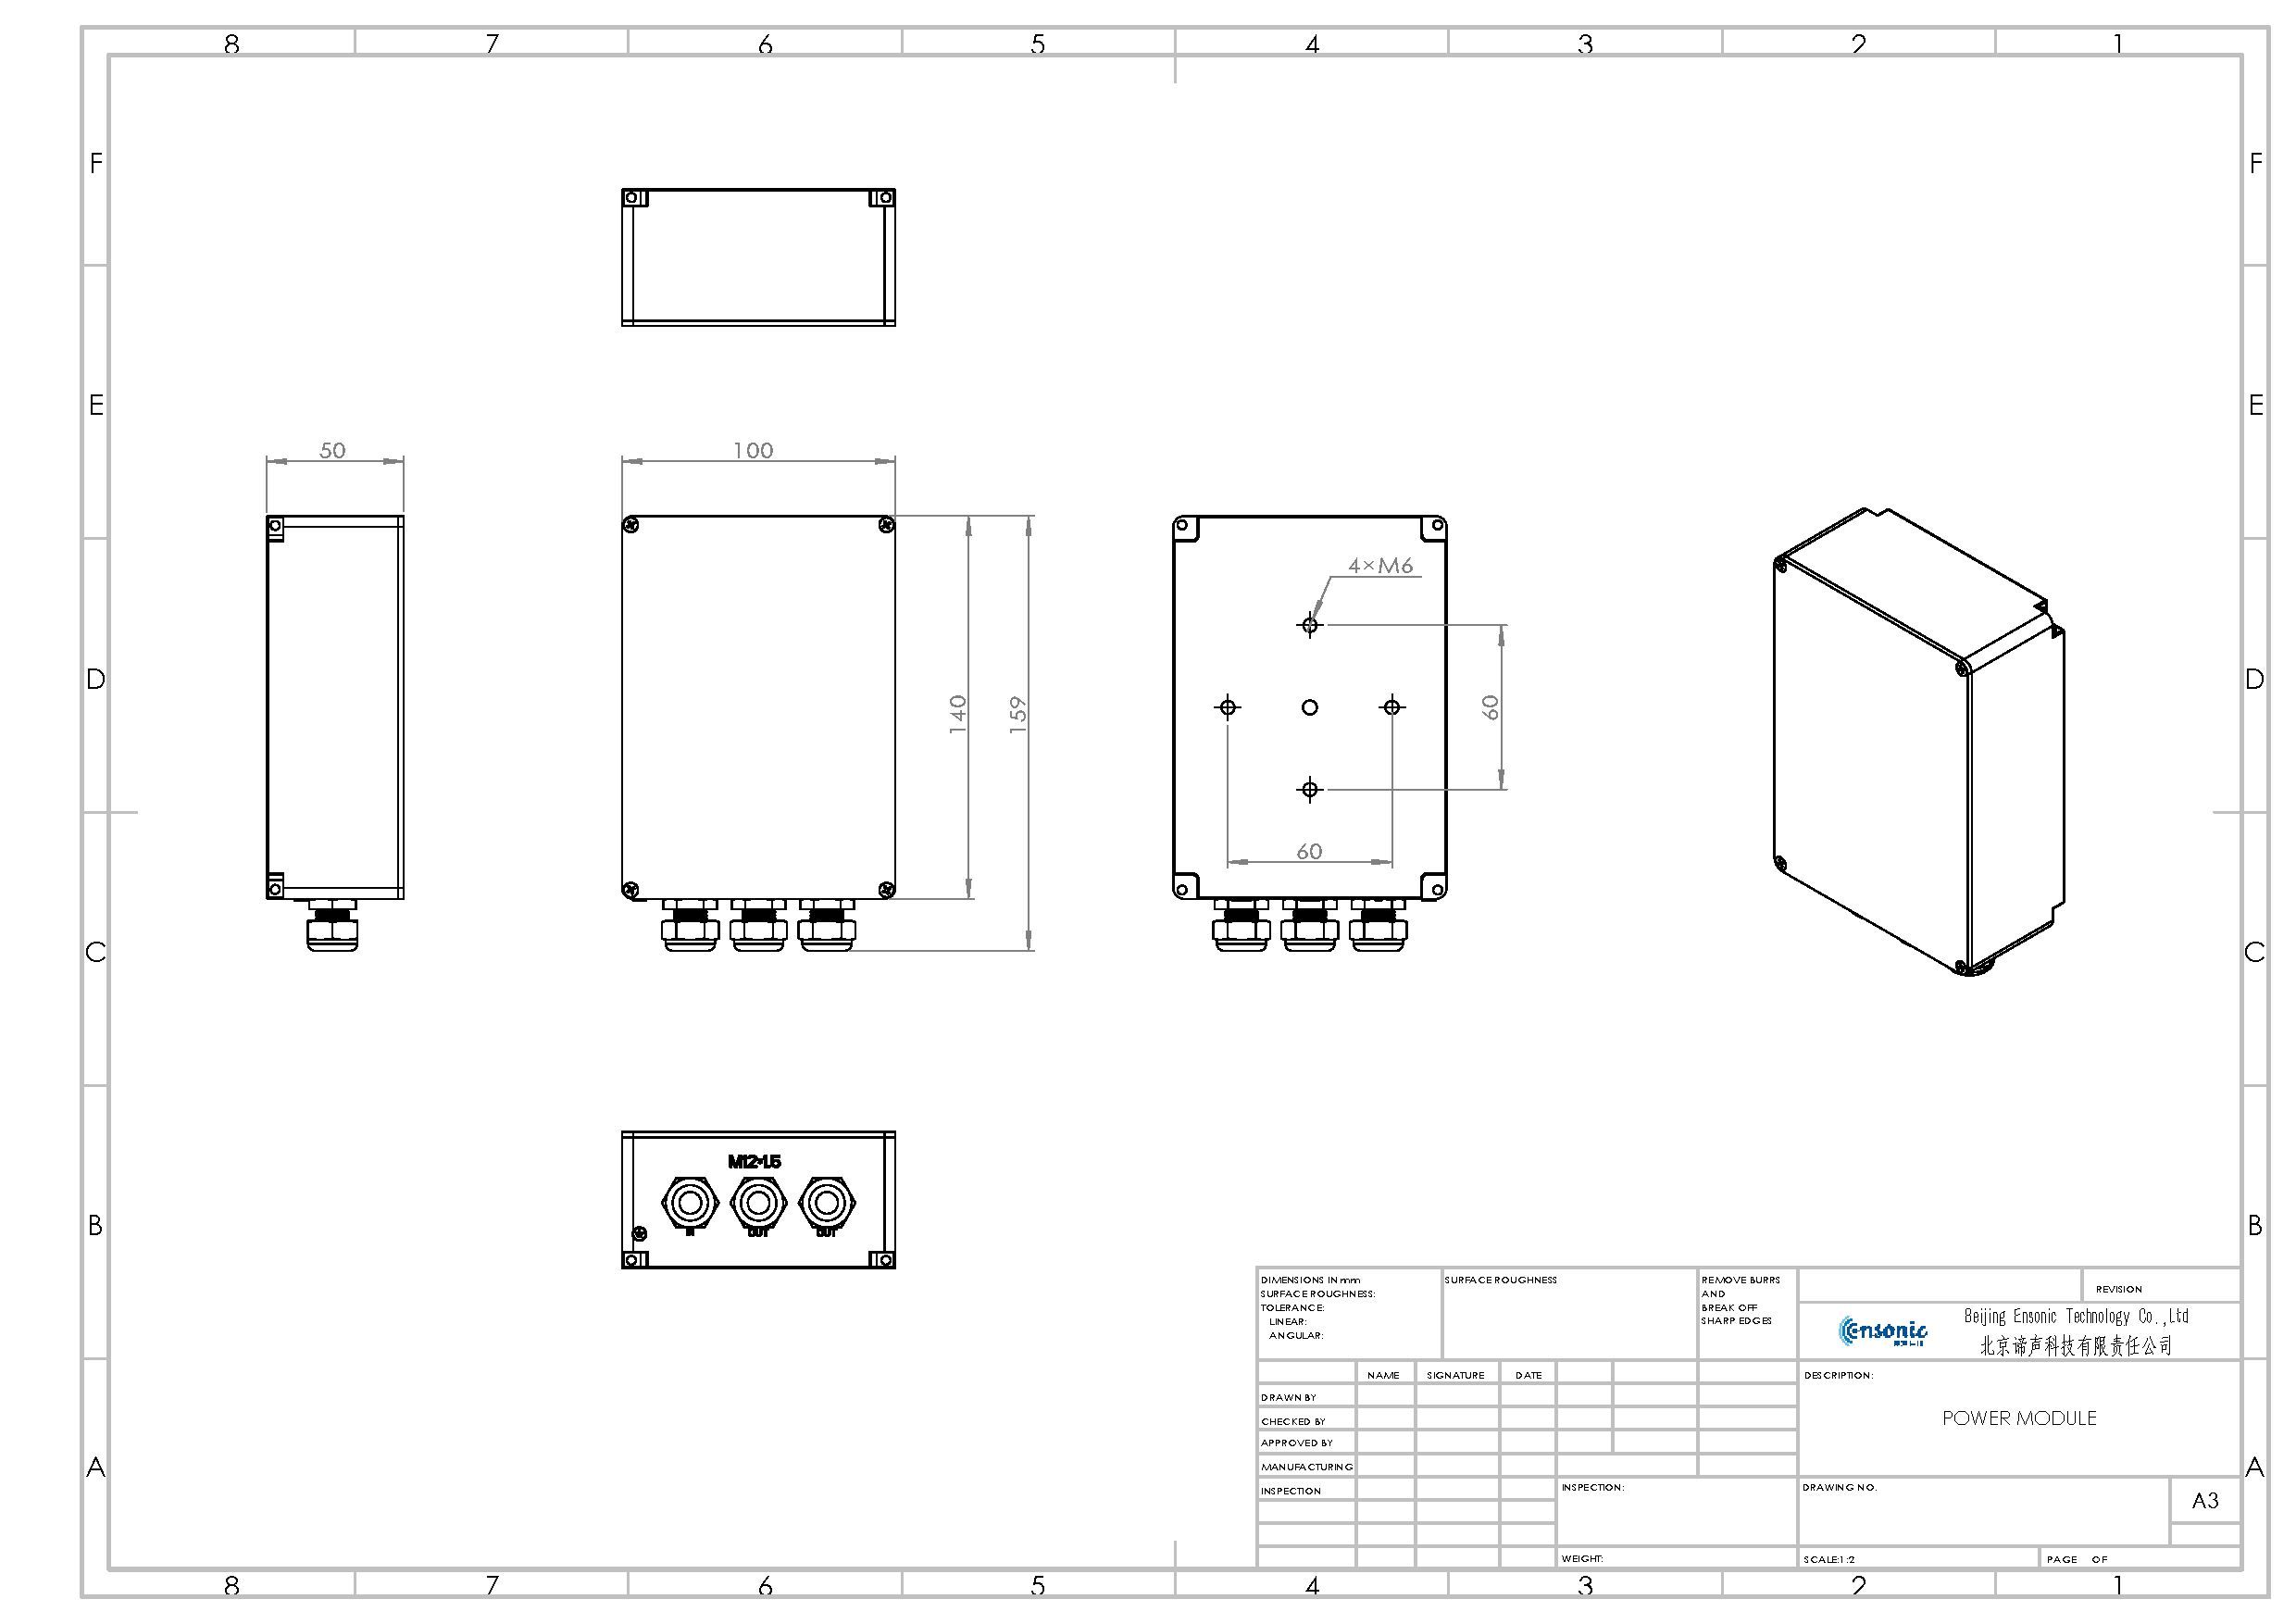
\includepdf[page={1-}, scale=0.75]{./电源装配体.pdf}
\subsubsection{Installation Mounting}
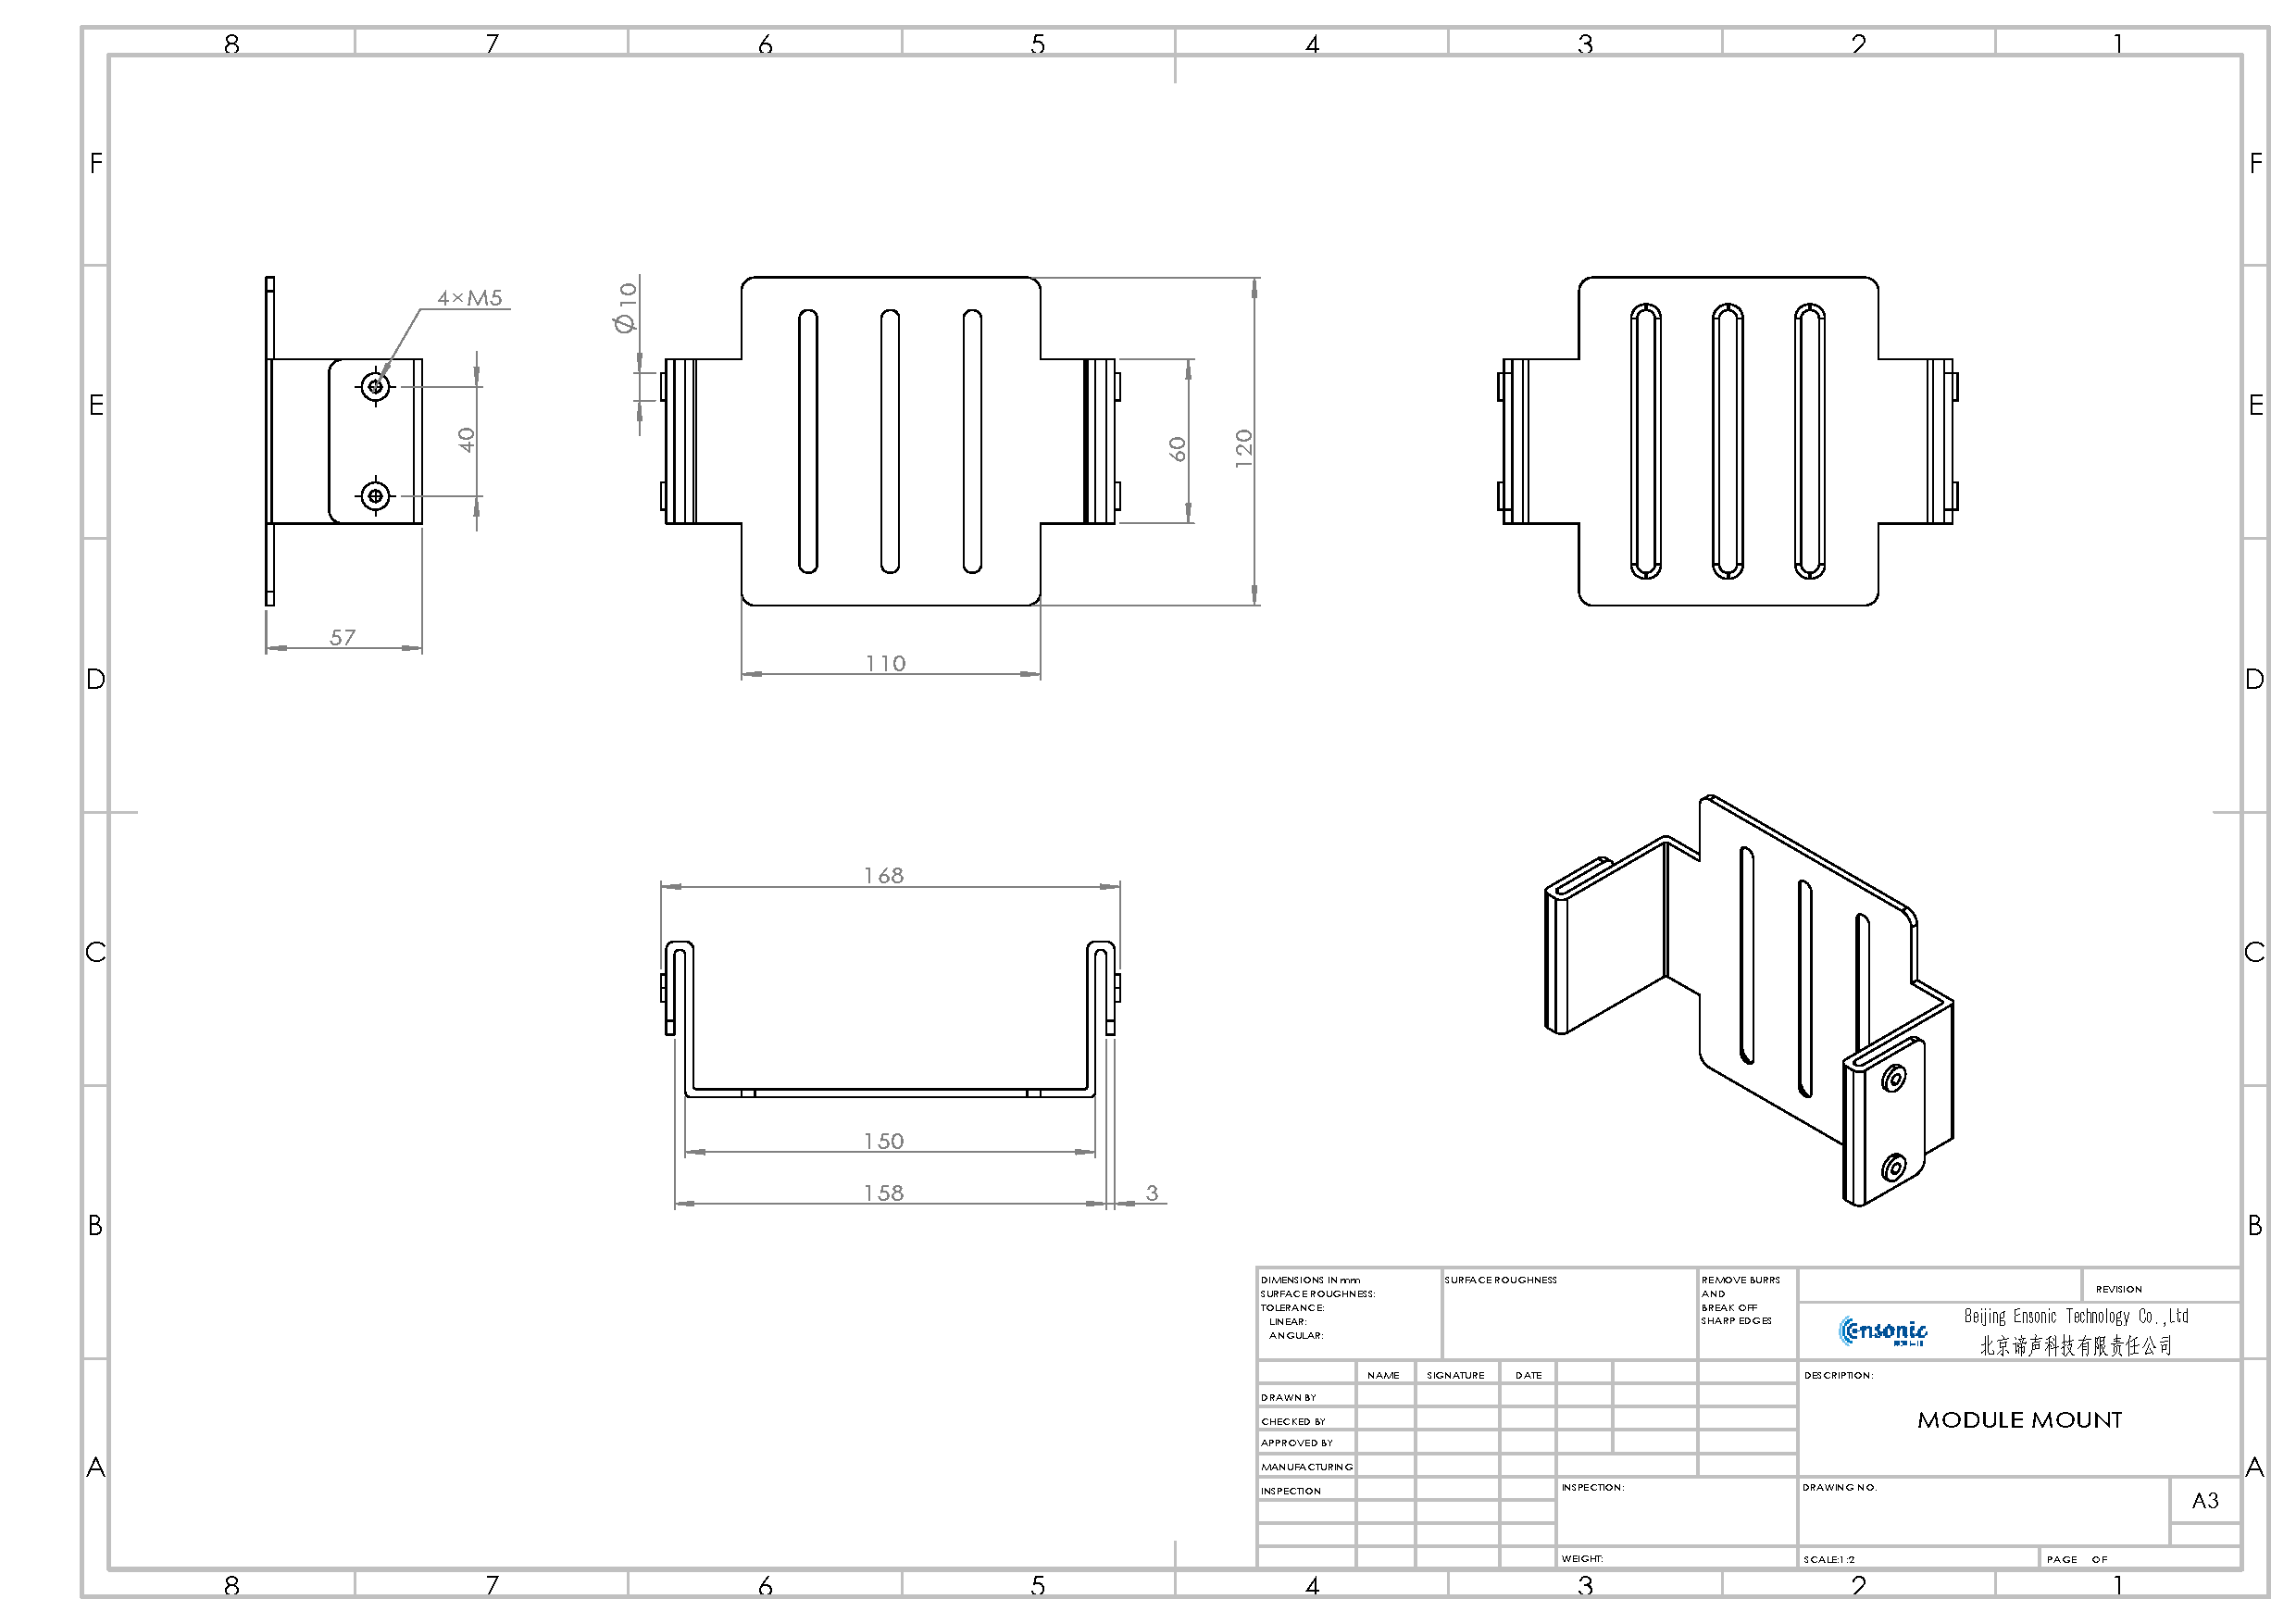
\includepdf[page={1-}, scale=0.75]{./安装支架.pdf}
\subsection{Installation with Battery Module}
\subsubsection{Installation Tools}
\begin{table}[htbp] % 表格浮动体,htbp 表示优先放置在当前位置
    \centering % 表格居中
    \caption{Tool list} % 表格标题
    \begin{tabular}{|c|c|c|} 
        \hline
        \toprule 
        Name & Usage & quantity\\
        \midrule % 
        Torque wrench & Tighten the bolts to the correct torque & 1 \\ \hline
        Scew driver & Assemble equipment mountings and plugs & 1 \\ \hline
        Markpen & Screw anti-loose mark & 1 \\ \hline
        \bottomrule % 底部粗线
    \end{tabular}
  \end{table}
\subsubsection{Installation Equipment and Accessories}
\begin{table}[htbp]
    \centering
    \caption{Equipment and Accessories List}
    \begin{tabular}{|c|c|c|}
        \hline
        \toprule
        Sample Picture & Name/Model & Quantity \\
        \midrule
        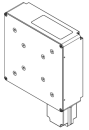
\includegraphics{RGME module.png}       & RGME Module                                             & 2 \\ \hline
        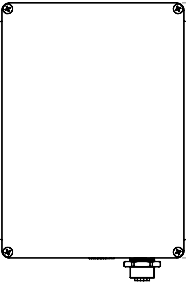
\includegraphics[width=0.08\textwidth]{Battery module.png}    & Battery Module                     & 2 \\ \hline       
%        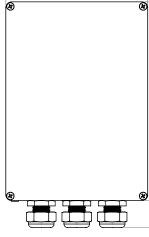
\includegraphics[width=0.1\textwidth]{Power module.png}      & Power Module                                            & 2 \\ \hline
        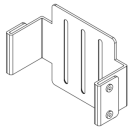
\includegraphics{Mounting.png}          & Installation Mounting                                   & 2 \\ \hline
        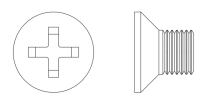
\includegraphics{M6x7.png}              & M6 × 7 cross countersunk head screw                     & 16 \\ \hline
        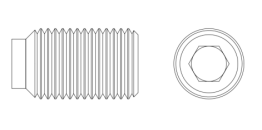
\includegraphics{M5x8.png}              &  M5 × 8 304 stainless steel POM nylon tip bolt           & 16 \\ \hline
        Working in Progress                     & Power Cable for Battery with WDZB-RVV 3*1mm$^2$             & 2 \\   \hline
    \end{tabular}
    \end{table}
\subsubsection{Pre-installation Preparation}
\begin{enumerate}
    \item Onsite installation position confirmation, RGME module and Power/Battery module are installed on the back of the decorative panel of the car near to Door 1 and Door 5 on the same side.
    \item Select the RGME module and Installation Mounting from the equipment list, and fix them with M6 × 7 cross countersunk head screw. The relative position can be adjusted up and down according to the mutual influence of the actual installation positions on site.\\
    \begin{center}
        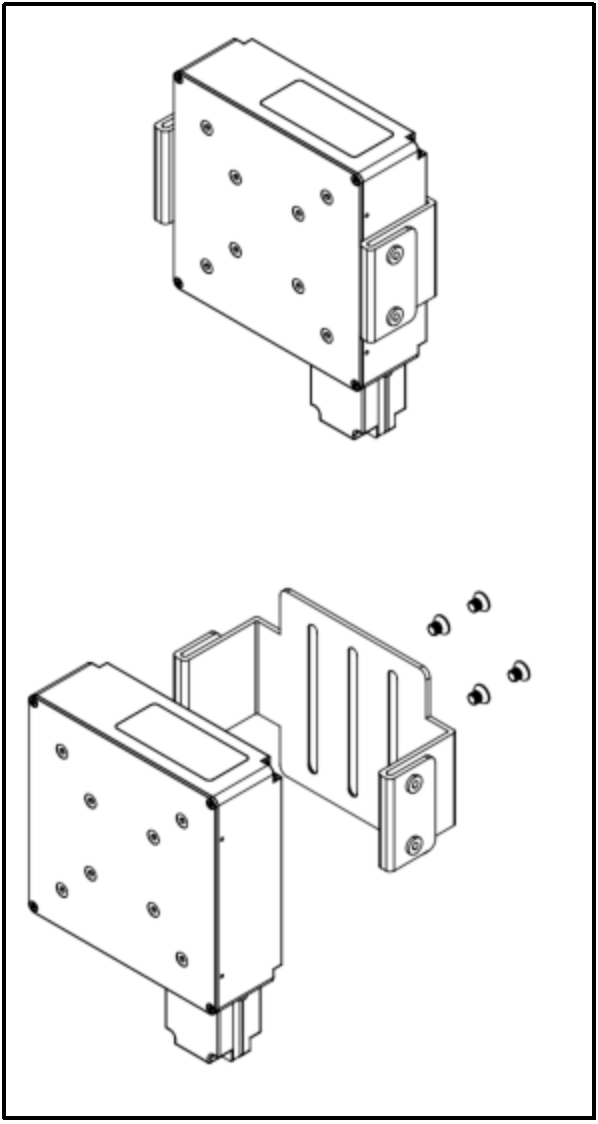
\includegraphics[width=0.2\textwidth]{RGME Mounting.png}
    \end{center}
    \item Select the Battery module and Installation Mounting from the equipment list, and fix them with M6 × 7 cross countersunk head screw. The relative position can be adjusted up and down according to the mutual influence of the actual installation positions on site.\\     
    \begin{center}
        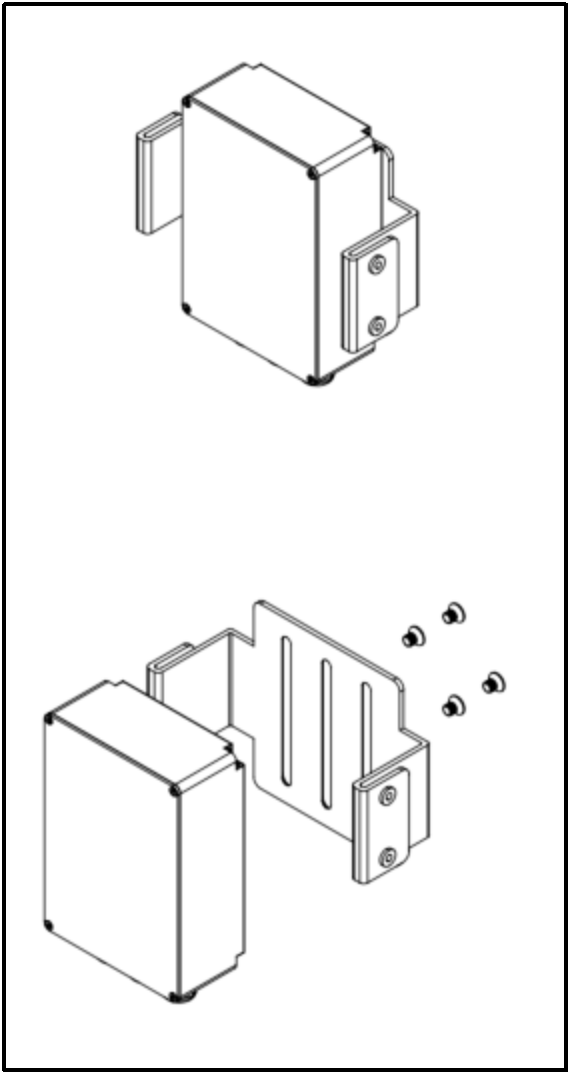
\includegraphics[width=0.2\textwidth]{Battery Mounting.png}
    \end{center}
    \item Tighten the screws with a torque of 10 N·m, and use a marker pen to draw a line as a mark to prevent loosening.\\
    \begin{center}
        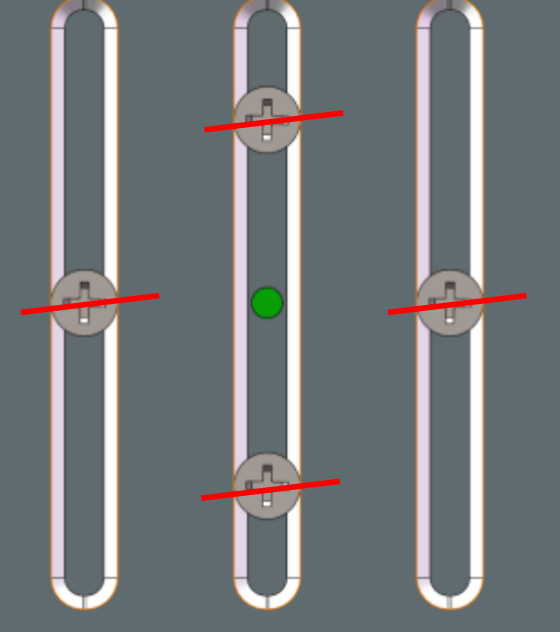
\includegraphics[width=0.3\textwidth]{Mark1.png}
    \end{center}
\end{enumerate}
\subsubsection{Installation on Car}
\begin{enumerate}
    \item Pick up the RGME module with the mounting, put it into the dedicated position inside the structure beam on car behind the decoration panel near door 1.\\
    \begin{center}
        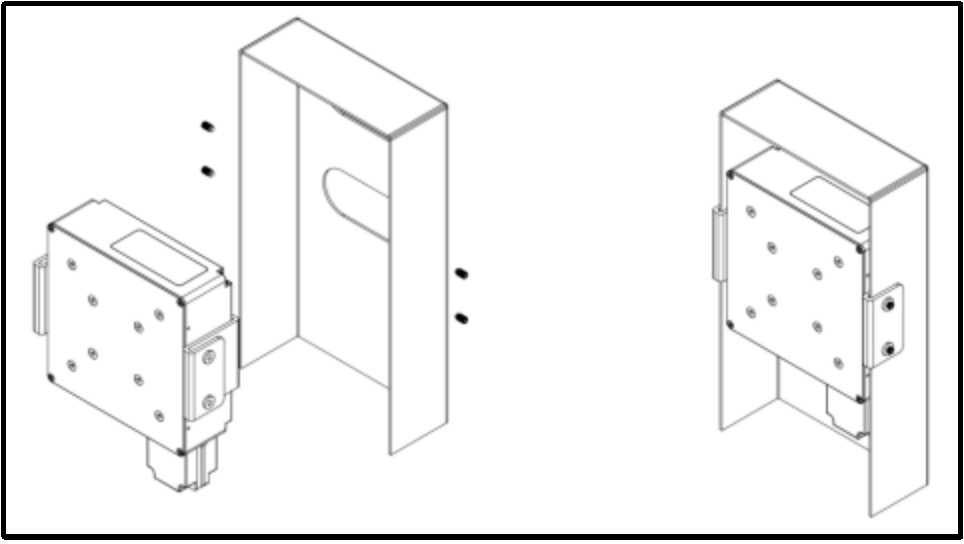
\includegraphics[width=0.5\textwidth]{RGME ready.png}
    \end{center}
    \item Screw it with M5 × 8 304 stainless steel POM nylon tip bolt to the structure beam, and tighten it with a torque of 6.5 N·m.\\
    \item Use a marker pen to draw a line as a mark to prevent loosening.\\
    \begin{center}
        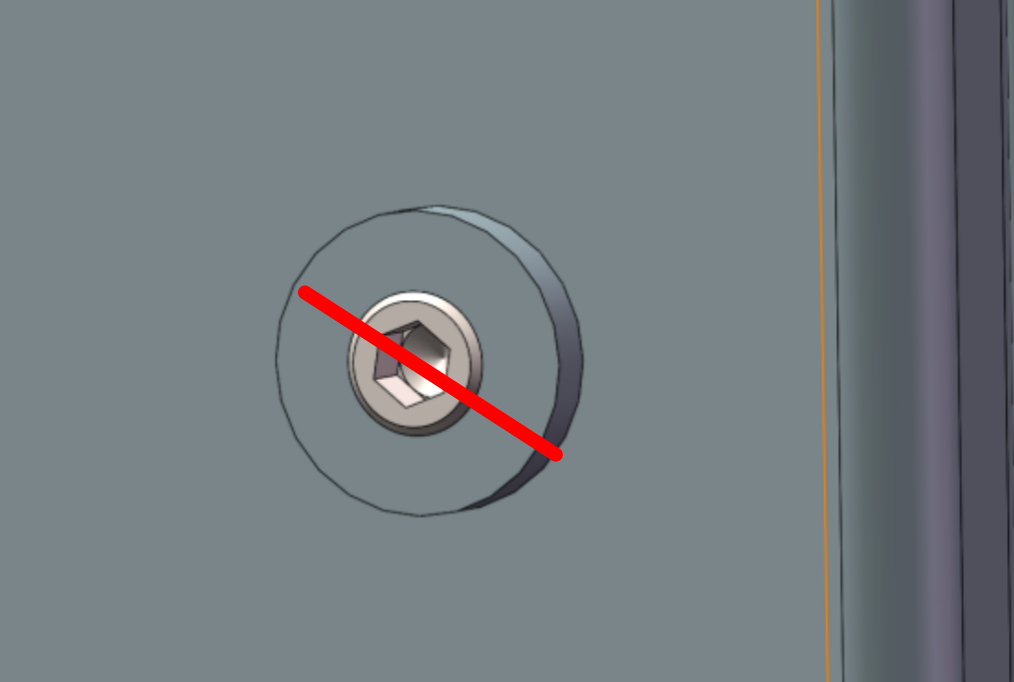
\includegraphics[width=0.5\textwidth]{Mark2.png}
    \end{center}
    \item Pick up the Battery module with the mounting, put it into the dedicated position inside the structure beam on car behind the decoration panel near door 1. And also screw it with the same torque and line mark it.\\
    \begin{center}
        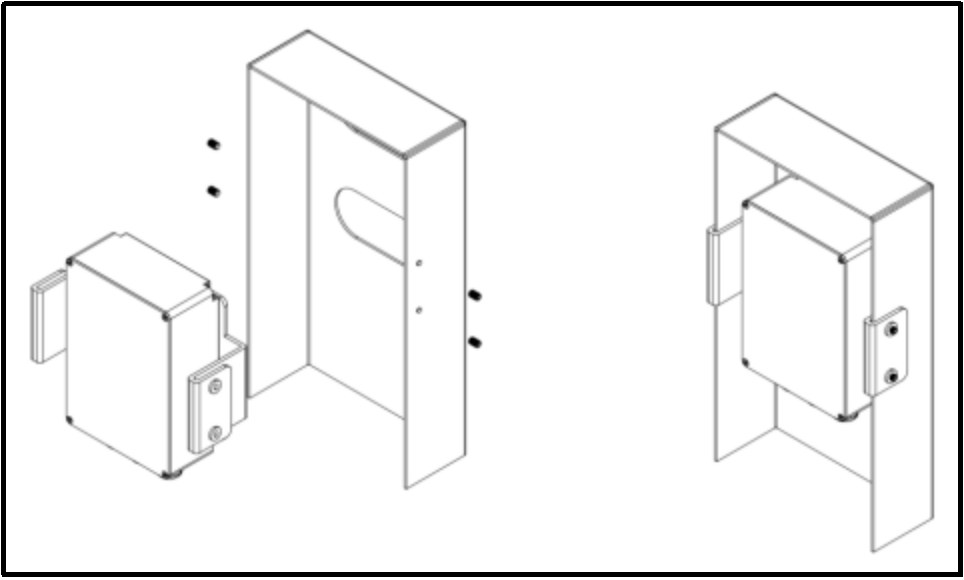
\includegraphics[width=0.5\textwidth]{Battery ready.png}
    \end{center}
    \item Connect the power cable to the RGME module and Battery module.\\
    \item Repeat the above steps for the installation of RGME module and Battery module on the other side of the car.\\
    \item When tightening all the screws, use Loctite 222 thread locking adhesive to prevent the screws from loosening.\\
\end{enumerate}
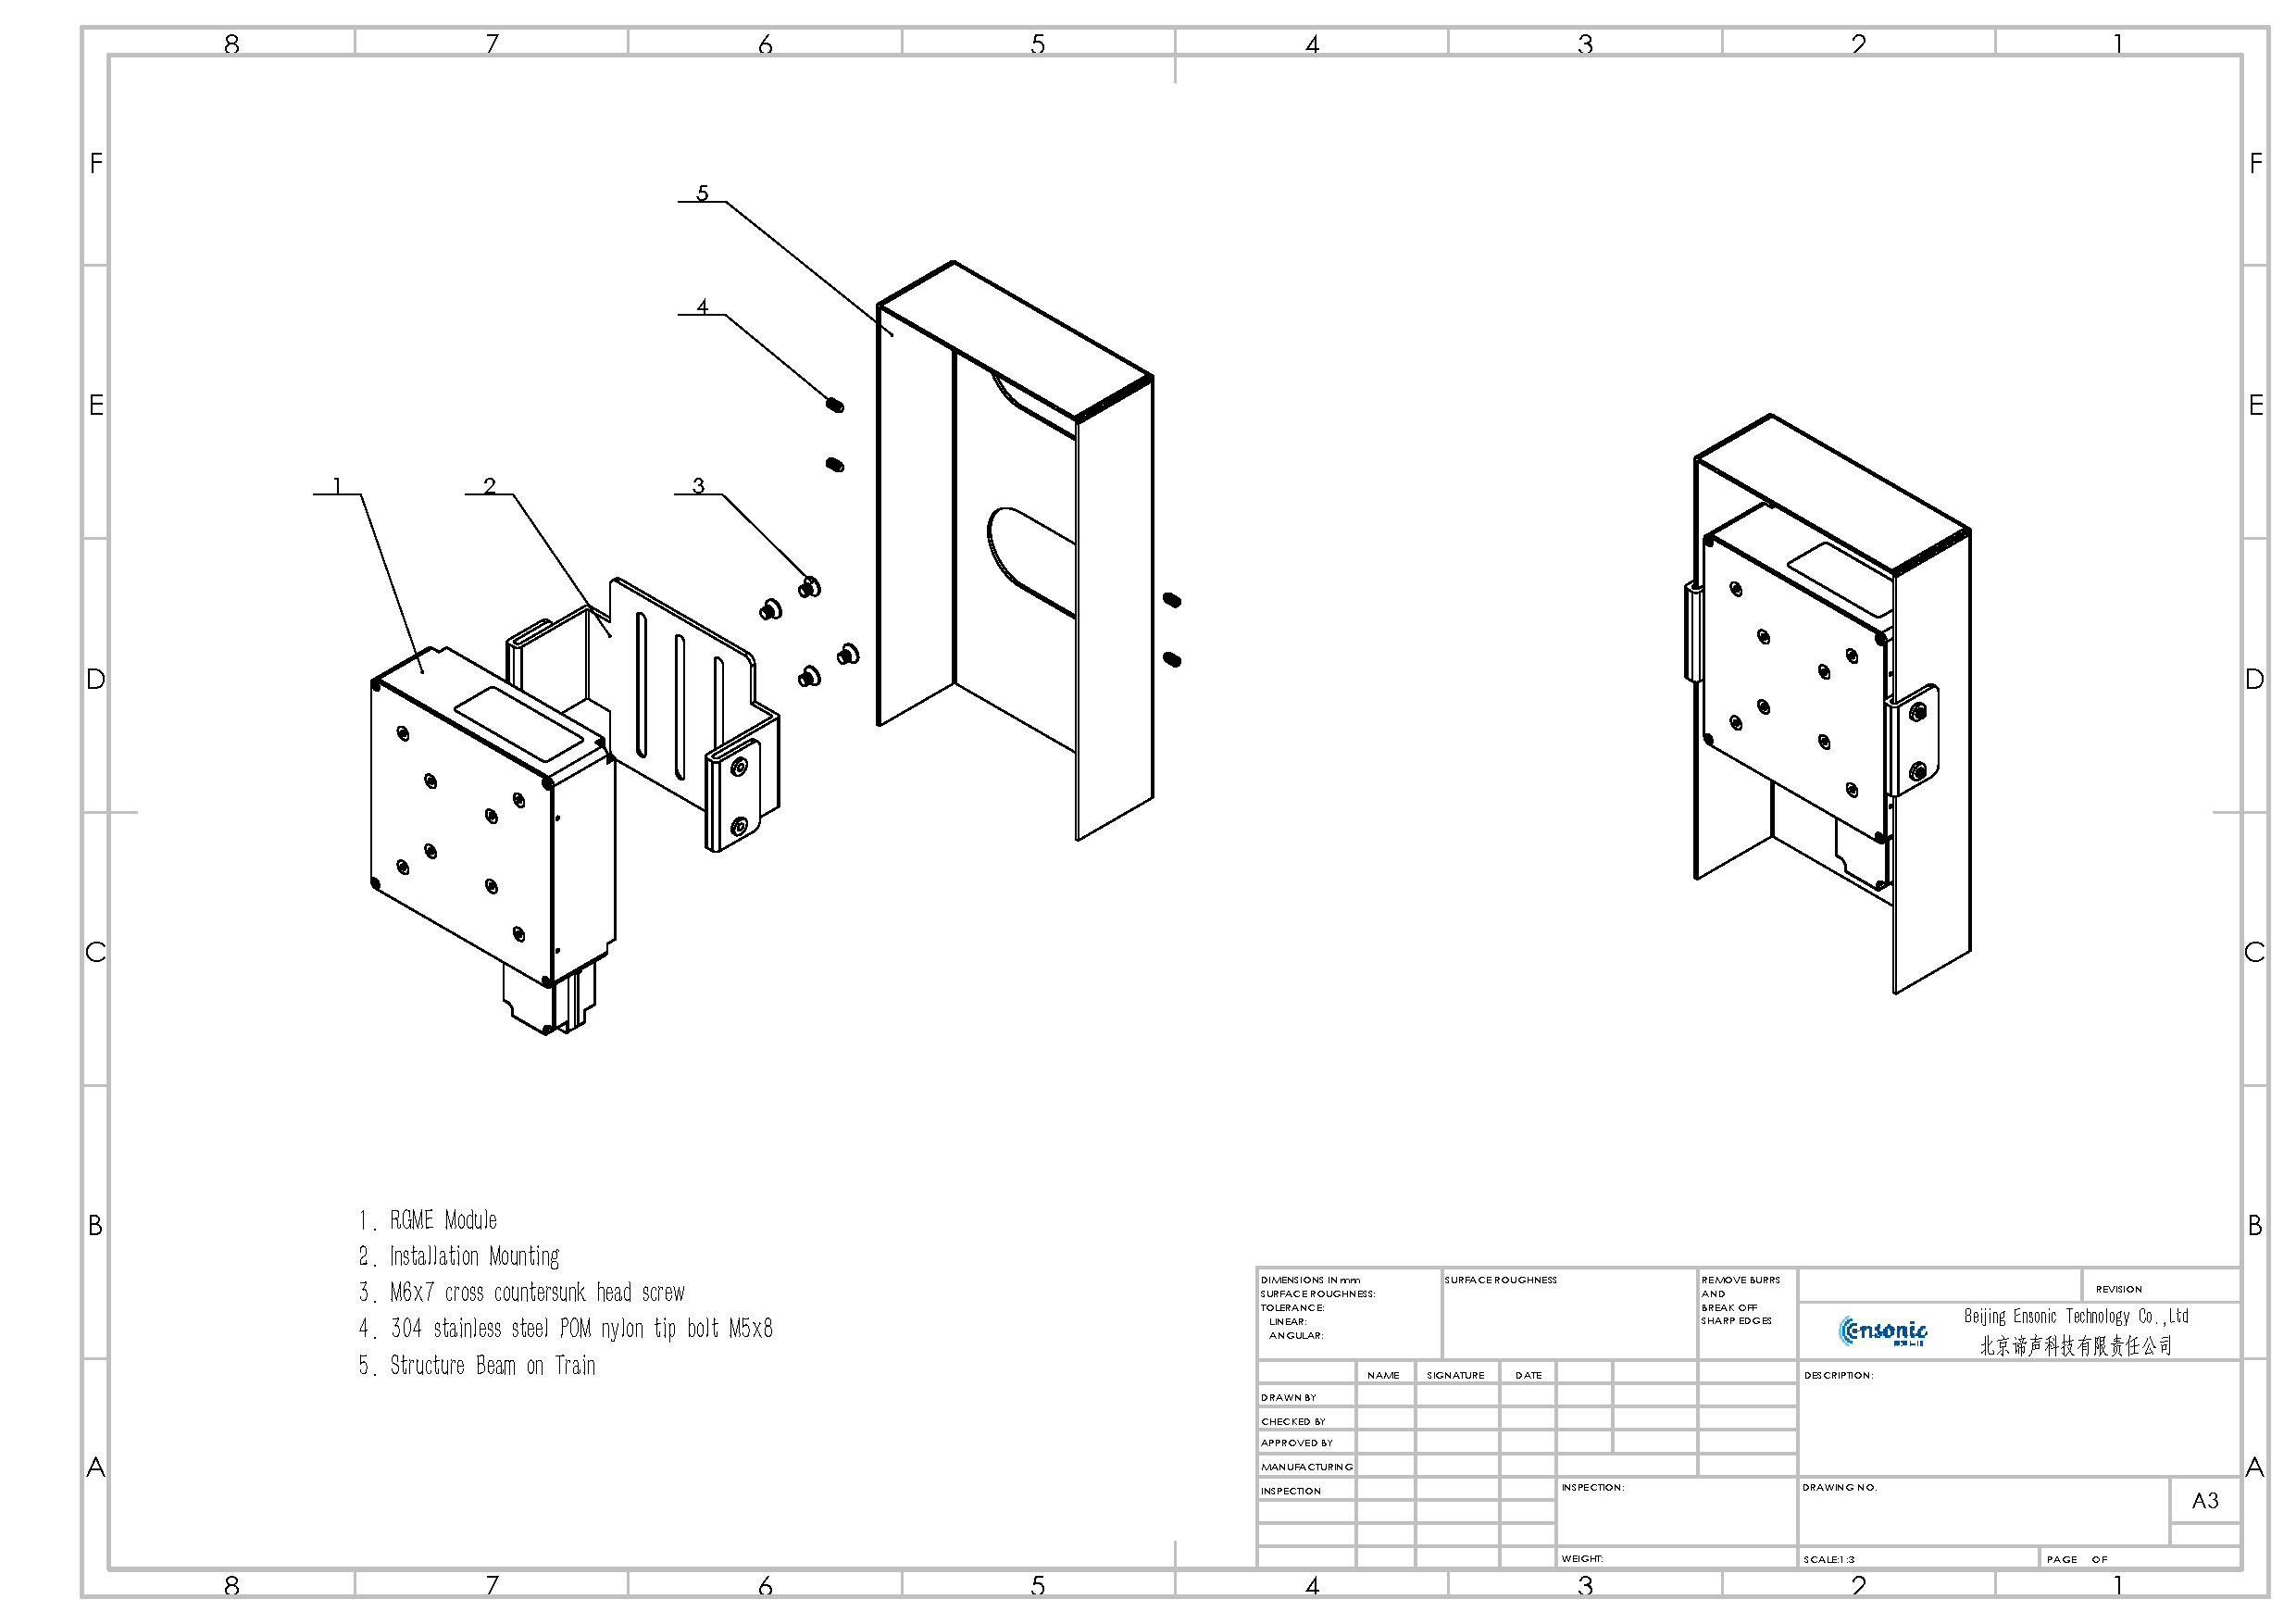
\includepdf[page={1-}, scale=1]{./现场安装示意图_声纹终端.pdf}
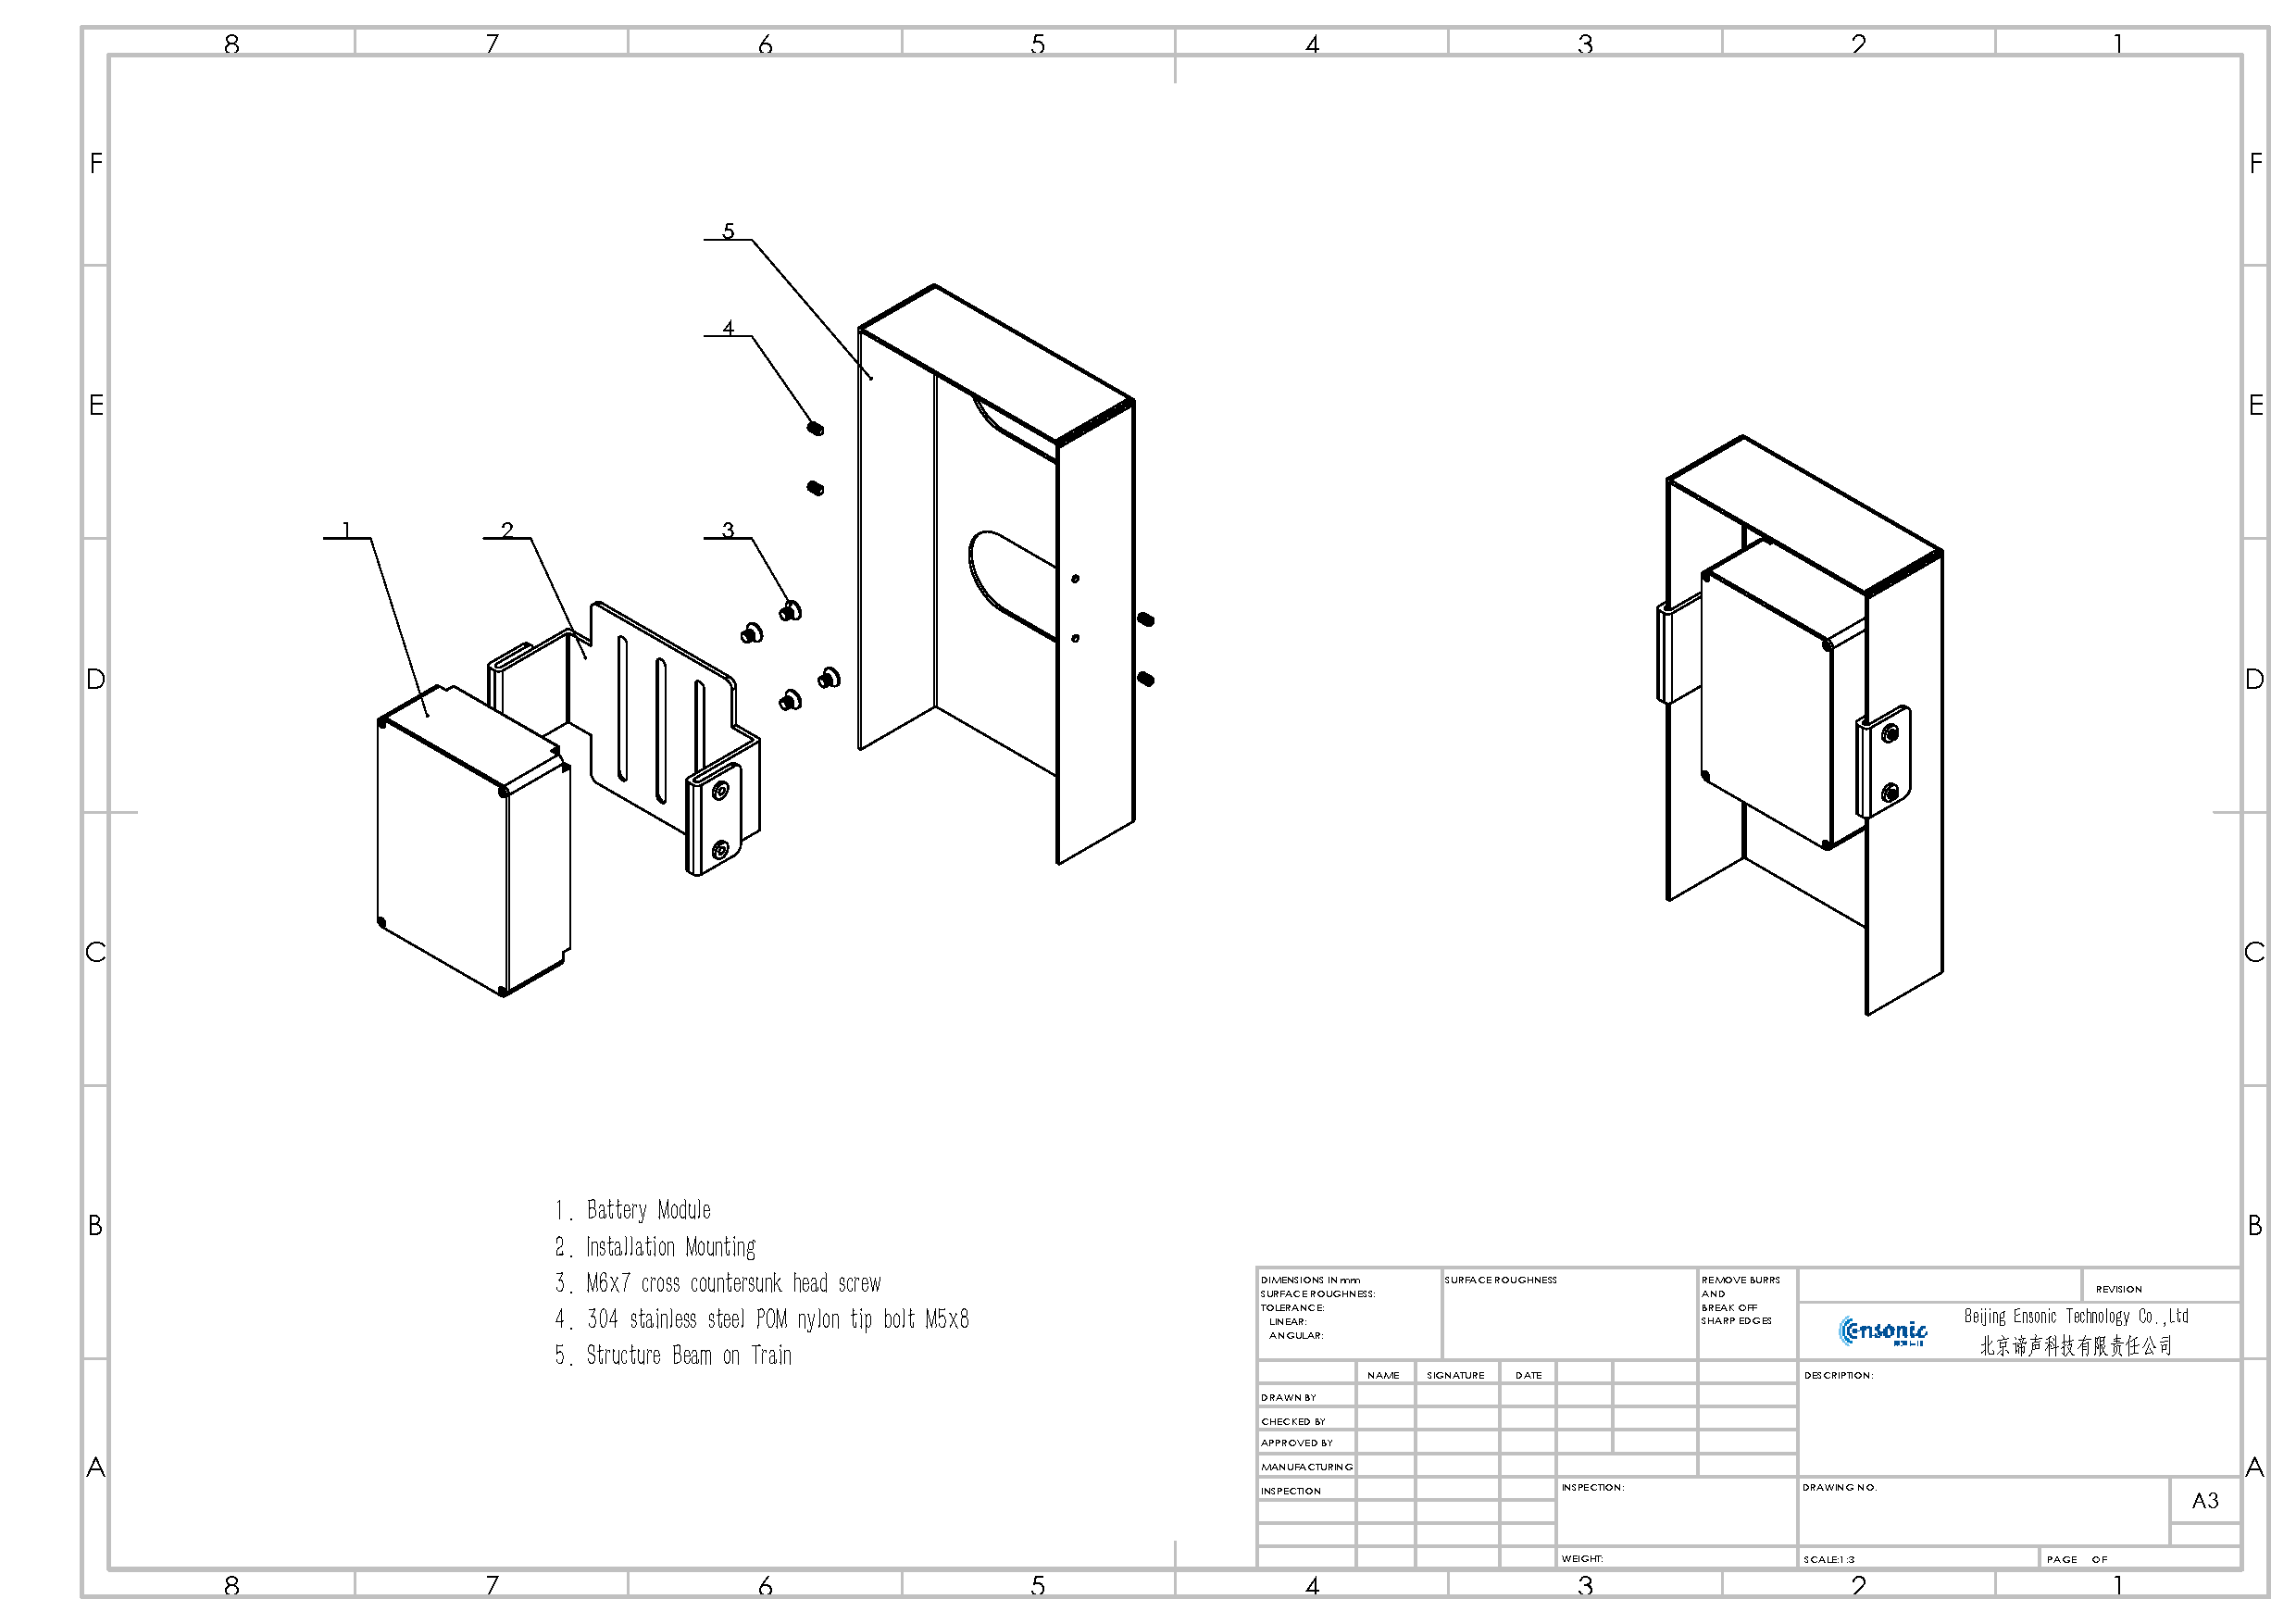
\includepdf[page={1-}, scale=1]{./现场安装示意图_电池.pdf}
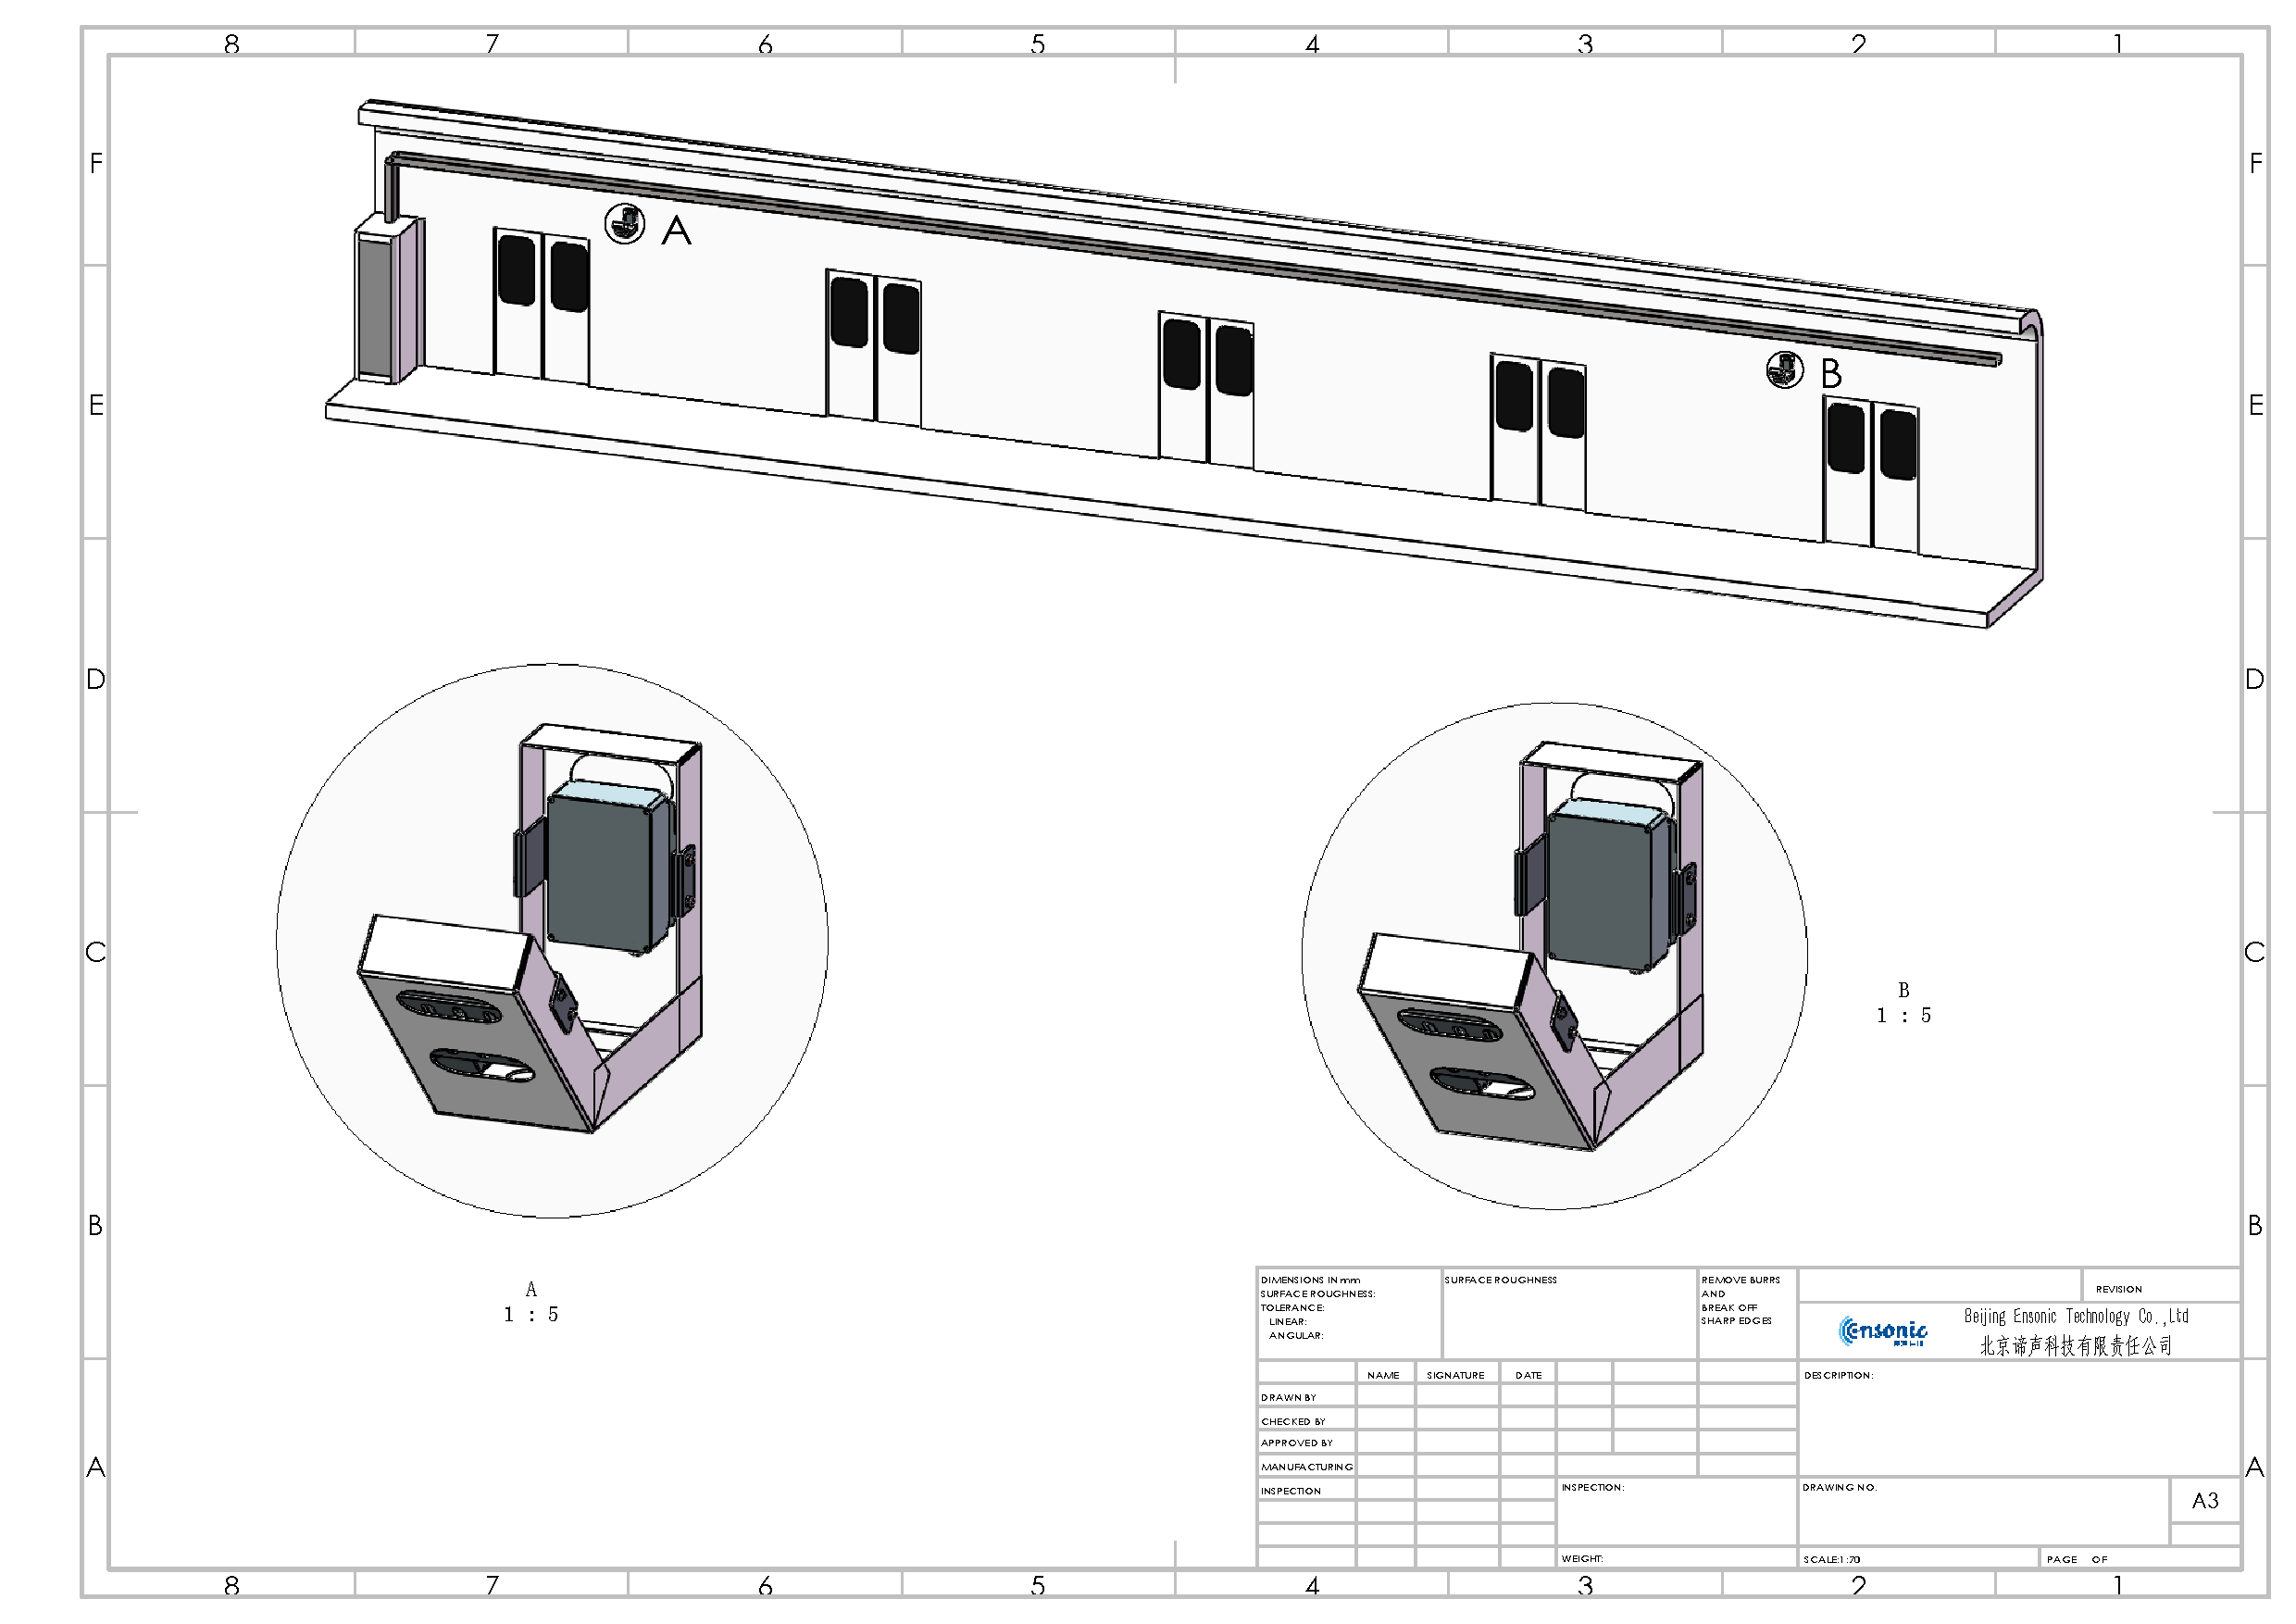
\includepdf[page={1-}, scale=0.75]{./电池安装_布局示意图.pdf}
\subsection{Installation with Power Module}
\subsubsection{Installation Tools}
\begin{table}[htbp] % 表格浮动体,htbp 表示优先放置在当前位置
    \centering % 表格居中
    \caption{Tool list} % 表格标题
    \begin{tabular}{|c|c|c|} 
        \hline
        \toprule 
        Name & Usage & quantity\\
        \midrule % 
        Torque wrench & Tighten the bolts to the correct torque & 1 \\ \hline
        Scew driver & Assemble equipment mountings and plugs & 1 \\ \hline
        Wire stripper & Strip the power cable & 1 \\ \hline
        Crimping plier & Crimp the power cable with the cable gland & 1 \\ \hline
        Diagonal plier & Cut the power cable & 1 \\ \hline
        Electric soldering iron & Solder the power cable & 1 \\ \hline
        Solder wire & Solder the power cable & 1 \\ \hline
        Soldering flux & Solder the power cable & 1 \\ \hline
        Heat gun & Heat shrink the power cable protection & 1 \\ \hline
        Markpen & Screw anti-loose mark & 1 \\ \hline
        \bottomrule % 底部粗线
    \end{tabular}
\end{table}
\subsubsection{Installation Equipment and Accessories}
\clearpage
\begin{table}[H]
    \centering
    \caption{Equipment and Accessories List}
    \begin{tabular}{|c|c|c|}
        \hline
        \toprule
        Sample Picture & Name/Model & Quantity \\
        \midrule
        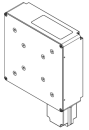
\includegraphics{RGME module.png}       & RGME Module                                             & 2 \\ \hline
%        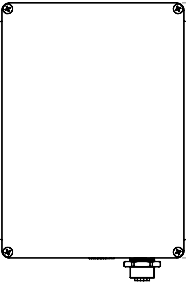
\includegraphics[width=0.08\textwidth]{Battery module.png}    & Battery Module                     & 2 \\ \hline       
        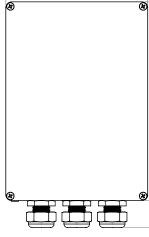
\includegraphics[width=0.08\textwidth]{Power module.png}      & Power Module                                            & 2 \\ \hline
        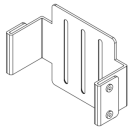
\includegraphics{Mounting.png}          & Installation Mounting                                   & 2 \\ \hline
        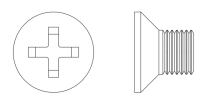
\includegraphics{M6x7.png}              & M6 × 7 cross countersunk head screw                     & 16 \\ \hline
        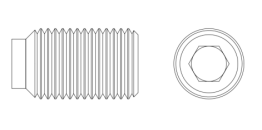
\includegraphics{M5x8.png}              &  M5 × 8 304 stainless steel POM nylon tip bolt           & 16 \\ \hline
        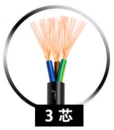
\includegraphics{Power cable.png}                    & Power Cable WDZB-RVV 3*1mm$^2$             & 30 meters \\   \hline
        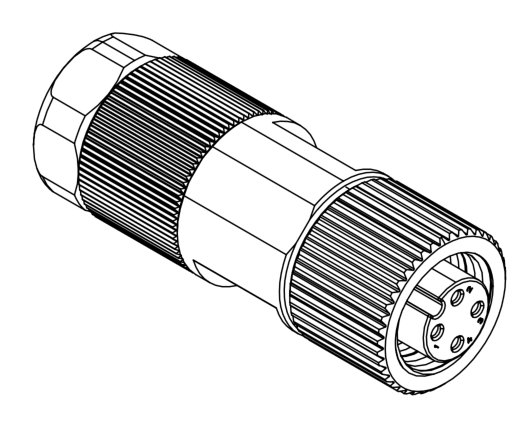
\includegraphics[width=0.15\textwidth]{A-code.png}                    & A-code Plug                                            & 2 \\ \hline
        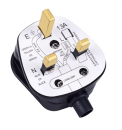
\includegraphics{Plug.png}                  & Plug for AC220V                                      & 1 \\ \hline
        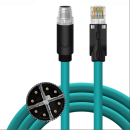
\includegraphics{X-code.png}                    & X-code Plug for read data from RGME offline       & 1 \\ \hline
        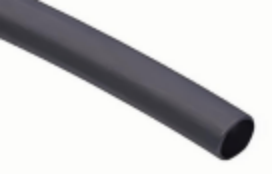
\includegraphics[width=0.15\textwidth]{热缩管.png}                    & $\varnothing$ 3mm Heat shrink tube               & 0.5 meters\\ \hline
        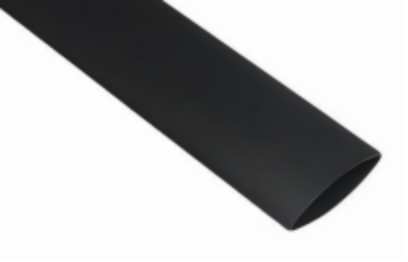
\includegraphics[width=0.15\textwidth]{线缆保护管.png}                 & Cable protection tube                         & 30 meters\\ \hline
    \end{tabular}
\end{table}
\subsubsection{Pre-installation Preparation}
\begin{enumerate}
    \item Onsite installation position confirmation, RGME module and Power/Battery module are installed on the back of the decorative panel of the car near to Door 1 and Door 5 on the same side.
    \item Confirm the AC220V power socket position.
    \begin{center}
        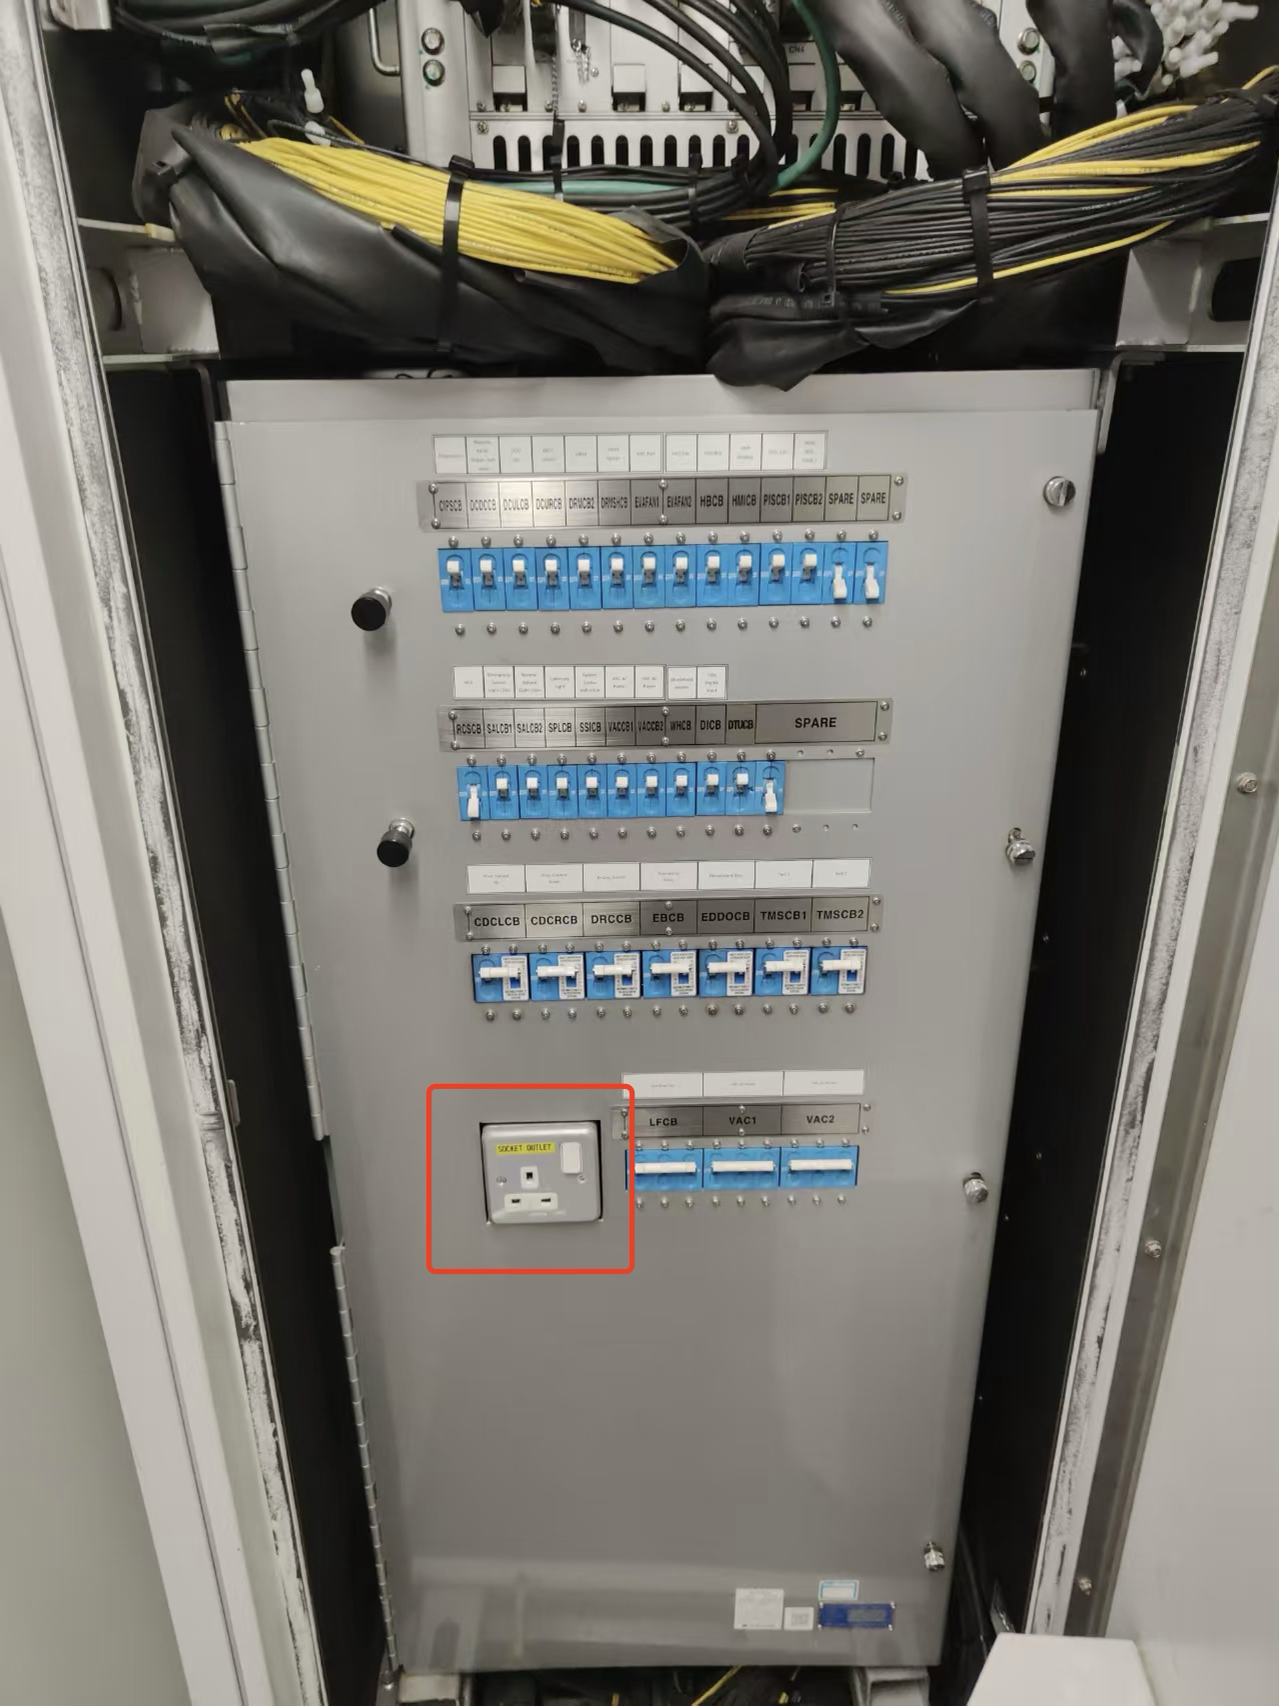
\includegraphics[width=0.5\textwidth]{Power socket.jpg}
    \end{center}
    \item Verify the cable laying path and the grooves involved in the cable laying path, and measure and estimate the length of each cable.
    \begin{enumerate}
        \item The cable length from the power socket to the Power module.
        \item The cable length from the Power module to the RGME module 1.
        \item The cable length from the Power module to the RGME module 2.
    \end{enumerate}
    \item Intercept the cable according to the measured length and paste the cable labels.
    \item Cable protection measures: intercepted cable cover black cable protection tube.
    \item Use scew driver to open the Power module cover, insert the corresponding cable from the gland hole and follow the instructions below to connect to the power connector.
    \begin{figure}[H]
        \centering
        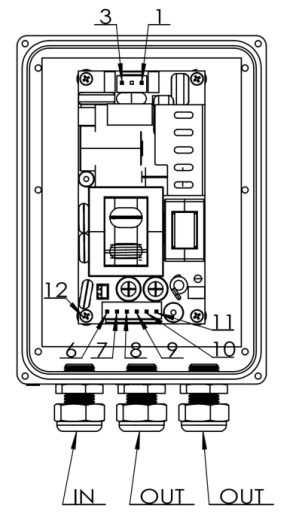
\includegraphics{Power module open B.png}
        \caption{inside view of Power module}
    \end{figure}
    \begin{table}[htbp]
        \centering
        \caption{Power module pin definition}
        \begin{tabular}{|p{2cm}|p{3cm}|p{2cm}|p{6cm}|}
            \hline
            \toprule
            PIN No. & Function & Core Color & Descrption \\
            \midrule
            1 & AC-N & RED & AC220V power supply input, cable through the IN gland\\ \hline
            3 & AC-L & BLACK & AC220V power supply input, cable through the IN gland\\ \hline
            6,7,8 & DC12V- & BLACK & DC12V power supply output, 2 cables through the OUT glands, seperatedly supply to 2 RGME module \\ \hline
            9,10,11 & DC12V+ & RED & DC12V power supply output, 2 cables through the OUT glands, seperatedly supply to 2 RGME module \\ \hline
            12 & PE & WHITE & PE cable, 3 cables all connect to PIN 12\\ \hline
            \bottomrule
        \end{tabular}
    \end{table}
    \item According to the above table, connect the power cable to the Power module. The power cable is connected to the Power module through the IN gland hole, and the other end is connected to the AC220V power socket. The RGME modules are connected to the Power module through the OUT gland holes.
    \begin{table}
        \centering
        \caption{A-code Plug pin definition}
        \begin{tabular}{|p{2cm}|p{3cm}|p{2cm}|p{6cm}|}
            \hline
            \toprule
            PIN No. & Function & Core Color \\
            \midrule
            1 & DC12V+ & RED \\ \hline
            2 & DC12V- & BLACK \\ \hline
            3 & PE & WHITE \\ \hline
            4 & NC &  \\ \hline
            \bottomrule
        \end{tabular}
    \end{table}
    \item According to the above table, connect the power cable to the A-code plug. Detailed connection method is as shown in the figure below.
    \begin{figure}[H]
        \centering
        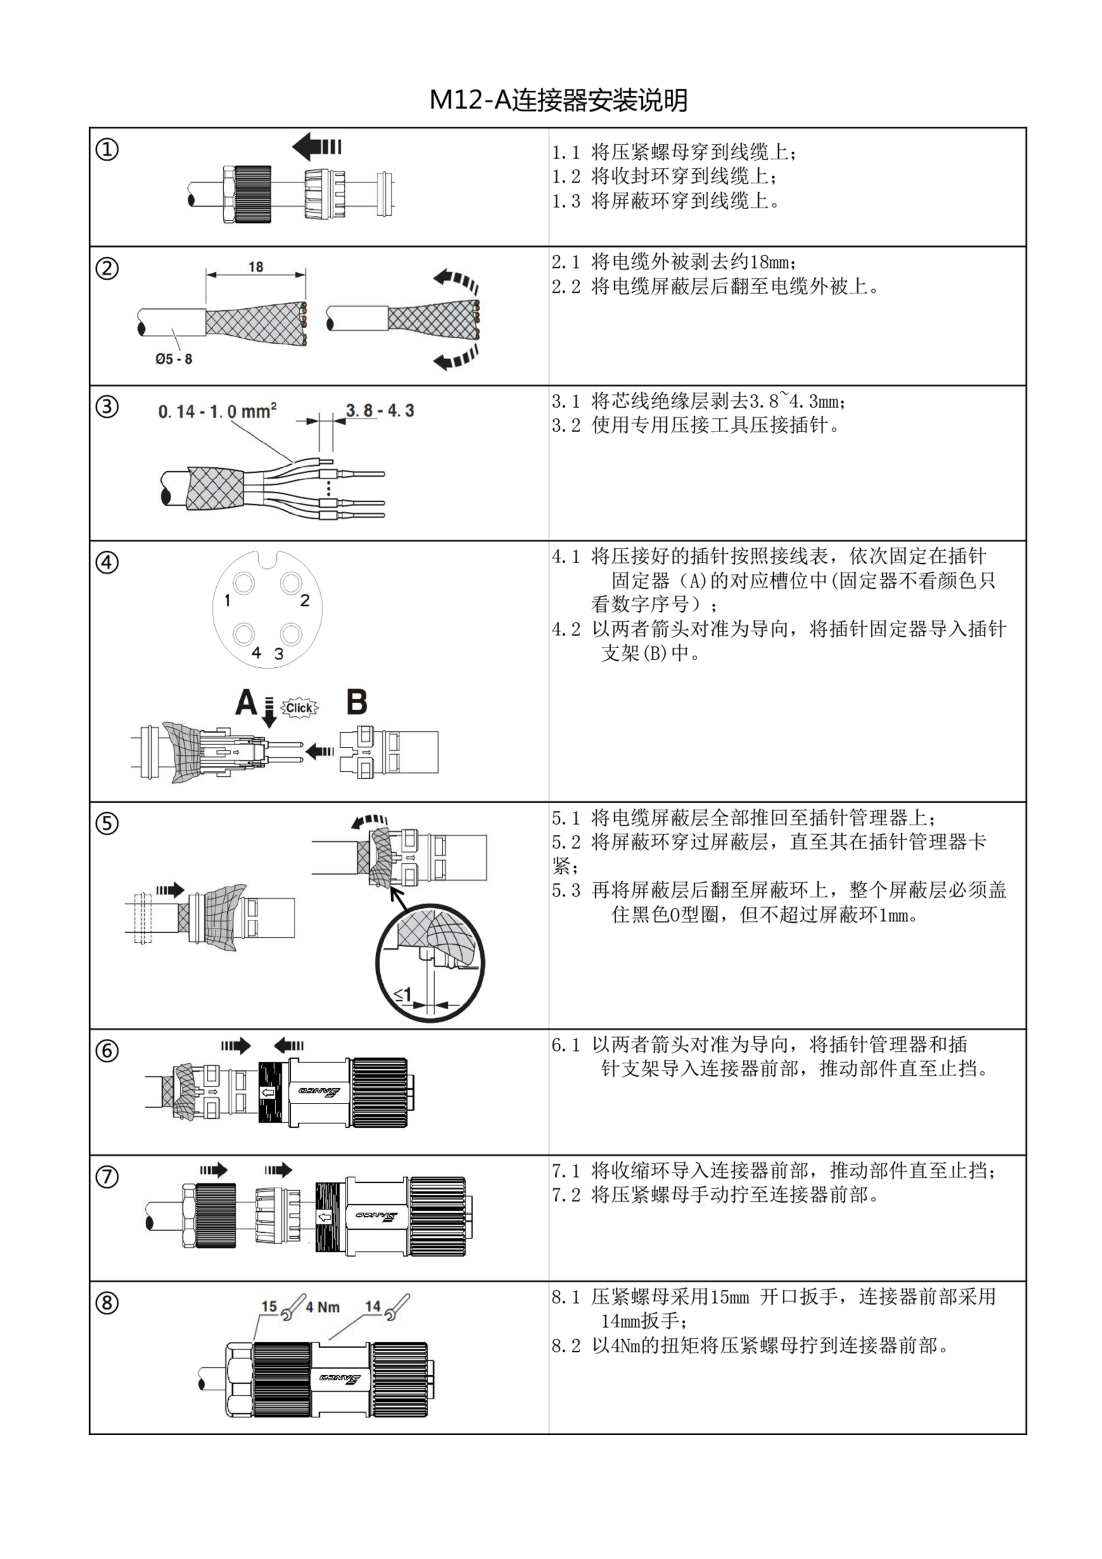
\includegraphics[width=0.8\textwidth]{A-code connection.png}
        \caption{A-code plug connection}
    \end{figure}
    \item Lay the Power cable from the power socket to the Power module, after the cable is laid, wiring the cable with the plug according to the pins definition above.
    \begin{table}
        \centering
        \caption{A-code Plug pin definition}
        \begin{tabular}{|p{2cm}|p{3cm}|p{2cm}|p{6cm}|}
            \hline
            \toprule
            PIN No. & Function & Core Color \\
            \midrule
            L & L & RED \\ \hline
            N & N & BLACK \\ \hline
            E & PE & WHITE \\ \hline
            \bottomrule
        \end{tabular}
    \end{table}
    \item Select the RGME module and Installation Mounting from the equipment list, and fix them with M6 × 7 cross countersunk head screw. The relative position can be adjusted up and down according to the mutual influence of the actual installation positions on site.\\
    \begin{center}
        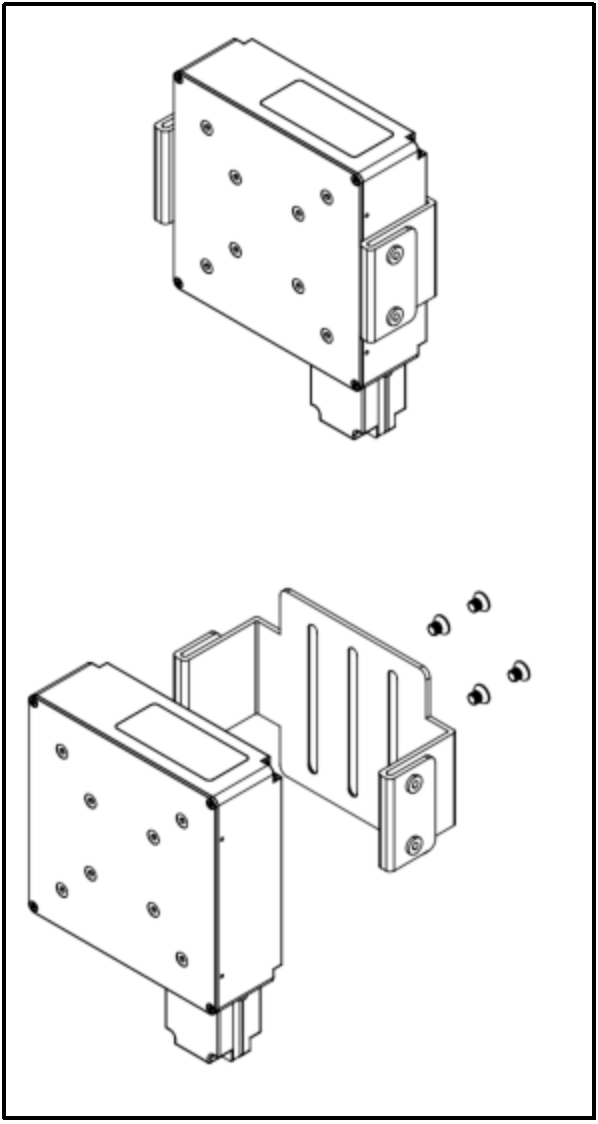
\includegraphics[width=0.2\textwidth]{RGME Mounting.png}
    \end{center}
    \item Select the Power module and Installation Mounting from the equipment list, and fix them with M6 × 7 cross countersunk head screw. The relative position can be adjusted up and down according to the mutual influence of the actual installation positions on site.\\     
    \begin{center}
        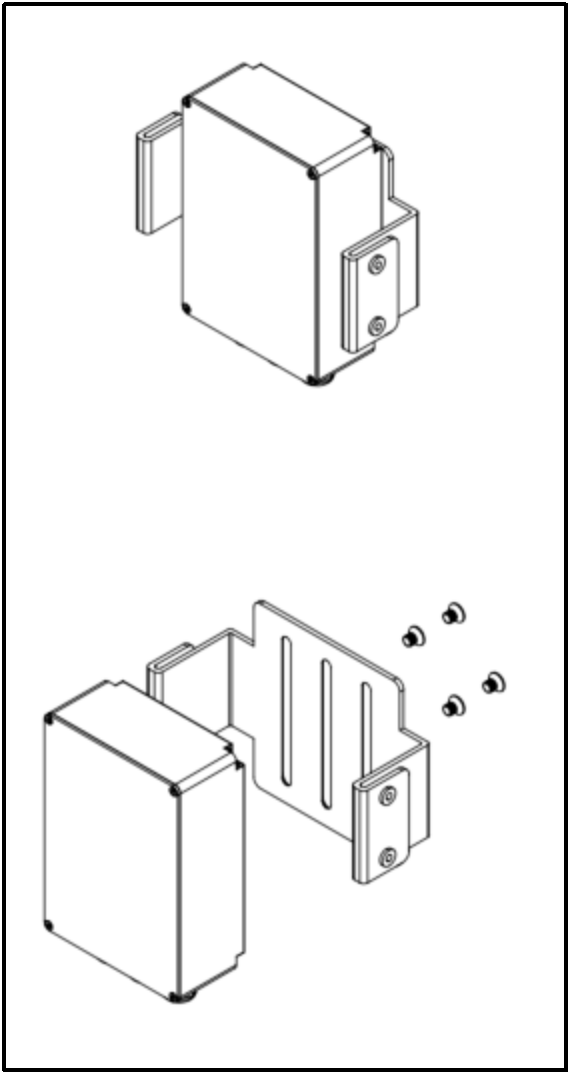
\includegraphics[width=0.2\textwidth]{Battery Mounting.png}
    \end{center}
    \item Tighten the screws with a torque of 10 N·m, and use a marker pen to draw a line as a mark to prevent loosening.\\
    \begin{center}
        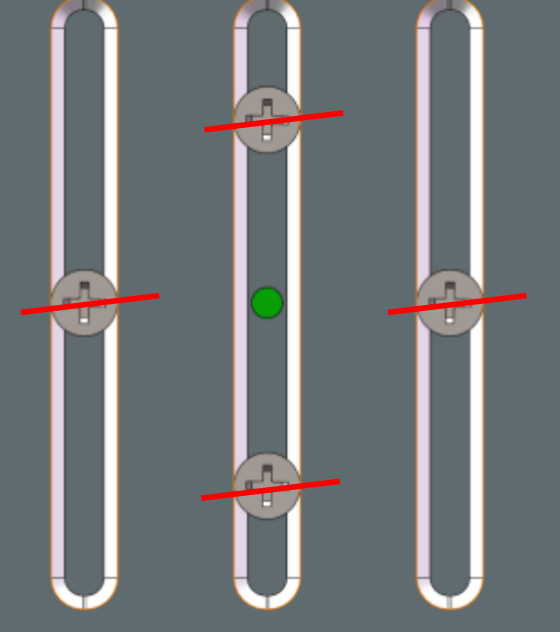
\includegraphics[width=0.3\textwidth]{Mark1.png}
    \end{center}
\end{enumerate}
\subsubsection{Installation on Car}
\begin{enumerate}
    \item Pick up the RGME module with the mounting, put it into the dedicated position inside the structure beam on car behind the decoration panel near door 1.\\
    \begin{center}
        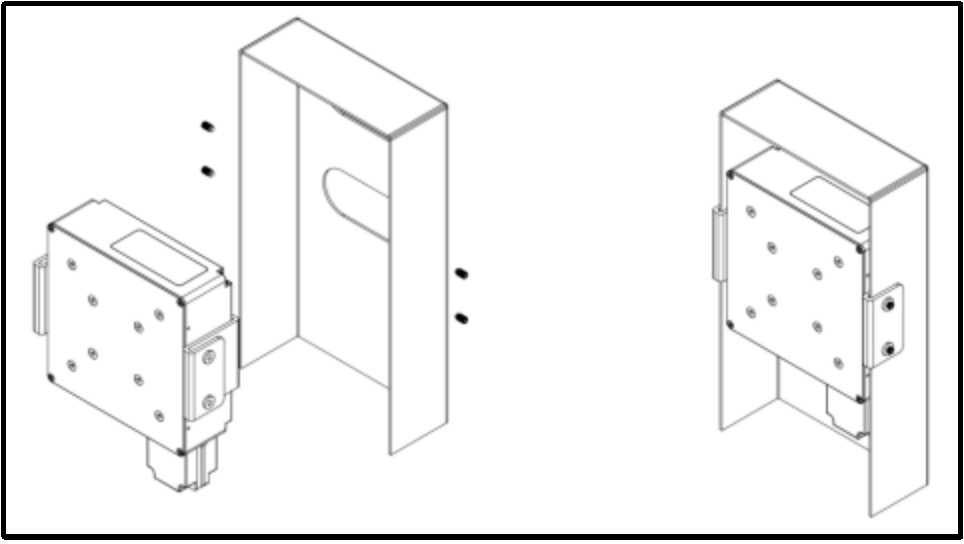
\includegraphics[width=0.5\textwidth]{RGME ready.png}
    \end{center}
    \item Screw it with M5 × 8 304 stainless steel POM nylon tip bolt to the structure beam, and tighten it with a torque of 6.5 N·m.\\
    \item Use a marker pen to draw a line as a mark to prevent loosening.\\
    \begin{center}
        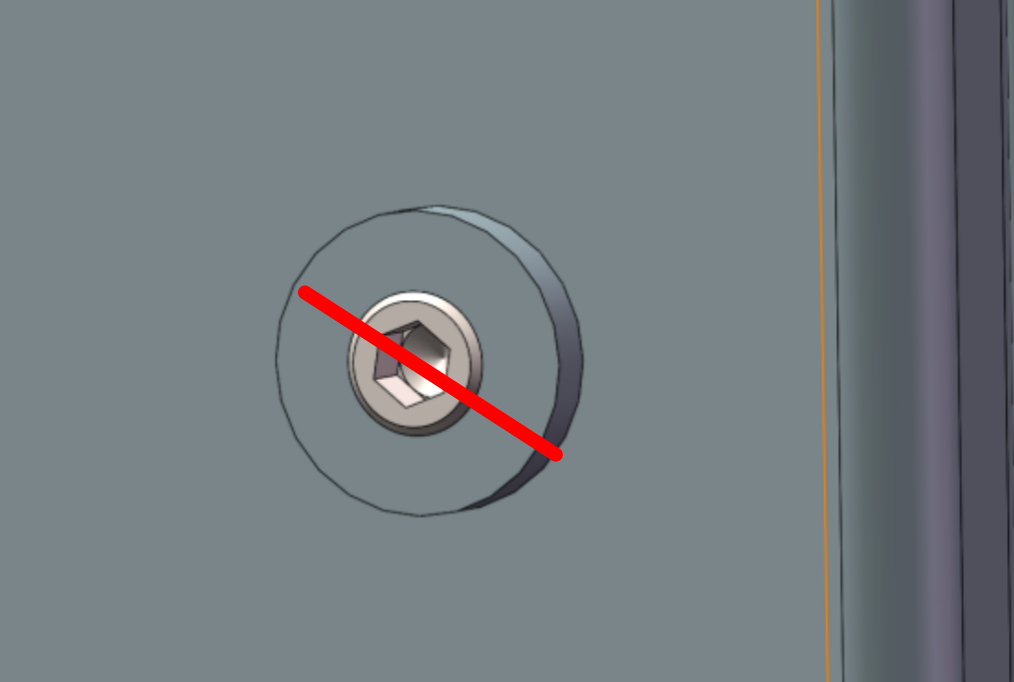
\includegraphics[width=0.5\textwidth]{Mark2.png}
    \end{center}
    \item Pick up the Power module with the mounting, put it into the dedicated position inside the structure beam on car behind the decoration panel near door 1. And also screw it with the same torque and line mark it.\\
    \begin{center}
        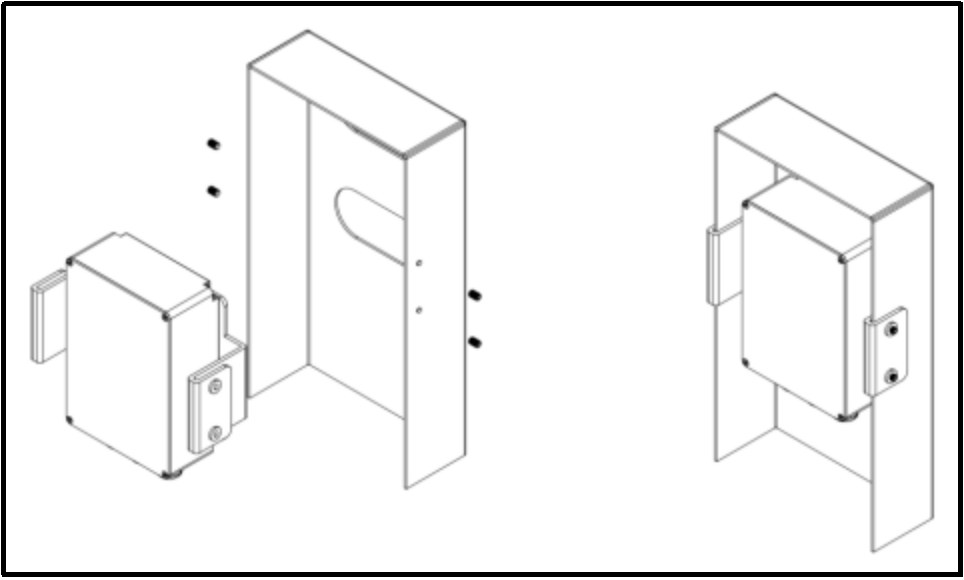
\includegraphics[width=0.5\textwidth]{Battery ready.png}
    \end{center}
    \item Connect the power cable from the Power module to the RGME module 1.\\
    \item Repeat the above steps for the other side of the car's module 2.\\
    \item When tightening all the screws, use Loctite 222 thread locking adhesive to prevent the screws from loosening.\\
\end{enumerate}
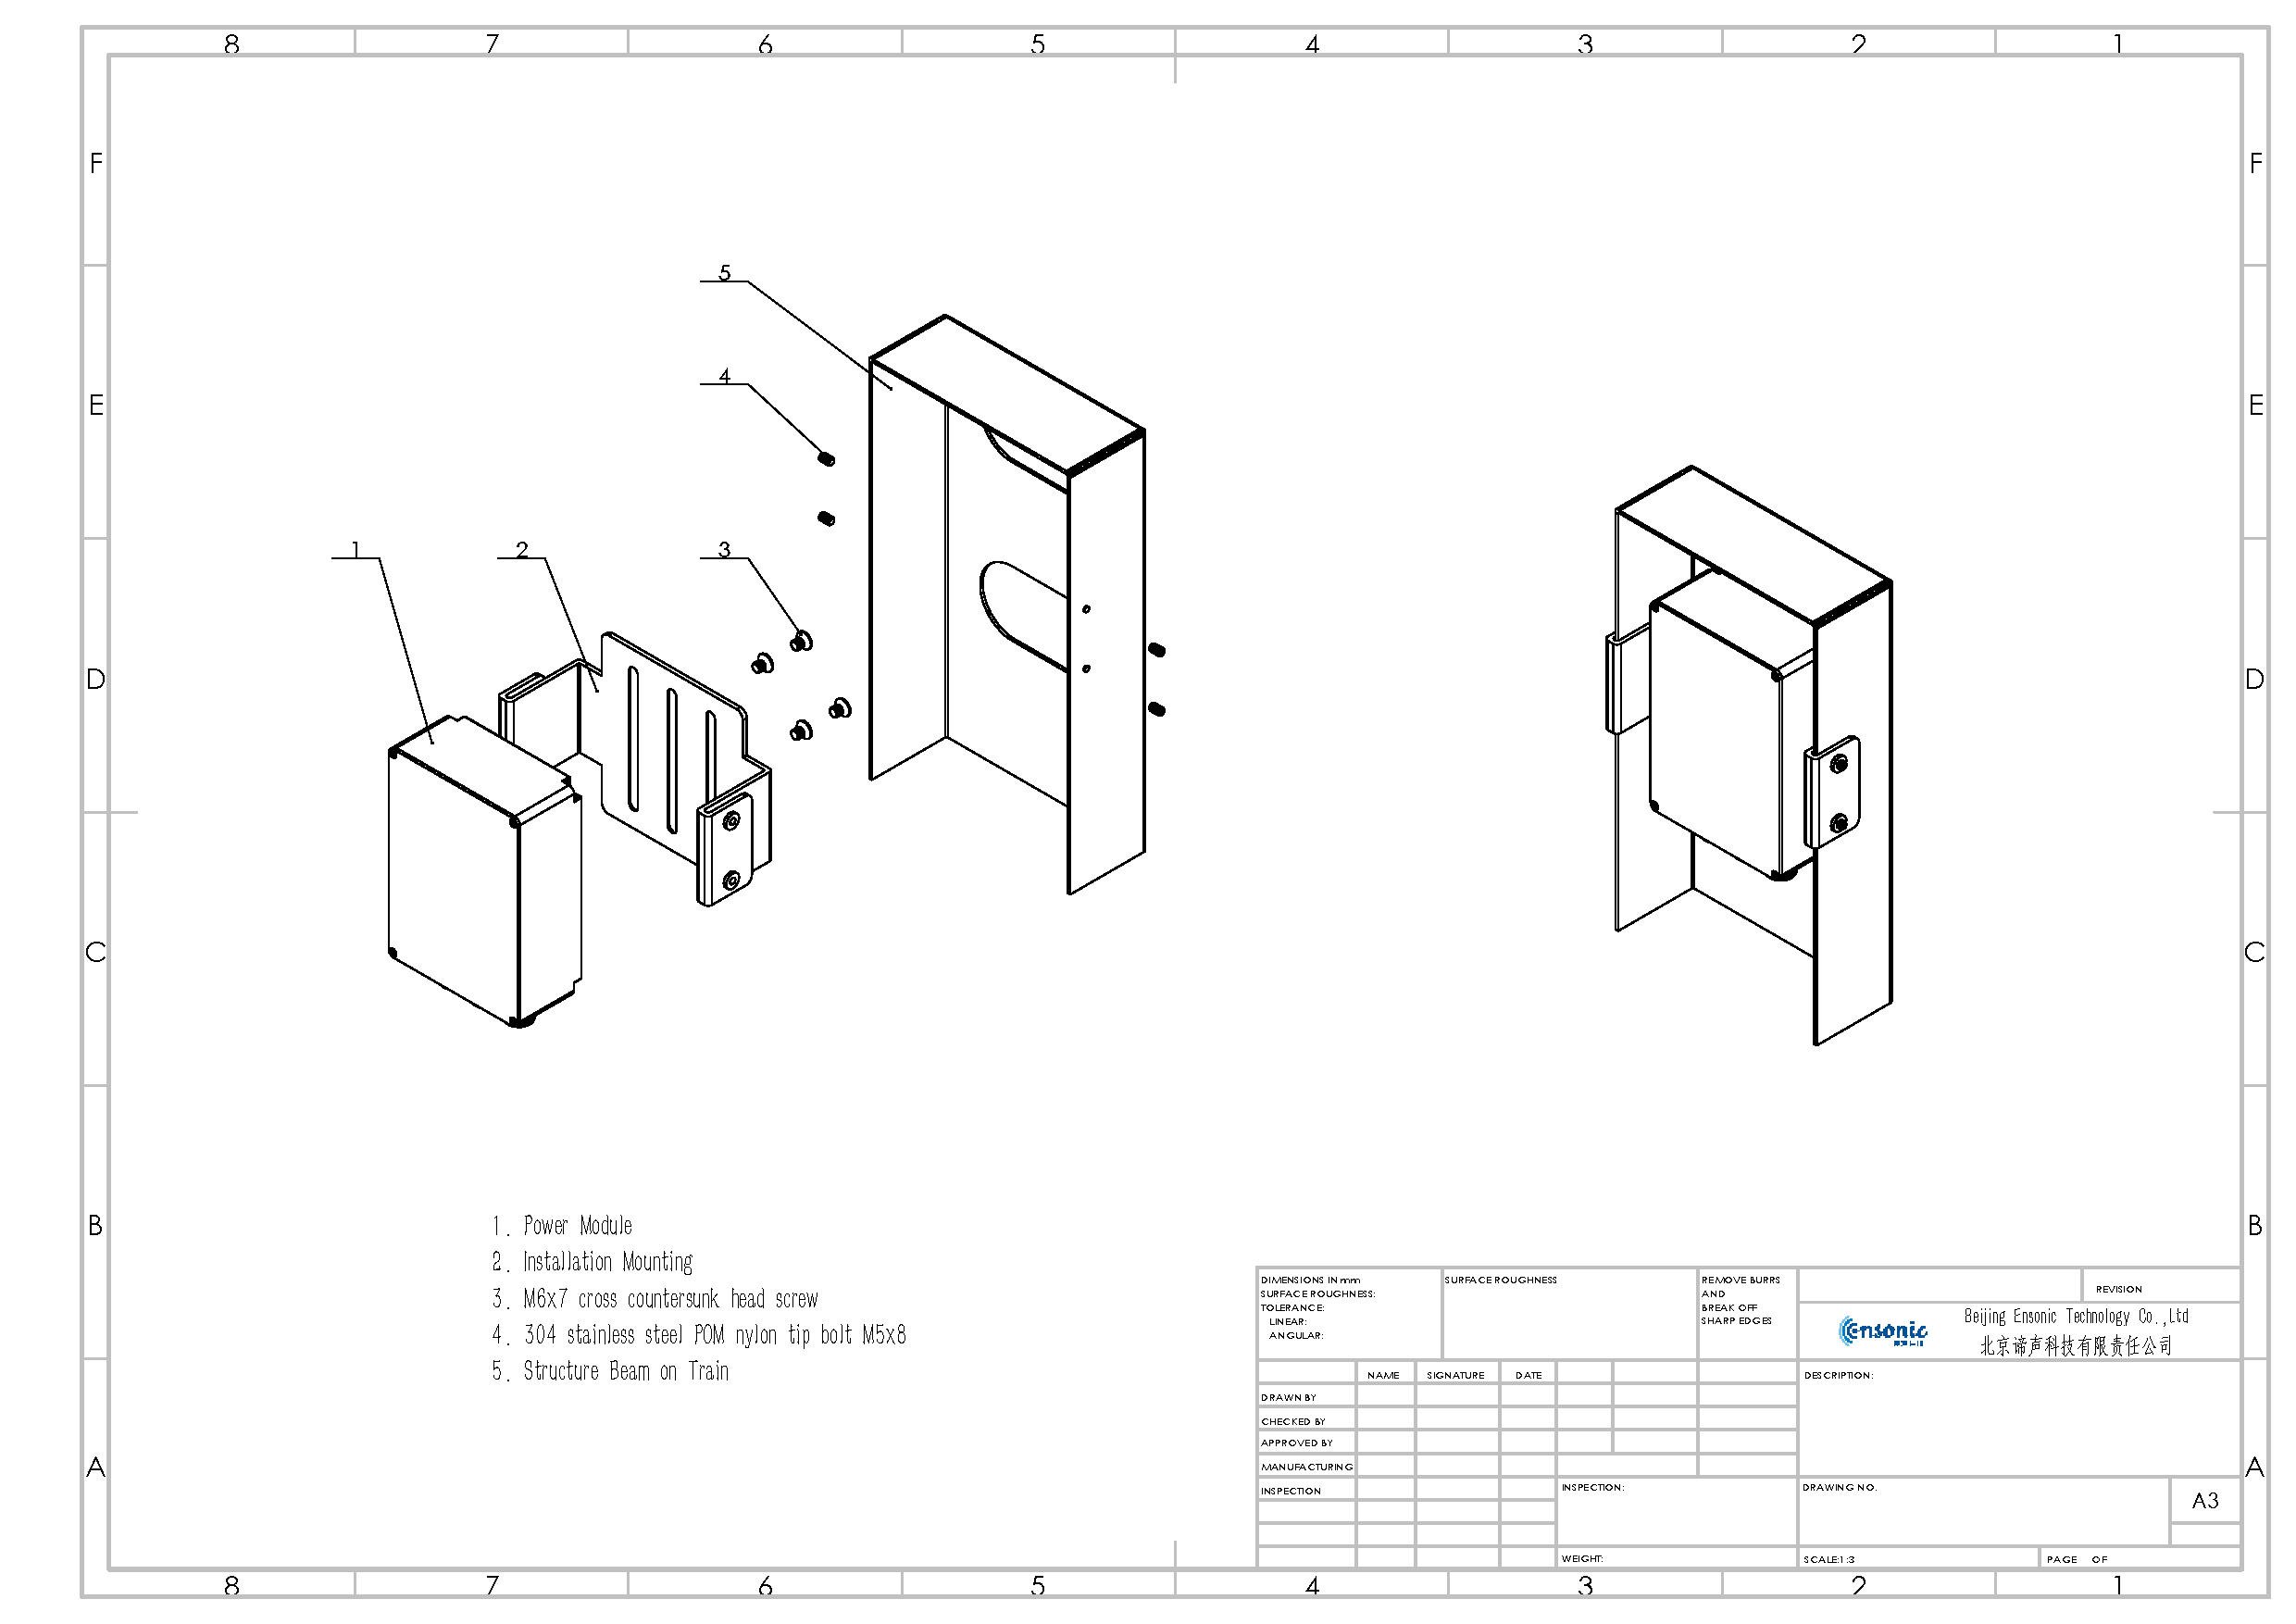
\includepdf[page={1-}, scale=0.75]{./现场安装示意图_电源.pdf}
\subsubsection{Cable Laying and Protection}
\begin{enumerate}
    \begin{figure} [H]
        \centering
        \includegraphics[width=0.8\textwidth]{Cable laying.png}
        \caption{Cable laying diagram}
    \end{figure}
    \item The cable from the power socket to the Power module of A-side is AC220V, and the cable should be laid in a wire groove.
    \item The output cable of the A-side Power module is DC12V, one is connected to the A-side RGME module 1 nearby, and the other is laid to the B-side RGME module through the wire groove.
    \item Label both ends of the cable.
    \item Cables that do not enter the slot should be tied evenly at intervals of 150mm-250mm.
\end{enumerate}
\includepdf[page={1-}, scale=0.75]{./电源安装_布局示意图.pdf}
\subsection{Calculation Report of Installation}

\subsubsection{Each Module with Mounting}

\begin{itemize}
    \item Screw Specifications: Use M6 × 7 cross countersunk screws. M6 means the nominal diameter of the screw is 6mm.
    \item Material characteristics: Scew's material is 304 stainless steel, with a yield strength of 200-300MPa and a median value of 250MPa. Assuming the mounting is made of aluminum alloy, the friction coefficient $\mu$  between the stainless steel screw and the aluminum alloy is about 0.35 (experience value)
    \item Preload calculation: According to the preload formula $F_{max} =\frac {\pi} {4}\times d ^ {2}\times\frac {\sigma_ {s}} {n})$ (the safety factor n is 1.5), substitute the data to get$F_ {max} =\frac {\pi} {4}\times 6 ^ {2}\times\frac {250} {1.5}\approx 11781N$.
    \item Torque calculation: Torque formula$T = K \times F\times d$, the torque coefficient K is related to the surface state of the screw and the lubrication situation. When there is no lubrication, it is usually between 0.18 and 0.22. Take$K = 0.2$ here. Substitute$F_ {max}$ and K and d into,$T = 0.2 \times 11781\times 0.006\approx 14.1N · m$. Considering the convenience and safety of actual installation, it is recommended that the actual torque value be 9 - 11N · m.
\end{itemize}

\subsubsection{Each Module with Structure Beam}

\begin{itemize}
    \item Screw Specifications: Use M5 × 8 304 stainless steel POM nylon tip bolts. M5 means the nominal diameter of the screw is 5mm.
    \item Material Characteristics: 304 stainless steel screws are connected to the steel structure beam, and the friction coefficient is about 0.3 (experience value).
    \item Calculation Idea: The yield strength of 304 stainless steel is generally between 200 - 300MPa, and the safety factor is 1.5. The maximum allowable preload force$F_ {max} =\frac {\pi} {4}\times d ^ {2}\times\frac {\sigma_ {s}} {n}$. For M5 screws,$F_ {max} =\frac {\pi} {4}\times 5 ^ {2}\times\frac {250} {1.5}\approx 6545N$. Torque coefficient K is 0.3.
    \item Torque Calculation: Substitute the torque formula $T = K\times F\times d$,$T = 0.3\times 6545\times 0.005\approx 9.8N · m$. In practical applications, the recommended value is 6-8N · m, which can not only ensure the firmness of the connection, but also prevent damage to screws or structural beams due to excessive torque.
\end{itemize}
\clearpage

\section{Safety Management Plan}
\subsection{Introduction}
This safety management plan is developed to ensure the safe design, installation, operation and maintenance of the RGME device. The plan aims to identify potential hazards, implement appropriate safety measures, and establish procedures for managing safety related issues throughout the project lifecycle.
\subsection{Safety Policy}
The safety of the RGME system is of utmost importance. All activities related to the system, including development, installation, operation, and maintenance, shall comply with relevant safety standards and regulations. The project team is committed to preventing accidents, minimizing risks, ensuring the wellbeing of all personnel involved, and zero tolerance for affecting the safety of the subway system.
\subsection{Harzad Identification and Risk Assessment}
\subsubsection{Harzard Identification}
Identify potential hazards associated with the RGME system, including electrical hazards, mechanical hazards, electromagnetic hazards, and software - related hazards. For example, electrical hazards may include electric shock from exposed wires or malfunctioning power modules, mechanical hazards may involve improper installation leading to component detachment, electromagnetic hazards can be caused by interference with other train systems, and software related hazards may result in unreliable signal accquisition.
\subsubsection{Risk Assessment}
Assess the risks associated with each identified hazard based on the likelihood of occurrence and the potential consequences. Risks are classified as high, medium, or low, and appropriate risk mitigation measures are determined accordingly. For high - risk hazards, immediate actions are taken to reduce the risk to an acceptable level.
\subsection{Safety Measures}
\subsubsubsection{Electrical Safety}
\begin{itemize}
    \item Ensure that all electrical components of the RGME system, such as power modules and wiring, comply with relevant electrical safety standards.
    \item Use appropriate insulation materials and protective enclosures to prevent electric shock.
    \item Implement proper grounding and bonding practices to minimize the risk of electrical faults.
    \item Conduct regular electrical safety inspections during installation and maintenance.
\end{itemize}
\subsubsubsection{Mechanical Safety}
\begin{itemize}
    \item Design the RGME device, power module, and battery module with proper mechanical strength to withstand the vibration and shock of train operation.
    \item Use appropriate mounting brackets and fasteners to ensure the secure installation of components.
    \item Provide clear instructions for installation and maintenance to prevent mechanical failures.
    \item Conduct mechanical integrity checks during installation and periodically during operation.
\end{itemize}
\subsubsubsection{Electromagnetic Safety}
\begin{itemize}
    \item Ensure that the RGME system complies with electromagnetic compatibility standards to prevent interference with other train systems and to ensure its own reliable operation.
    \item Use shielding materials for sensitive components to reduce electromagnetic interference.
    \item Conduct electromagnetic safety inspections during installation and maintenance.
\end{itemize}
\subsubsubsection{Software Safety}
\begin{itemize}
    \item Develop and test the software of the RGME system to ensure its reliability and accuracy in acoustic signal accquisition.
    \item Implement error - handling and recovery mechanisms to prevent software failures from causing safety hazards.
    \item Regularly update the software to address any discovered vulnerabilities.
\end{itemize}
\subsection{Safety Training}
Provide safety training to all personnel involved in the development, installation, operation, and maintenance of the RGME system. The training should cover electrical safety, mechanical safety, electromagnetic safety, and software - related safety issues. Personnel should be trained on how to identify and report safety hazards, as well as how to follow safety procedures.
\subsection{Emergency Response Plan}
Develop an emergency response plan to address safety - related incidents. The plan should include procedures for reporting incidents, evacuating personnel if necessary, and providing first - aid. Emergency response drills should be conducted regularly to ensure that personnel are familiar with the procedures.
\subsection{Monitoring and Review}
Regularly monitor the implementation of safety measures and the effectiveness of the safety management plan. Conduct safety audits and reviews at least quarterly to identify any areas for improvement. Update the safety management plan as needed to address new hazards or changes in the system.
\clearpage
\section{Harzard Log and Risk Register}
\subsection{Operational Harzard Log}
\begin{enumerate}
    \item Inaccurate signal acquisition:
    \begin{itemize}
        \item Harzad Descrption: The RGME device may not accurately capture the acoustic signals from the running gear. Because of the unpredictable environment noise, failure of the RGME device hardware or software.
        \item Potential Consequences: False alarms, misdiagnosis of running gear faults.
        \item Likelihood: Medium.
        \item Risk Level: High.
        \item Mitigation Measures: Regularly check microphone status during system startup; have spare microphones available for quick switched to; establish a maintenance schedule for hardware and software updates.
        \item Responsable Party: Maintenance team.
        \item Monitoring and Review Frequency: Monthly when download data from the USB disk.
    \end{itemize}
    \item Transmission lose:
    \begin{itemize}
        \item Harzad Descrption: The RGME device may lose the 4G transmission due to the electromagnetic interference from the train's electrical systems or other external factors.
        \item Potential Consequences: Loss of NTP time synchronization, data transmission failure.
        \item Likelihood: Medium.
        \item Risk Level: Medium.
        \item Mitigation Measures: ensure the system complies with electromagnetic compatibility standards; establish a maintenance schedule for hardware and software updates.
        \item Responsable Party: Technical team.
        \item Monitoring and Review Frequency: Quarterly.
    \end{itemize}
    \item Power Failure:
    \begin{itemize}
        \item Harzad Descrption: The RGME device may fail to provide power to the system due to power supply failure or power outages.
        \item Potential Consequences: Loss of system functionality, data loss.
        \item Likelihood: Low.(High in the case of Battery mode, cause of battery depletion)
        \item Risk Level: High.
        \item Mitigation Measures: Replace the failed Power module or Battery module; Resetting the RGME device working schedule for every day; establish a maintenance schedule for hardware and software updates to reduce power consumption.
        \item Responsable Party: Technical team.
        \item Monitoring and Review Frequency: Monthly.
    \end{itemize}
    \item Mechanical Failure:
    \begin{itemize}
        \item Harzad Descrption: Incorrect installation of the RGME device, power module, or battery module.
        \item Potential Consequences: Malfunction of the system, inaccurate data collection, potential damage to devices, loosen of the screws even drop off.
        \item Likelihood: Low.
        \item Risk Level: High.
        \item Mitigation Measures: Provide detailed installation training for installers; use torque wrenches and follow strict installation procedures; conduct post installation inspections.
        \item Responsable Party: Installation team.
        \item Monitoring and Review Frequency: Monthly after installation.
    \end{itemize}
    \item Algorithm Glitch:
    \begin{itemize}
        \item Harzad Descrption: Software glitches in the data post-processing or analysis algorithms, due to inappropriate filter settings for the acoustic signal accquisied by installation position.
        \item Potential Consequences: Incorrect fault diagnosis, false alarms, and ineffective predictive maintenance.
        \item Likelihood: Medium.
        \item Risk Level: Medium.
        \item Mitigation Measures: Try different filter settings; conduct regular software updates and maintenance.
        \item Responsable Party: Technical team.
        \item Monitoring and Review Frequency: Monthly when download data from the USB disk.
    \end{itemize}
\end{enumerate}

\subsection{Project Risk Register}
\subsubsection{Management Risks}
\begin{enumerate}
    \item Project Planning:
    \begin{itemize}
        \item Risk Descrption: Inaccurate estimation of project scope, difficulty, and resources.
        \item Potential Consequences: Project delays; cost overruns; failure to meet project goals.
        \item Likelihood: Medium.
        \item Risk Level: High.
        \item Mitigation Measures: Conduct a detailed feasibility study; involve experienced personnel in planning; use project management tools for resource and schedule management.
        \item Responsable Party: Project manager.
        \item Monitoring and Review Frequency: Weekly review of project progress; monthly reassessment of project scope and resources.
    \end{itemize}
    \item Insufficient Resources:
    \begin{itemize}
        \item Risk Descrption: Insufficient human resources, including skilled developers and managers.
        \item Potential Consequences: Project delays; reduced quality of work; potential project failure.
        \item Likelihood: Medium.
        \item Risk Level: High. 
        \item Mitigation Measures: Recruit and train personnel in advance; cross - train team members; establish a talent pipeline for key roles.
        \item Responsable Party: Human resources department.
        \item Monitoring and Review Frequency: Monthly review of personnel resources.
    \end{itemize}
    \item Project Team Communication Issues:
    \begin{itemize}
        \item Risk Descrption: Lack of collaboration and communication among project team members.
        \item Potential Consequences: Reduced productivity; communication breakdowns; potential project delays.
        \item Likelihood: Low.
        \item Risk Level: Medium.
        \item Mitigation Measures: Establish clear communication protocols; conduct regular team meetings and updates; use project management tools for task tracking.
        \item Responsable Party: Project Manager.
        \item Monitoring and Review Frequency: Weekly team meetings; monthly project updates.
    \end{itemize}
    \item Core team members leave the project:
    \begin{itemize}
        \item Risk Descrption: Core team members leave the project.
        \item Potential Consequences:  Knowledge loss; project delays; potential project failure.
        \item Likelihood: Low.
        \item Risk Level: High.
        \item Mitigation Measures: Have succession plans in place; provide attractive incentives for key personnel; document knowledge and processes.
        \item Responsable Party: Project Manager.
        \item Monitoring and Review Frequency: Quarterly review of team member satisfaction and retention.
    \end{itemize}
    \item Project Resources or Budget Transfered:
    \begin{itemize}
        \item Risk Descrption: Superior leadership transfers project resources or budget to other projects.
        \item Potential Consequences: Project delays; cost overruns; potential project failure.
        \item Likelihood: Medium.
        \item Risk Level: High.
        \item Mitigation Measures: Establish clear project priorities with senior management; communicate the importance of the project.
        \item Responsable Party: Project Manager.
        \item Monitoring and Review Frequency: Regular communication with senior management; monitor resource allocation.
    \end{itemize}
\end{enumerate}
\subsubsection{Technical Risks}
\begin{enumerate}
    \item Hardware Compatibility Issues:
    \begin{itemize}
        \item Risk Descrption: Hardware compatibility issues with the RGME device and additional components, such as 4G modules.
        \item Potential Consequences: System failures; compatibility issues; potential data unreliable.
        \item Likelihood: Medium.
        \item Risk Level: High.
        \item Mitigation Measures: Conduct thorough compatibility testing; have contingency plans for integration failures.
        \item Responsable Party: Technical team.
        \item Monitoring and Review Frequency: During integration testing and before deployment; continuously monitor for compatibility issues.
    \end{itemize}
    \item Lack experience in rapid develop :
    \begin{itemize}
        \item Risk Descrption: Lack of experience in developing new features as project requirements change.
        \item Potential Consequences: Delays in function development.
        \item Likelihood: Medium.
        \item Risk Level: Low.
        \item Mitigation Measures: Have a flexible development process; involve experienced developers in the project; conduct regular code reviews.
        \item Responsable Party: Technical team.
        \item Monitoring and Review Frequency: Monthly code reviews; weekly development meetings.
    \end{itemize}
    \item High - level of technical challenges in the project:
    \begin{itemize}
        \item Risk Descrption: The current developers cannot solve the High - level technical challenges in the project.
        \item Potential Consequences: Delays in project schedule; increased costs; potential project failure.
        \item Likelihood: Medium.
        \item Risk Level: High.
        \item Mitigation Measures: Conduct a detailed feasibility study; involve experienced personnel in planning; consult with external experts if needed.
        \item Responsable Party: Project manager.
        \item Monitoring and Review Frequency: Weekly review of project progress.
    \end{itemize}
    \item Out of Quality Control:
    \begin{itemize}
        \item Risk Descrption: Lack of effective testing and quality control.
        \item Potential Consequences: System failures; compatibility issues; potential safety risks.
        \item Likelihood: Low.
        \item Risk Level: High.
        \item Mitigation Measures: Establish a comprehensive testing plan; allocate sufficient resources for testing; conduct peer reviews of test results.
        \item Responsable Party: Testing team.
        \item Monitoring and Review Frequency: Continuously during the development process; review test results weekly.
    \end{itemize}
\end{enumerate}
\subsubsection{Business Risks}
\begin{enumerate}
    \item Sub - contractors or suppliers fail to deliver components on time or with the required quality:
    \begin{itemize}
        \item Risk Descrption: Sub - contractors or suppliers fail to deliver components on time or with the required quality.
        \item Potential Consequences: Delays in project schedule, increased costs, and potential impact on system performance.
        \item Likelihood: Medium.
        \item Risk Level: High.
        \item Mitigation Measures: Select reliable sub - contractors and suppliers; establish contracts with clear delivery and quality requirements; Test components upon delivery.
        \item Responsable Party: Procurement team.
        \item Monitoring and Review Frequency: Before delivery.
    \end{itemize}
    \item Sub - contractors or suppliers go out of business:
    \begin{itemize}
        \item Risk Descrption: Sub - contractors or suppliers go out of business.
        \item Potential Consequences: Supply chain disruptions; increased costs for finding new partners; potential project delays.
        \item Likelihood: Low.
        \item Risk Level: High.
        \item Mitigation Measures: Have contingency plans in place; diversify the supply chain; regularly assess the financial stability of sub - contractors and suppliers.
        \item Responsable Party: Procurement team.
        \item Monitoring and Review Frequency: Quarterly assessment of sub - contractors and suppliers.
    \end{itemize}
\end{enumerate}
\clearpage
\section{Qualitiy Management Plan}
\subsection{Introduction}
This Quality Plan is designed to ensure that the Running Gear Monitoring Equipment (RGME) system meets the required quality standards throughout its development, deployment, and operation. It outlines the quality assurance activities, responsibilities, and procedures to be followed to achieve and maintain the quality of the RGME system.
\subsection{Quality assurance organizational structure and responsibilities}
\begin{table}
    \centering
    \caption{Quality assurance organizational structure and responsibilities}
    \label{tab:order-ratio}
    \begin{tabular}{|c|c|}
        \hline
        \toprule
        Department & Responsibility \\
        \midrule
        Procurement & Screen qualified suppliers to ensure raw material compliance and track incoming problems \\ \hline
        Production & Production according to process standards, including tracking and supervising print circuit board, SMT, PCBA, etc. Record production data and control process quality. \\   \hline
        Test & Testing of purchased raw materials; testing of work in progress and finished products according to internal requirements \\   \hline
        Technical & Design product processes, formulate technical specifications, and provide technical support for quality issues \\ \hline
        \bottomrule
    \end{tabular}
\end{table}

\clearpage
\section{MMI Design}

{\bfseries\emph{The following MMI is only for professional operators, please do not operate it without professional training.}}
\subsection{Device Info}

The device info page shows the basic information of the RGME device, including the device status, software version, firmware version, and hardware information. The product SN is a unique identifier for each RGME device.

\begin{figure} [H]
    \centering
    \includegraphics[width=1\textwidth]{MMI_deviceinfo.png}
    \caption{Device Info}
\end{figure}

\subsection{Sampling Configurations}

The sampling configurations page allows the user to set the sampling rate, filters, gain and other parameters related to the data acquisition process. The default sampling rate is 48KHz.
\begin{figure} [H]
    \centering
    \includegraphics[width=1\textwidth]{MMI_sampleconfig.png}
    \caption{Sampling Configurations}
\end{figure}

\subsection{Storage Configurations}

The storage configurations page allows the user to set the storage mode, storage path, and other parameters related to the data storage process. The default storage mode is SD card storage. In MTR porject, the data will be stored in the external USB disk.
\begin{figure} [H]
    \centering
    \includegraphics[width=1\textwidth]{MMI_storageconfig.png}
    \caption{Storage Configurations}
\end{figure}

\subsection{Network Configurations}

The network configurations page allows the user to set the network mode, IP address, and other parameters related to the network connection. The default network mode is manual. The default IP address is 192.168.0.xxx, where xxx is the last three digits of the product SN.
\begin{figure} [H]
    \centering
    \includegraphics[width=1\textwidth]{MMI_network.png}
    \caption{Network Configurations}
\end{figure}

\subsection{Server Configurations}

The server configurations page allows the user to set the server IP address, port number, and other parameters related to the data transmission process. In MTR project, the data will not be transmitted to the server, so this page is not used.
\begin{figure} [H]
    \centering
    \includegraphics[width=1\textwidth]{MMI_server.png}
    \caption{Server Configurations}
\end{figure}

\subsection{Data Management}

The data management page allows the user to view the data files stored in the device, delete the data files, and format the storage device. User can download the data files to the local computer or to the server. But in MTR project, the data can more easily be get by just remove the USB disk and replace it with a new one.
\begin{figure} [H]
    \centering
    \includegraphics[width=1\textwidth]{MMI_storage_ex.png}
    \caption{Data Management}
\end{figure}

\subsection{Log Report}

The log report page allows the user to view the log files generated by the device, delete the log files, and format the storage device. The log files are used for debugging and troubleshooting purposes. In MTR project, the log files are not used.
\begin{figure} [H]
    \centering
    \includegraphics[width=1\textwidth]{MMI_log.png}
    \caption{Log Report}    
\end{figure}

\clearpage
\section{Complied Standards}
The RGME device needs to be installed in the car carriage of a subway train. Therefore, this device and its accessories need to meet various requirements for on-board equipment. The following standards are applicable:
\begin{itemize}
    \item GB4943.1-2022/IEC62368-1:2018 \\Audio/video,information and communication technology equipment Safety requirements
    \item GB5226-1-2019/IEC60204-1:2016 \\Safety of machinery - Electrical equipment of machines General requirements
    \item GB/T4208-2017/IEC60529:2013 \\Degrees of protection provided by enclosures (IP code)
    \item GB/T17626-2018/IEC61000:2008 \\Electromagnetic compatibility (EMC)
    \item GB/T2423-2016/IEC60068:2012 \\Environmental testing
    \item GB/T21563-2018/IEC61373:2010 \\Railway applications — Rollingstock equipment — Shock and vibrationtests
    \item EN 50155:2017 \\Railway applications — Rolling stock equipment — electronic equipment
\end{itemize}
\clearpage
\subsection{Already Complied Standards}
\subsubsection{GB/T2423-2016/IEC60068:2012 \textit {Environmental testing}}
\includepdf[page={1-}, scale=0.75]{./GB2423.pdf}
\subsubsection{GB/T17626-2018/IEC61000:2008 \textit {Electromagnetic compatibility (EMC)}}
\includepdf[page={1-}, scale=0.75]{./GB17626.pdf}
\subsubsection{GB/T4208-2017/IEC60529:2013 \textit {Degrees of protection provided by enclosures (IP code)}}
\includepdf[page={1-}, scale=0.75]{./GB4208.pdf}
\subsubsection{GB5226-1-2019/IEC60204-1:2016 \textit {Safety of machinery - Electrical equipment of machines General requirements}\\GB4943.1-2022/IEC62368-1:2018 \\Audio/video,information and communication technology equipment Safety requirements}
\includepdf[page={1-}, scale=0.75]{./GB5226.pdf}
\clearpage
\subsection{To Be Complied Standards}
Test listed below will be complied around end of April 2025.
\subsubsection{EN 50155:2017 \textit {Railway applications — Rolling stock equipment — electronic equipment}}

\subsubsection{GB/T21563-2018/IEC61373:2010 \textit {Railway applications — Rollingstock equipment — Shock and vibration tests}}
\clearpage
\section{Factory Test Report}

{\bfseries\emph{The following test report is not the final version, it is just a sample from another test batch. The final version will be provided after the manufacturing and test are completed.}}
\includepdf[page={1-}, scale=0.75]{./硬件测试报告_总览.pdf}
\includepdf[page={1-}, scale=0.75]{./硬件测试报告_功能测试.pdf}
\includepdf[page={1-}, scale=0.75]{./硬件测试报告_声学测试.pdf}
\includepdf[page={1-}, scale=0.75]{./硬件测试报告_稳定性测试.pdf}
\end{document}
